\documentclass[12pt]{article}
\usepackage[margin=0.85in]{geometry}
\usepackage{booktabs,longtable,array}
\usepackage{xcolor}
\usepackage{hyperref}
\usepackage{pdfpages}
\hypersetup{colorlinks=true,linkcolor=blue,urlcolor=blue}
\emergencystretch=2em

% Suite report typography. Keep a local copy for standalone portability.
% Build with LuaLaTeX and an installed, genuine Times New Roman font family.
\usepackage{fontspec}
\setmainfont{Times New Roman}
\usepackage{ragged2e,titlesec,caption,etoolbox}
\titleformat{\section}{\normalfont\bfseries\fontsize{15}{17}\selectfont\raggedright}{\thesection}{0.6em}{}
\titleformat{\subsection}{\normalfont\bfseries\fontsize{15}{17}\selectfont\raggedright}{\thesubsection}{0.6em}{}
\titleformat{\subsubsection}{\normalfont\bfseries\fontsize{15}{17}\selectfont\raggedright}{\thesubsubsection}{0.6em}{}
\titleformat{\paragraph}[runin]{\normalfont\bfseries\fontsize{15}{17}\selectfont}{\theparagraph}{0.6em}{}
\DeclareCaptionFont{reporttext}{\normalfont\rmfamily\fontsize{12}{14}\selectfont}
\captionsetup{font=reporttext,labelfont=normalfont,textfont=normalfont,justification=justified,singlelinecheck=false}
\makeatletter
\renewcommand{\normalsize}{\@setfontsize\normalsize{12}{14}\abovedisplayskip=8pt plus 2pt minus 4pt\belowdisplayskip=8pt plus 2pt minus 4pt\abovedisplayshortskip=0pt plus 2pt\belowdisplayshortskip=5pt plus 2pt minus 2pt}
% Tables may be compact, but never below 10 pt or scaled down as graphics.
\renewcommand{\small}{\@setfontsize\small{10}{12}}
\renewcommand{\footnotesize}{\@setfontsize\footnotesize{10}{12}}
\renewcommand{\scriptsize}{\@setfontsize\scriptsize{10}{12}}
\renewcommand{\tiny}{\@setfontsize\tiny{10}{12}}
\renewcommand{\maketitle}{\par\begingroup\raggedright\normalfont\bfseries\fontsize{15}{17}\selectfont\@title\par\endgroup\vspace{12pt}}
\makeatother
\setlength{\emergencystretch}{3em}
% Consistent article paragraphs in every standalone case and guide narrative.
\setlength{\parindent}{15pt}
\setlength{\parskip}{0pt plus 1pt}
\linespread{1}
% Body prose in individual reports and aggregate summaries is always 12 pt.
\newcommand{\ReportBodyText}{\normalfont\normalsize\justifying}
\AtBeginDocument{\ReportBodyText}

\begin{document}
\newcommand{\GuideTitle}{ELMFIRE Verification Guide}
\input{generated/verification_cover_metadata.tex}
% Report cover: title only, with no subtitle, author block, or date.
\hypersetup{pageanchor=false}
\begin{titlepage}
  \thispagestyle{empty}
  \raggedleft

  \vspace*{0.09\textheight}
  {\color{blue!65!black}\rule{0.82\textwidth}{1.2pt}\par}
  \vspace{1.25cm}

  {\Huge\bfseries
    \GuideTitle\par}

  \vspace{1.1cm}
  {\large\bfseries Authors\par}
  \vspace{0.3cm}
  {\normalsize
    \renewcommand{\arraystretch}{1.12}
    \begin{tabular}{r}
      Yiren Qin \\
      Nikolaos Kalogeropoulos \\
      Daniel San Martin \\
      Adam Laird \\
      Dwi M. J. Purnomo \\
      Mateo Giorgi \\
      Maria Theodore \\
      Kasra Shamsaei \\
      Majid Bavandpour \\
      Arnaud Trouv\'e \\
      Michael J. Gollner \\
      Chris Lautenberger
    \end{tabular}\par
  }

  \vspace{0.75cm}
  {\large\bfseries Affiliations\par}
  \vspace{0.3cm}
  {\normalsize
    \renewcommand{\arraystretch}{1.18}
    \begin{tabular}{r}
      University of California, Berkeley \\
      Cloudfire Inc. \\
      University of Maryland, College Park \\
    \end{tabular}\par}

  \vfill
  {
    \renewcommand{\arraystretch}{1.35}
    \begin{tabular}{@{}r@{}}
      \textbf{ELMFIRE version:} \AggregateELMFIREVersion \\
      \textbf{Compiled:} \today \\
    \end{tabular}
    \par
  }

  \vspace{0.75cm}
  {\color{blue!65!black}\rule{0.82\textwidth}{1.2pt}\par}
  \vspace*{0.045\textheight}
\end{titlepage}
\hypersetup{pageanchor=true}
\pagenumbering{arabic}


\section*{About This Guide}
\phantomsection
\addcontentsline{toc}{section}{About This Guide}
This guide examines whether ELMFIRE reproduces prescribed physical and numerical
responses under controlled conditions. Each case develops an expected response,
defines quantitative comparisons and acceptance criteria, and interprets the
available simulation results. The opening summary presents the calculated
decisions and the computational information available during report preparation.

\clearpage
\tableofcontents
\clearpage

\section{How to Read This Guide}

Start with the verification summary for the recorded computational environment,
declared parallel allocation, and scientific decision table. The
case identifiers in the summary link to the corresponding case-report entries.
The complete case reports follow in numerical order; each presents its own scientific
context, equations, metrics, citations, acceptance criteria, and limitations.

Interpret PASS and FAIL against each case's stated acceptance criteria. Missing
results, incomplete simulations, or an unavailable model capability are shown
as NOT EVALUABLE. A completed simulation or a complete narrative alone does not
establish agreement with the expected response.

The computational environment recorded during report preparation is not
necessarily the environment used for every simulation. Within each case, read
the formulation and derived expectation before interpreting the measured
response. The scope and limitations distinguish the behavior demonstrated by
the prescribed conditions from behavior that remains unverified.

% Generated by tools/generate_summary_reports.py; do not edit by hand.
\clearpage
\section{Verification summary}
\label{sec:verification-summary}
\ReportBodyText
\subsection{Computational environment recorded during report preparation}
The following information describes the environment available during preparation of this guide. It does not establish the environment used for earlier simulations. An available compiler is not necessarily the compiler used to build the model. ELMFIRE was not executed to obtain these observations; an undeclared model release remains unknown.

\begingroup\small
\begin{longtable}{@{}>{\raggedright\arraybackslash}p{0.27\textwidth}>{\raggedright\arraybackslash}p{0.68\textwidth}@{}}
\toprule
Configuration & Recorded value \\
\midrule
\endfirsthead
\toprule
Configuration & Recorded value \\
\midrule
\endhead
\bottomrule
\endlastfoot
Recorded at (Coordinated Universal Time) & 2026-09-15T18:02:20+00:00 \\
Declared ELMFIRE release & not declared \\
Operating system & macOS-15.7.7-arm64-arm-64bit \\
Processor architecture & arm64 \\
Message Passing Interface (MPI) implementation & not available \\
Available Fortran compiler & GNU Fortran (Homebrew GCC 14.2.0\_1) 14.2.0 \\
Python version & CPython 3.12.9 \\
Scientific analysis libraries & NumPy 1.26.4; \allowbreak{}Matplotlib 3.9.2; \allowbreak{}PyYAML 6.0.1; \allowbreak{}Rasterio 1.5.0; \allowbreak{}GDAL not installed; \allowbreak{}Pandas 2.2.2; \allowbreak{}GeoPandas not installed; \allowbreak{}Shapely not installed \\
\end{longtable}
\endgroup\ReportBodyText

\subsection{Comparison type and declared parallel allocation}
The comparison type distinguishes isolated and coupled processes or the spatial scale of validation. The process count is the allocation declared for each case, not a measurement of resources used in an earlier simulation. Missing declarations are not inferred.

\begingroup\scriptsize
\begin{longtable}{@{}>{\raggedright\arraybackslash}p{0.22\textwidth}>{\raggedright\arraybackslash}p{0.48\textwidth}>{\raggedright\arraybackslash}p{0.20\textwidth}@{}}
\toprule
Case & Comparison type & MPI processes \\
\midrule
\endfirsthead
\toprule
Case & Comparison type & MPI processes \\
\midrule
\endhead
\midrule
\multicolumn{3}{r}{Continued on next page} \\
\endfoot
\bottomrule
\endlastfoot
\hyperref[case-detail:case01-bet]{CASE01\_BET} & Coupled-process verification & not declared \\
\hyperref[case-detail:case02-fgr]{CASE02\_FGR} & Coupled-process verification & not declared \\
\hyperref[case-detail:case03-etc]{CASE03\_ETC} & Coupled-process verification & not declared \\
\hyperref[case-detail:case04-sti]{CASE04\_STI} & Coupled-process verification & not declared \\
\hyperref[case-detail:case05-tdw]{CASE05\_TDW} & Coupled-process verification & not declared \\
\hyperref[case-detail:case06-f2d]{CASE06\_F2D} & Coupled-process verification & not declared \\
\hyperref[case-detail:case07-ipc]{CASE07\_IPC} & Coupled-process verification & not declared \\
\hyperref[case-detail:case08-fbc]{CASE08\_FBC} & Coupled-process verification & not declared \\
\hyperref[case-detail:case09-mmd]{CASE09\_MMD} & Coupled-process verification & not declared \\
\hyperref[case-detail:case10-wsr]{CASE10\_WSR} & Coupled-process verification & not declared \\
\hyperref[case-detail:case11-wsc]{CASE11\_WSC} & Coupled-process verification & not declared \\
\hyperref[case-detail:case12-trs]{CASE12\_TRS} & Coupled-process verification & not declared \\
\hyperref[case-detail:case13-prm]{CASE13\_PRM} & Coupled-process verification & not declared \\
\hyperref[case-detail:case14-srs]{CASE14\_SRS} & Coupled-process verification & not declared \\
\hyperref[case-detail:case15-cro]{CASE15\_CRO} & Isolated-process verification & not declared \\
\hyperref[case-detail:case16-nsp]{CASE16\_NSP} & Isolated-process verification & not declared \\
\hyperref[case-detail:case17-scv]{CASE17\_SCV} & Isolated-process verification & not declared \\
\hyperref[case-detail:case18-tcv]{CASE18\_TCV} & Isolated-process verification & not declared \\
\hyperref[case-detail:case19-wth]{CASE19\_WTH} & Coupled-process verification & not declared \\
\hyperref[case-detail:case20-pig]{CASE20\_PIG} & Coupled-process verification & not declared \\
\hyperref[case-detail:case21-wde]{CASE21\_WDE} & Coupled-process verification & not declared \\
\hyperref[case-detail:case22-vsl]{CASE22\_VSL} & Coupled-process verification & not declared \\
\hyperref[case-detail:case23-fqd]{CASE23\_FQD} & Coupled-process verification & not declared \\
\hyperref[case-detail:case24-cxi]{CASE24\_CXI} & Coupled-process verification & not declared \\
\hyperref[case-detail:case25-mqd]{CASE25\_MQD} & Coupled-process verification & not declared \\
\hyperref[case-detail:case26-cnf]{CASE26\_CNF} & Coupled-process verification & not declared \\
\hyperref[case-detail:case27-fbt]{CASE27\_FBT} & Coupled-process verification & not declared \\
\hyperref[case-detail:case28-ova]{CASE28\_OVA} & Coupled-process verification & not declared \\
\hyperref[case-detail:case29-sup]{CASE29\_SUP} & Coupled-process verification & not declared \\
\hyperref[case-detail:case30-mit]{CASE30\_MIT} & Coupled-process verification & not declared \\
\hyperref[case-detail:case31-pft]{CASE31\_PFT} & Coupled-process verification & not declared \\
\hyperref[case-detail:case32-rcv]{CASE32\_RCV} & Coupled-process verification & not declared \\
\hyperref[case-detail:case33-sdo]{CASE33\_SDO} & Coupled-process verification & not declared \\
\hyperref[case-detail:case34-fms]{CASE34\_FMS} & Isolated-process verification & not declared \\
\hyperref[case-detail:case35-wss]{CASE35\_WSS} & Isolated-process verification & not declared \\
\hyperref[case-detail:case36-sls]{CASE36\_SLS} & Isolated-process verification & not declared \\
\hyperref[case-detail:case37-dms]{CASE37\_DMS} & Isolated-process verification & not declared \\
\hyperref[case-detail:case38-lms]{CASE38\_LMS} & Isolated-process verification & not declared \\
\hyperref[case-detail:case39-dhc]{CASE39\_DHC} & Isolated-process verification & not declared \\
\hyperref[case-detail:case40-wsd]{CASE40\_WSD} & Coupled-process verification & not declared \\
\hyperref[case-detail:case41-cfp]{CASE41\_CFP} & Isolated-process verification & not declared \\
\hyperref[case-detail:case42-waf]{CASE42\_WAF} & Coupled-process verification & not declared \\
\hyperref[case-detail:case43-wer]{CASE43\_WER} & Coupled-process verification & not declared \\
\hyperref[case-detail:case44-whp]{CASE44\_WHP} & Coupled-process verification & not declared \\
\hyperref[case-detail:case45-hrs]{CASE45\_HRS} & Coupled-process verification & not declared \\
\hyperref[case-detail:case46-wut]{CASE46\_WUT} & Coupled-process verification & not declared \\
\hyperref[case-detail:case47-uwt]{CASE47\_UWT} & Coupled-process verification & not declared \\
\hyperref[case-detail:case48-wgc]{CASE48\_WGC} & Coupled-process verification & not declared \\
\hyperref[case-detail:case49-wtc]{CASE49\_WTC} & Coupled-process verification & not declared \\
\end{longtable}
\endgroup\ReportBodyText

\subsection{Scientific decision summary}
The decisions below follow the established calculated metrics and case-specific acceptance criteria. Completing a simulation or preparing a report does not establish PASS. Missing or insufficient scientific evidence is reported as NOT EVALUABLE.

\textbf{Total cases:} 49\quad
\textbf{PASS:} 30\quad
\textbf{FAIL:} 12\quad
\textbf{CHARACTERIZED:} 0\quad
\textbf{NOT EVALUABLE:} 7

\begingroup\small
\setlength{\LTpre}{0.8em}
\setlength{\LTpost}{0pt}
\begin{longtable}{@{}>{\raggedright\arraybackslash}p{0.15\textwidth}>{\raggedright\arraybackslash}p{0.16\textwidth}>{\raggedright\arraybackslash}p{0.38\textwidth}>{\raggedright\arraybackslash}p{0.22\textwidth}@{}}
\toprule
Case & Category & Title & Decision \\
\midrule
\endfirsthead
\toprule
Case & Category & Title & Decision \\
\midrule
\endhead
\midrule
\multicolumn{4}{r}{Continued on next page} \\
\endfoot
\bottomrule
\endlastfoot
\hyperref[case-detail:case01-bet]{CASE01\_BET} & Coupled-process verification & \hyperref[case-detail:case01-bet]{Biomass Emission-Time Resolution Independence} & \mbox{\textcolor{green!45!black}{\textbf{PASS}}} \\
\hyperref[case-detail:case02-fgr]{CASE02\_FGR} & Coupled-process verification & \hyperref[case-detail:case02-fgr]{Finite-Duration Firebrand Generation} & \mbox{\textcolor{green!45!black}{\textbf{PASS}}} \\
\hyperref[case-detail:case03-etc]{CASE03\_ETC} & Coupled-process verification & \hyperref[case-detail:case03-etc]{Eulerian Firebrand Transport Convergence} & \mbox{\textcolor{red!75!black}{\textbf{FAIL}}} \\
\hyperref[case-detail:case04-sti]{CASE04\_STI} & Coupled-process verification & \hyperref[case-detail:case04-sti]{Steady Transport and Immediate Ignition} & \mbox{\textcolor{green!45!black}{\textbf{PASS}}} \\
\hyperref[case-detail:case05-tdw]{CASE05\_TDW} & Coupled-process verification & \hyperref[case-detail:case05-tdw]{Firebrand Transport in Time-Dependent Wind} & \mbox{\textcolor{green!45!black}{\textbf{PASS}}} \\
\hyperref[case-detail:case06-f2d]{CASE06\_F2D} & Coupled-process verification & \hyperref[case-detail:case06-f2d]{Two-Dimensional Firebrand-Driven Spread} & \mbox{\textcolor{green!45!black}{\textbf{PASS}}} \\
\hyperref[case-detail:case07-ipc]{CASE07\_IPC} & Coupled-process verification & \hyperref[case-detail:case07-ipc]{Ignition Probability and SFT Convergence} & \mbox{\textcolor{red!75!black}{\textbf{FAIL}}} \\
\hyperref[case-detail:case08-fbc]{CASE08\_FBC} & Coupled-process verification & \hyperref[case-detail:case08-fbc]{Deposited Firebrand Consumption} & \mbox{\textcolor{red!75!black}{\textbf{FAIL}}} \\
\hyperref[case-detail:case09-mmd]{CASE09\_MMD} & Coupled-process verification & \hyperref[case-detail:case09-mmd]{Mixed-Mode Ignition-Delay Effects} & \mbox{\textcolor{green!45!black}{\textbf{PASS}}} \\
\hyperref[case-detail:case10-wsr]{CASE10\_WSR} & Coupled-process verification & \hyperref[case-detail:case10-wsr]{WUI Structural Resolution Sensitivity} & \mbox{\textcolor{orange!75!black}{\textbf{NOT EVALUABLE}}} \\
\hyperref[case-detail:case11-wsc]{CASE11\_WSC} & Coupled-process verification & \hyperref[case-detail:case11-wsc]{WUI Surface-Coupling Synchronization} & \mbox{\textcolor{orange!75!black}{\textbf{NOT EVALUABLE}}} \\
\hyperref[case-detail:case12-trs]{CASE12\_TRS} & Coupled-process verification & \hyperref[case-detail:case12-trs]{WUI Temporal-Resolution Sensitivity} & \mbox{\textcolor{red!75!black}{\textbf{FAIL}}} \\
\hyperref[case-detail:case13-prm]{CASE13\_PRM} & Coupled-process verification & \hyperref[case-detail:case13-prm]{WUI Parametric Response Maps} & \mbox{\textcolor{orange!75!black}{\textbf{NOT EVALUABLE}}} \\
\hyperref[case-detail:case14-srs]{CASE14\_SRS} & Coupled-process verification & \hyperref[case-detail:case14-srs]{Two-Dimensional Spatial-Resolution Sensitivity} & \mbox{\textcolor{orange!75!black}{\textbf{NOT EVALUABLE}}} \\
\hyperref[case-detail:case15-cro]{CASE15\_CRO} & Isolated-process verification & \hyperref[case-detail:case15-cro]{Case 15: Constant rate of spread} & \mbox{\textcolor{green!45!black}{\textbf{PASS}}} \\
\hyperref[case-detail:case16-nsp]{CASE16\_NSP} & Isolated-process verification & \hyperref[case-detail:case16-nsp]{Case 16: No-spread limiting behavior} & \mbox{\textcolor{green!45!black}{\textbf{PASS}}} \\
\hyperref[case-detail:case17-scv]{CASE17\_SCV} & Isolated-process verification & \hyperref[case-detail:case17-scv]{Case 17: Spatial convergence} & \mbox{\textcolor{red!75!black}{\textbf{FAIL}}} \\
\hyperref[case-detail:case18-tcv]{CASE18\_TCV} & Isolated-process verification & \hyperref[case-detail:case18-tcv]{Case 18: Temporal convergence} & \mbox{\textcolor{red!75!black}{\textbf{FAIL}}} \\
\hyperref[case-detail:case19-wth]{CASE19\_WTH} & Coupled-process verification & \hyperref[case-detail:case19-wth]{Case 19: Transient WUI heat flux} & \mbox{\textcolor{green!45!black}{\textbf{PASS}}} \\
\hyperref[case-detail:case20-pig]{CASE20\_PIG} & Coupled-process verification & \hyperref[case-detail:case20-pig]{Case 20: Point ignition and isotropic spread} & \mbox{\textcolor{green!45!black}{\textbf{PASS}}} \\
\hyperref[case-detail:case21-wde]{CASE21\_WDE} & Coupled-process verification & \hyperref[case-detail:case21-wde]{Case 21: Wind-driven elliptical spread} & \mbox{\textcolor{green!45!black}{\textbf{PASS}}} \\
\hyperref[case-detail:case22-vsl]{CASE22\_VSL} & Coupled-process verification & \hyperref[case-detail:case22-vsl]{Case 22: Spread across opposing valley slopes} & \mbox{\textcolor{green!45!black}{\textbf{PASS}}} \\
\hyperref[case-detail:case23-fqd]{CASE23\_FQD} & Coupled-process verification & \hyperref[case-detail:case23-fqd]{Case 23: Spatially varying fuel quadrants} & \mbox{\textcolor{green!45!black}{\textbf{PASS}}} \\
\hyperref[case-detail:case24-cxi]{CASE24\_CXI} & Coupled-process verification & \hyperref[case-detail:case24-cxi]{Case 24: Combined fuel, slope, and wind interactions} & \mbox{\textcolor{green!45!black}{\textbf{PASS}}} \\
\hyperref[case-detail:case25-mqd]{CASE25\_MQD} & Coupled-process verification & \hyperref[case-detail:case25-mqd]{Case 25: Spatially varying moisture quadrants} & \mbox{\textcolor{green!45!black}{\textbf{PASS}}} \\
\hyperref[case-detail:case26-cnf]{CASE26\_CNF} & Coupled-process verification & \hyperref[case-detail:case26-cnf]{Case 26: Surface, passive-crown, and active-crown fire} & \mbox{\textcolor{green!45!black}{\textbf{PASS}}} \\
\hyperref[case-detail:case27-fbt]{CASE27\_FBT} & Coupled-process verification & \hyperref[case-detail:case27-fbt]{Case 27: Lagrangian firebrand generation and transport} & \mbox{\textcolor{red!75!black}{\textbf{FAIL}}} \\
\hyperref[case-detail:case28-ova]{CASE28\_OVA} & Coupled-process verification & \hyperref[case-detail:case28-ova]{Case 28: Overnight spread-rate adjustment} & \mbox{\textcolor{green!45!black}{\textbf{PASS}}} \\
\hyperref[case-detail:case29-sup]{CASE29\_SUP} & Coupled-process verification & \hyperref[case-detail:case29-sup]{Case 29: Initial- and extended-attack suppression} & \mbox{\textcolor{red!75!black}{\textbf{FAIL}}} \\
\hyperref[case-detail:case30-mit]{CASE30\_MIT} & Coupled-process verification & \hyperref[case-detail:case30-mit]{Case 30: Multiple-ignition topology} & \mbox{\textcolor{green!45!black}{\textbf{PASS}}} \\
\hyperref[case-detail:case31-pft]{CASE31\_PFT} & Coupled-process verification & \hyperref[case-detail:case31-pft]{Case 31: Planar-front transport} & \mbox{\textcolor{green!45!black}{\textbf{PASS}}} \\
\hyperref[case-detail:case32-rcv]{CASE32\_RCV} & Coupled-process verification & \hyperref[case-detail:case32-rcv]{Case 32: Raster-orientation covariance} & \mbox{\textcolor{green!45!black}{\textbf{PASS}}} \\
\hyperref[case-detail:case33-sdo]{CASE33\_SDO} & Coupled-process verification & \hyperref[case-detail:case33-sdo]{Case 33: Slope-driven directional spread} & \mbox{\textcolor{green!45!black}{\textbf{PASS}}} \\
\hyperref[case-detail:case34-fms]{CASE34\_FMS} & Isolated-process verification & \hyperref[case-detail:case34-fms]{Case 34: Standard fuel-model Rothermel sweep} & \mbox{\textcolor{green!45!black}{\textbf{PASS}}} \\
\hyperref[case-detail:case35-wss]{CASE35\_WSS} & Isolated-process verification & \hyperref[case-detail:case35-wss]{Case 35: Midflame wind-speed Rothermel sweep} & \mbox{\textcolor{green!45!black}{\textbf{PASS}}} \\
\hyperref[case-detail:case36-sls]{CASE36\_SLS} & Isolated-process verification & \hyperref[case-detail:case36-sls]{Case 36: Slope-factor Rothermel sweep} & \mbox{\textcolor{green!45!black}{\textbf{PASS}}} \\
\hyperref[case-detail:case37-dms]{CASE37\_DMS} & Isolated-process verification & \hyperref[case-detail:case37-dms]{Case 37: Dead-fuel moisture and extinction sweep} & \mbox{\textcolor{green!45!black}{\textbf{PASS}}} \\
\hyperref[case-detail:case38-lms]{CASE38\_LMS} & Isolated-process verification & \hyperref[case-detail:case38-lms]{Case 38: Static live-fuel moisture sweep} & \mbox{\textcolor{green!45!black}{\textbf{PASS}}} \\
\hyperref[case-detail:case39-dhc]{CASE39\_DHC} & Isolated-process verification & \hyperref[case-detail:case39-dhc]{Case 39: Dynamic herbaceous curing sweep} & \mbox{\textcolor{green!45!black}{\textbf{PASS}}} \\
\hyperref[case-detail:case40-wsd]{CASE40\_WSD} & Coupled-process verification & \hyperref[case-detail:case40-wsd]{Case 40: Wind-slope vector and direction sweep} & \mbox{\textcolor{green!45!black}{\textbf{PASS}}} \\
\hyperref[case-detail:case41-cfp]{CASE41\_CFP} & Isolated-process verification & \hyperref[case-detail:case41-cfp]{Case 41: Custom fuel-parameter Rothermel sweep} & \mbox{\textcolor{green!45!black}{\textbf{PASS}}} \\
\hyperref[case-detail:case42-waf]{CASE42\_WAF} & Coupled-process verification & \hyperref[case-detail:case42-waf]{Case 42: Wind-adjustment-factor coupling sweep} & \mbox{\textcolor{green!45!black}{\textbf{PASS}}} \\
\hyperref[case-detail:case43-wer]{CASE43\_WER} & Coupled-process verification & \hyperref[case-detail:case43-wer]{Case 43: WU-E ellipse response} & \mbox{\textcolor{orange!75!black}{\textbf{NOT EVALUABLE}}} \\
\hyperref[case-detail:case44-whp]{CASE44\_WHP} & Coupled-process verification & \hyperref[case-detail:case44-whp]{Case 44: WU-E heat-parameter response} & \mbox{\textcolor{orange!75!black}{\textbf{NOT EVALUABLE}}} \\
\hyperref[case-detail:case45-hrs]{CASE45\_HRS} & Coupled-process verification & \hyperref[case-detail:case45-hrs]{Case 45: WU-E heat-to-urban rate-of-spread response} & \mbox{\textcolor{red!75!black}{\textbf{FAIL}}} \\
\hyperref[case-detail:case46-wut]{CASE46\_WUT} & Coupled-process verification & \hyperref[case-detail:case46-wut]{Case 46: Wildland-to-urban WU-E transition and isolated receivers} & \mbox{\textcolor{red!75!black}{\textbf{FAIL}}} \\
\hyperref[case-detail:case47-uwt]{CASE47\_UWT} & Coupled-process verification & \hyperref[case-detail:case47-uwt]{Case 47: Urban-to-wildland WU-E transition and isolated wildland receivers} & \mbox{\textcolor{orange!75!black}{\textbf{NOT EVALUABLE}}} \\
\hyperref[case-detail:case48-wgc]{CASE48\_WGC} & Coupled-process verification & \hyperref[case-detail:case48-wgc]{Case 48: WU-E uniform-community spatial convergence} & \mbox{\textcolor{red!75!black}{\textbf{FAIL}}} \\
\hyperref[case-detail:case49-wtc]{CASE49\_WTC} & Coupled-process verification & \hyperref[case-detail:case49-wtc]{Case 49: WU-E uniform-community temporal convergence} & \mbox{\textcolor{red!75!black}{\textbf{FAIL}}} \\
\end{longtable}
\endgroup\ReportBodyText

\begin{samepage}
\paragraph{Decision vocabulary.}
PASS and FAIL are case-defined scientific decisions. CHARACTERIZED denotes descriptive validation metrics without a justified acceptance threshold. NOT EVALUABLE denotes missing, unrun, incomplete, unsupported, or otherwise non-decisional evidence.
\end{samepage}


% Generated by tools/generate_summary_reports.py; do not edit by hand.
\clearpage
\IfFileExists{../cases/Verification/coupling_tests/CASE01_BET/report/case_report.pdf}{%
  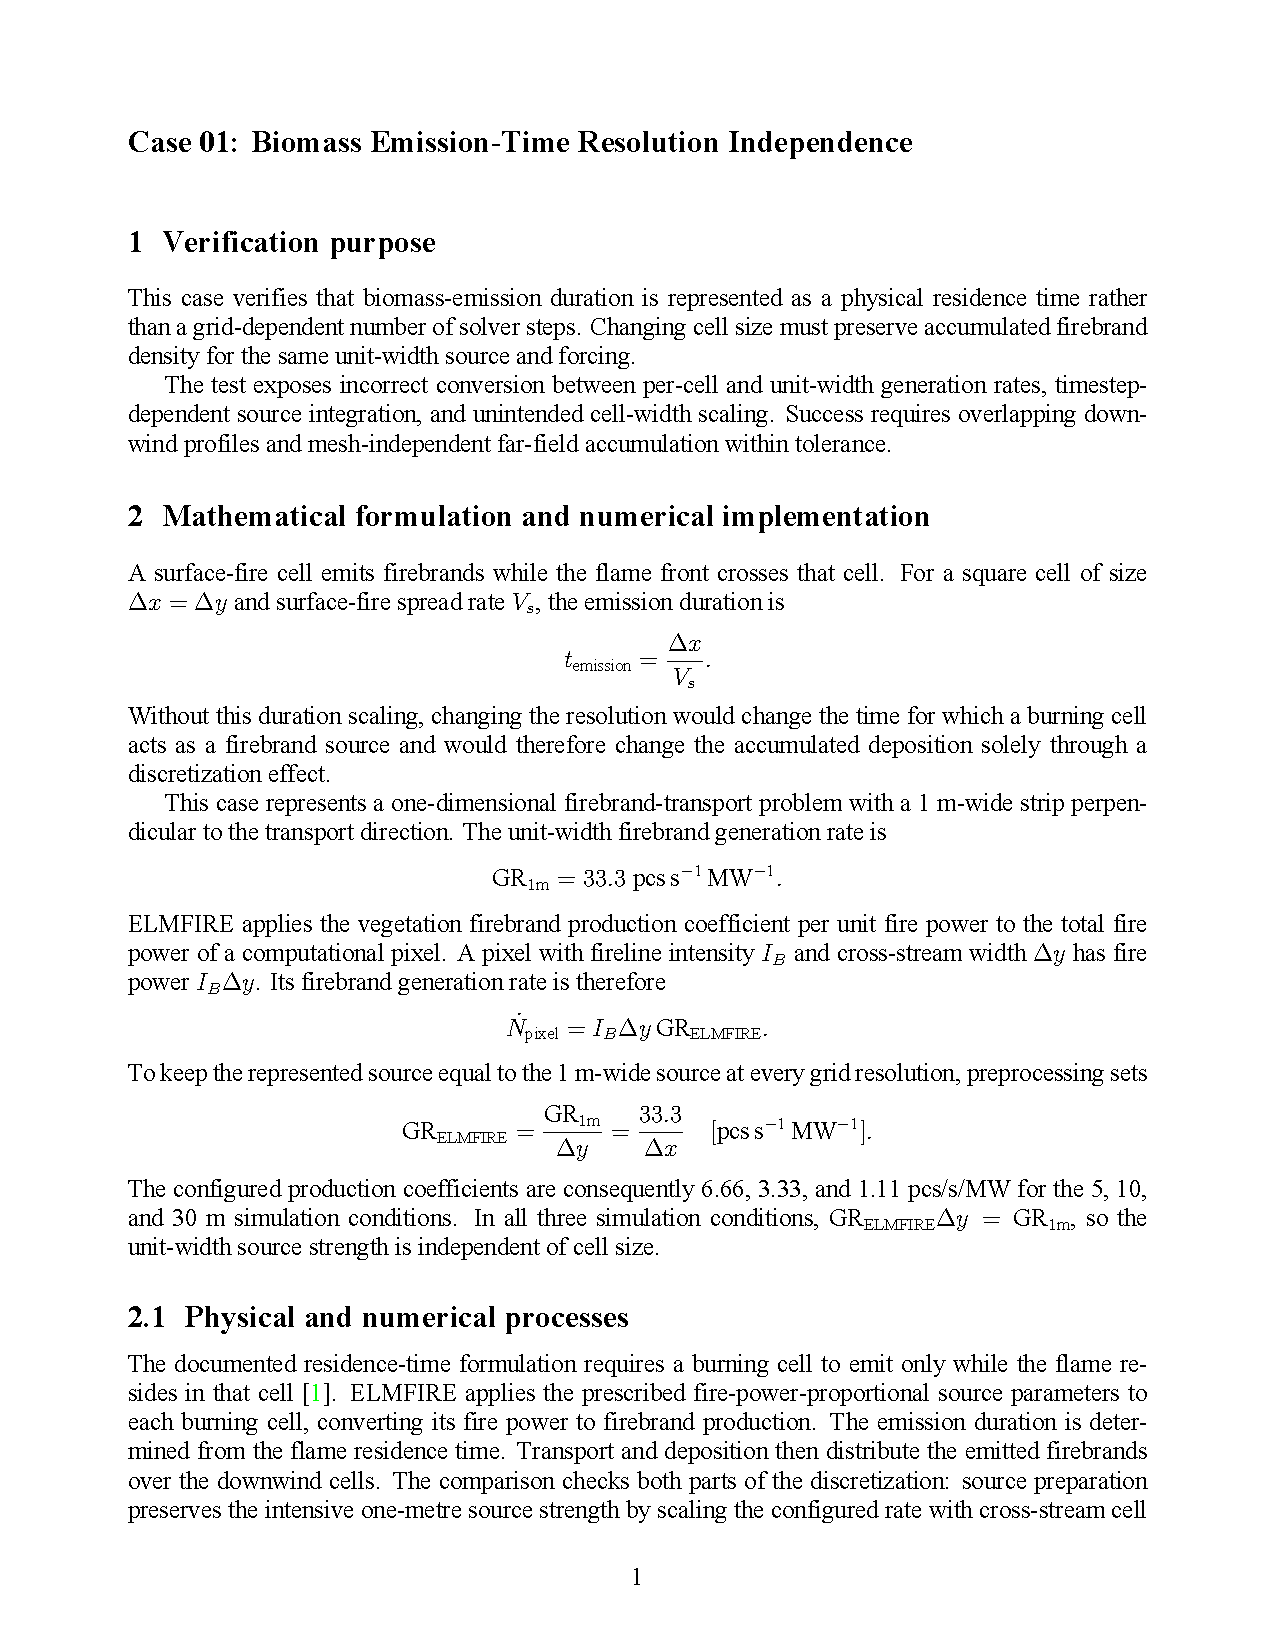
\includepdf[pages=-,pagecommand={\thispagestyle{empty}},addtotoc={1,section,1,{CASE01\_BET -- Biomass Emission-Time Resolution Independence},case-detail:case01-bet}]{../cases/Verification/coupling_tests/CASE01_BET/report/case_report.pdf}%
}{%
  \phantomsection
  \label{case-detail:case01-bet}
  \addcontentsline{toc}{section}{CASE01\_BET -- Biomass Emission-Time Resolution Independence}
  \section*{CASE01\_BET -- Biomass Emission-Time Resolution Independence}
  \textbf{NOT EVALUABLE:} the detailed case description is unavailable.
}

\clearpage
\IfFileExists{../cases/Verification/coupling_tests/CASE02_FGR/report/case_report.pdf}{%
  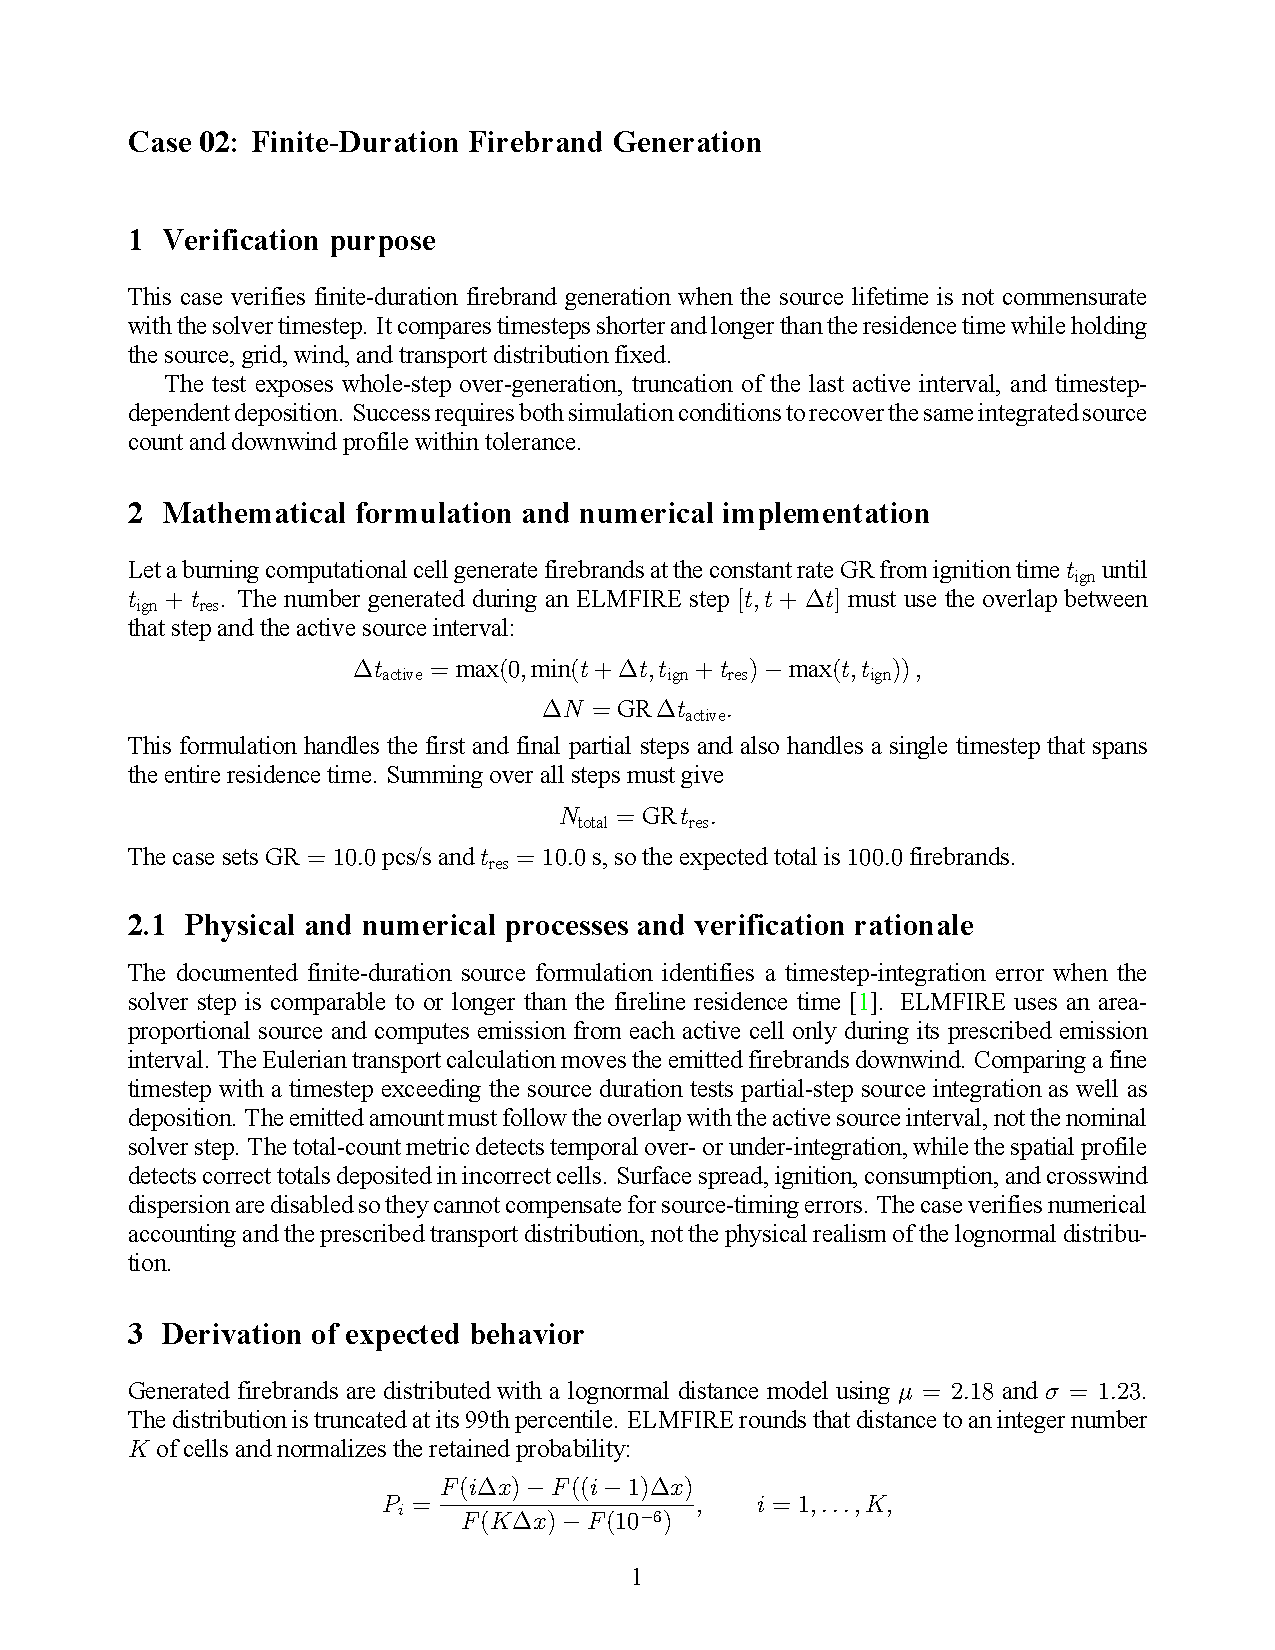
\includepdf[pages=-,pagecommand={\thispagestyle{empty}},addtotoc={1,section,1,{CASE02\_FGR -- Finite-Duration Firebrand Generation},case-detail:case02-fgr}]{../cases/Verification/coupling_tests/CASE02_FGR/report/case_report.pdf}%
}{%
  \phantomsection
  \label{case-detail:case02-fgr}
  \addcontentsline{toc}{section}{CASE02\_FGR -- Finite-Duration Firebrand Generation}
  \section*{CASE02\_FGR -- Finite-Duration Firebrand Generation}
  \textbf{NOT EVALUABLE:} the detailed case description is unavailable.
}

\clearpage
\IfFileExists{../cases/Verification/coupling_tests/CASE03_ETC/report/case_report.pdf}{%
  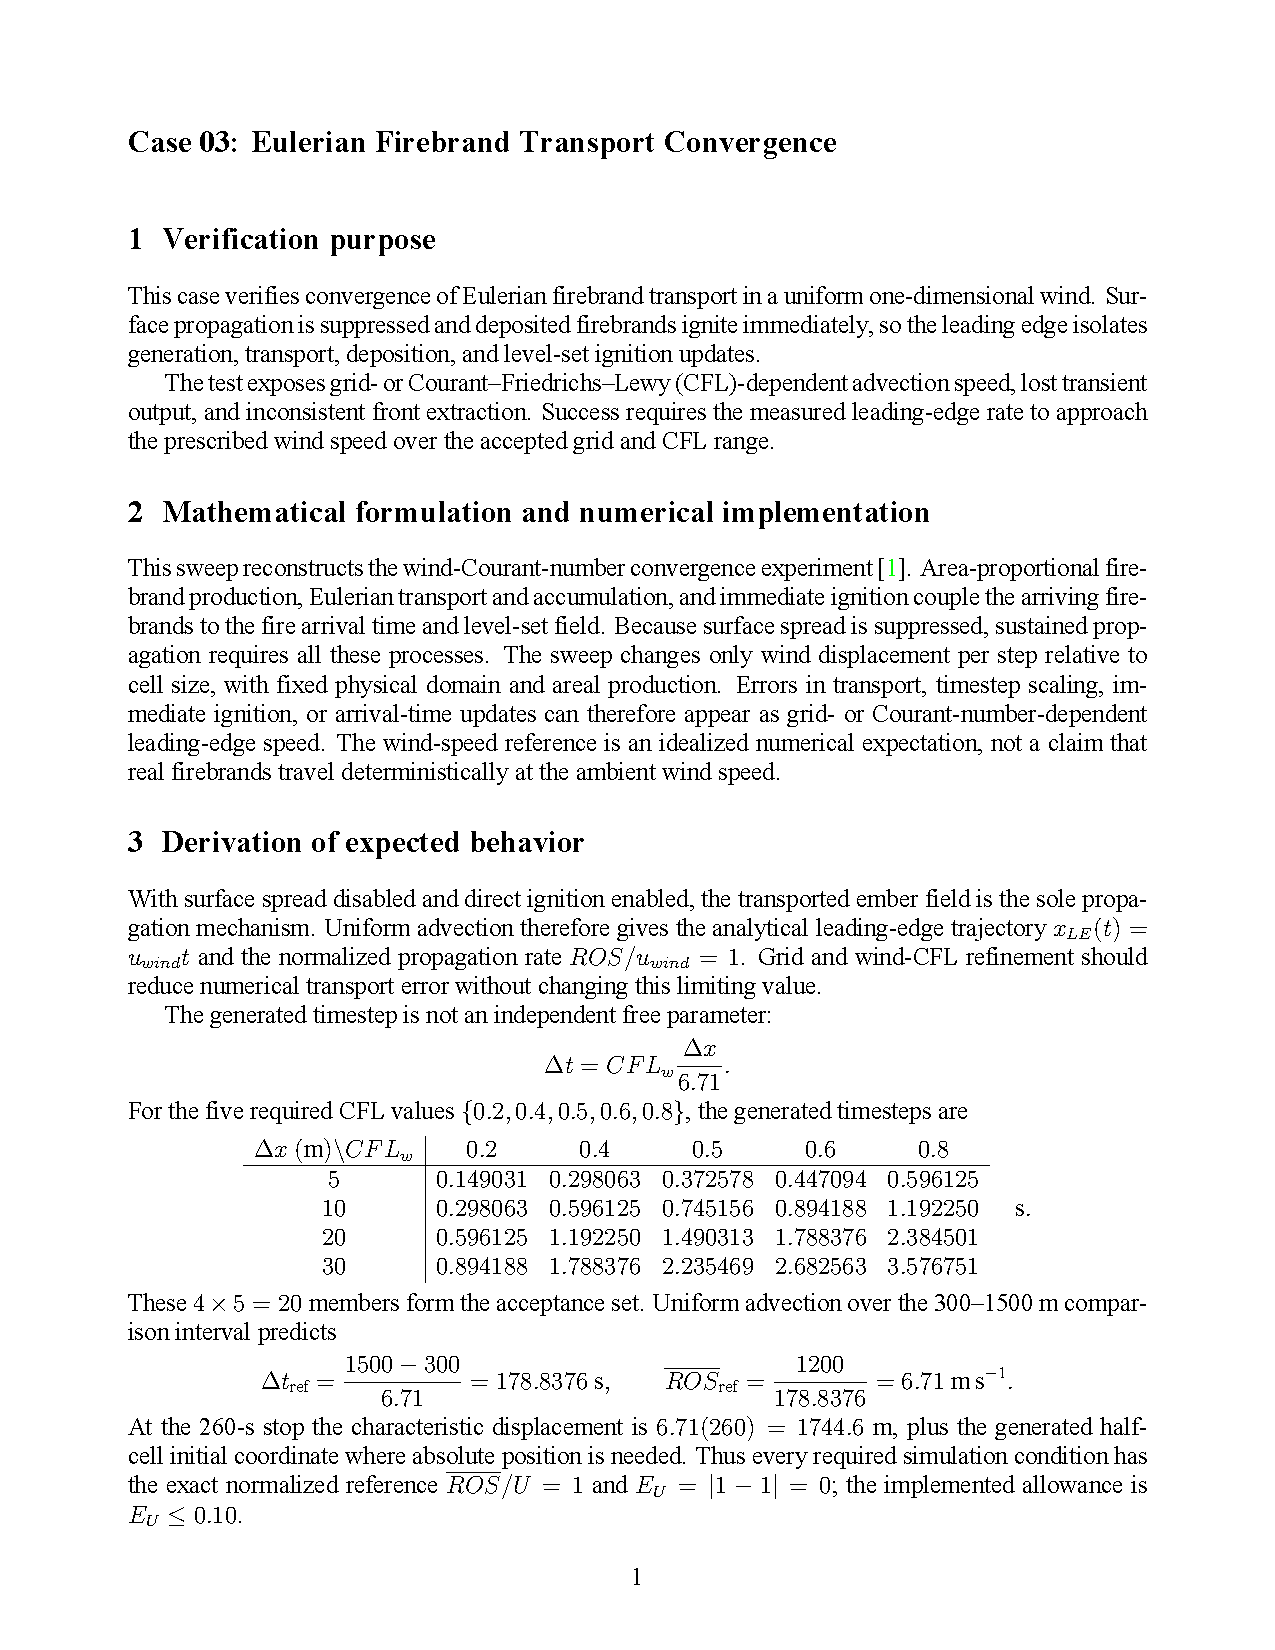
\includepdf[pages=-,pagecommand={\thispagestyle{empty}},addtotoc={1,section,1,{CASE03\_ETC -- Eulerian Firebrand Transport Convergence},case-detail:case03-etc}]{../cases/Verification/coupling_tests/CASE03_ETC/report/case_report.pdf}%
}{%
  \phantomsection
  \label{case-detail:case03-etc}
  \addcontentsline{toc}{section}{CASE03\_ETC -- Eulerian Firebrand Transport Convergence}
  \section*{CASE03\_ETC -- Eulerian Firebrand Transport Convergence}
  \textbf{NOT EVALUABLE:} the detailed case description is unavailable.
}

\clearpage
\IfFileExists{../cases/Verification/coupling_tests/CASE04_STI/report/case_report.pdf}{%
  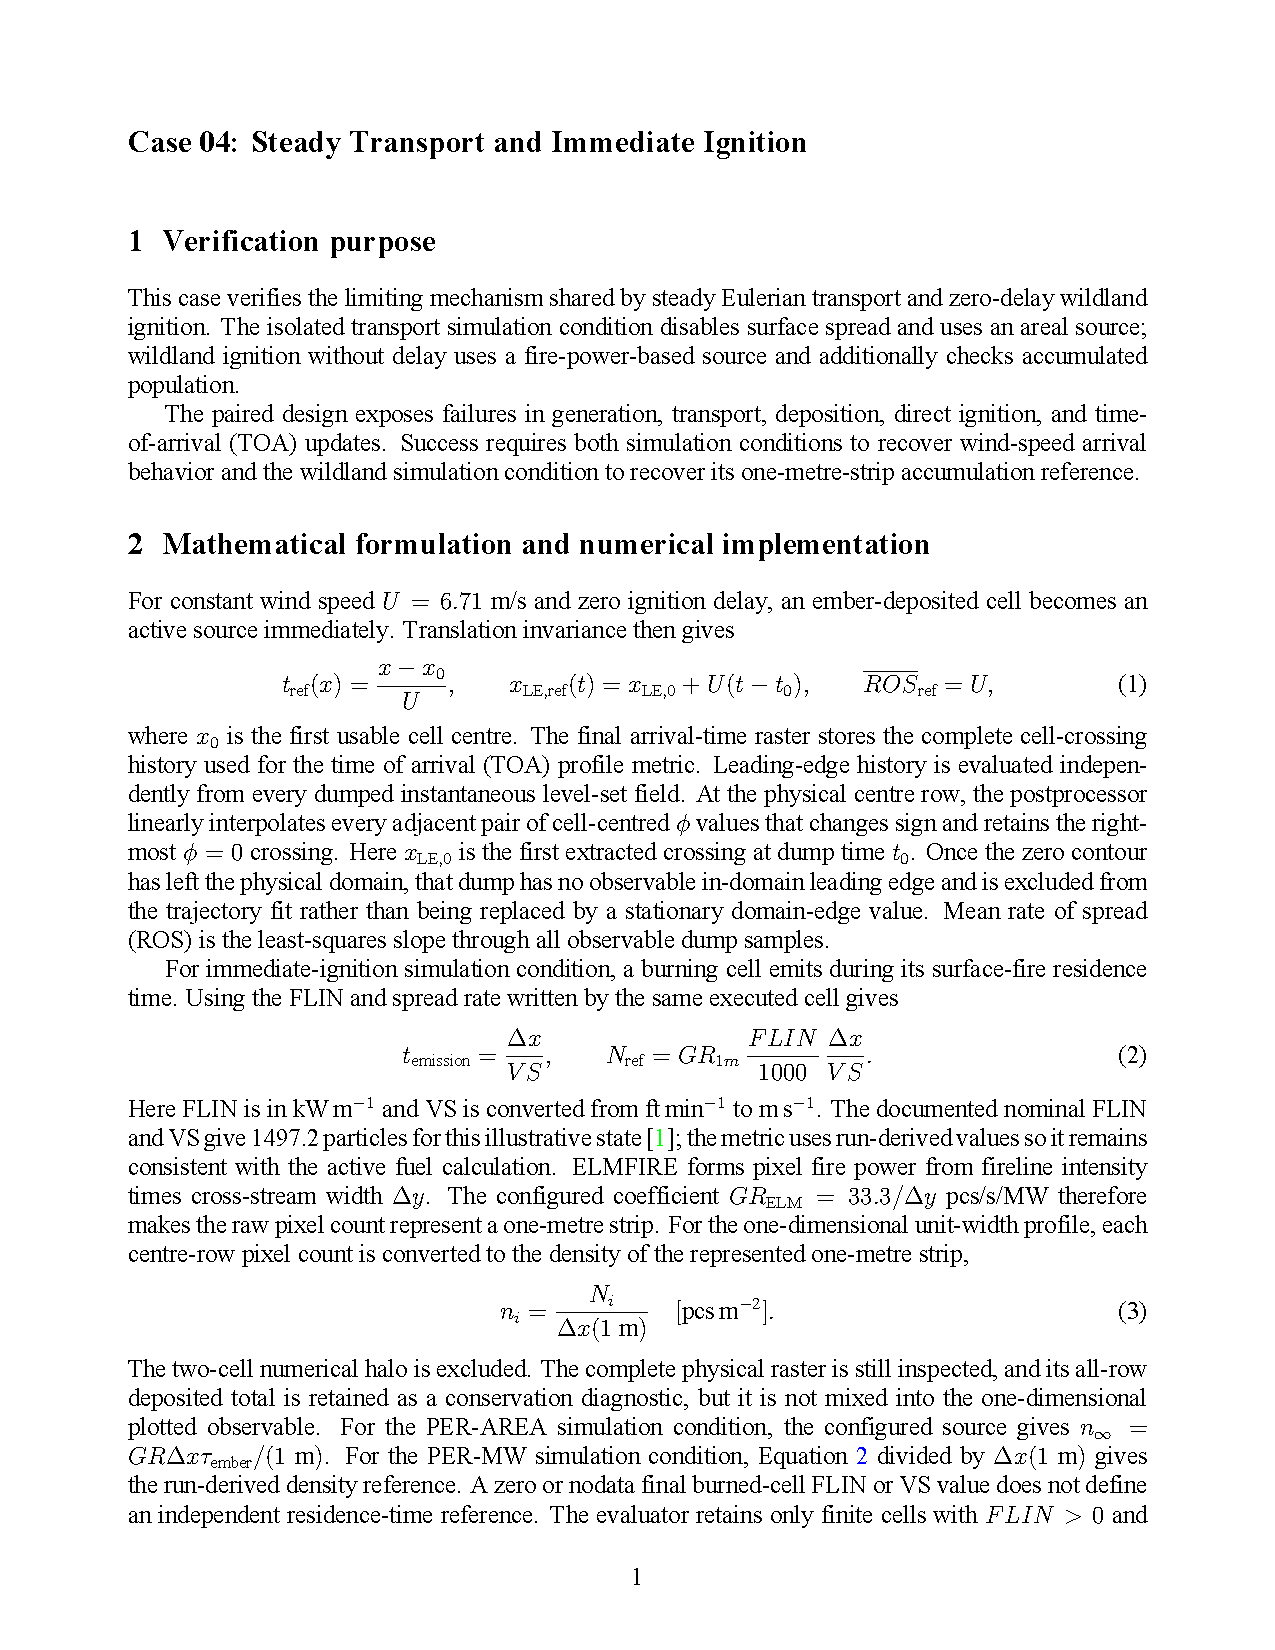
\includepdf[pages=-,pagecommand={\thispagestyle{empty}},addtotoc={1,section,1,{CASE04\_STI -- Steady Transport and Immediate Ignition},case-detail:case04-sti}]{../cases/Verification/coupling_tests/CASE04_STI/report/case_report.pdf}%
}{%
  \phantomsection
  \label{case-detail:case04-sti}
  \addcontentsline{toc}{section}{CASE04\_STI -- Steady Transport and Immediate Ignition}
  \section*{CASE04\_STI -- Steady Transport and Immediate Ignition}
  \textbf{NOT EVALUABLE:} the detailed case description is unavailable.
}

\clearpage
\IfFileExists{../cases/Verification/coupling_tests/CASE05_TDW/report/case_report.pdf}{%
  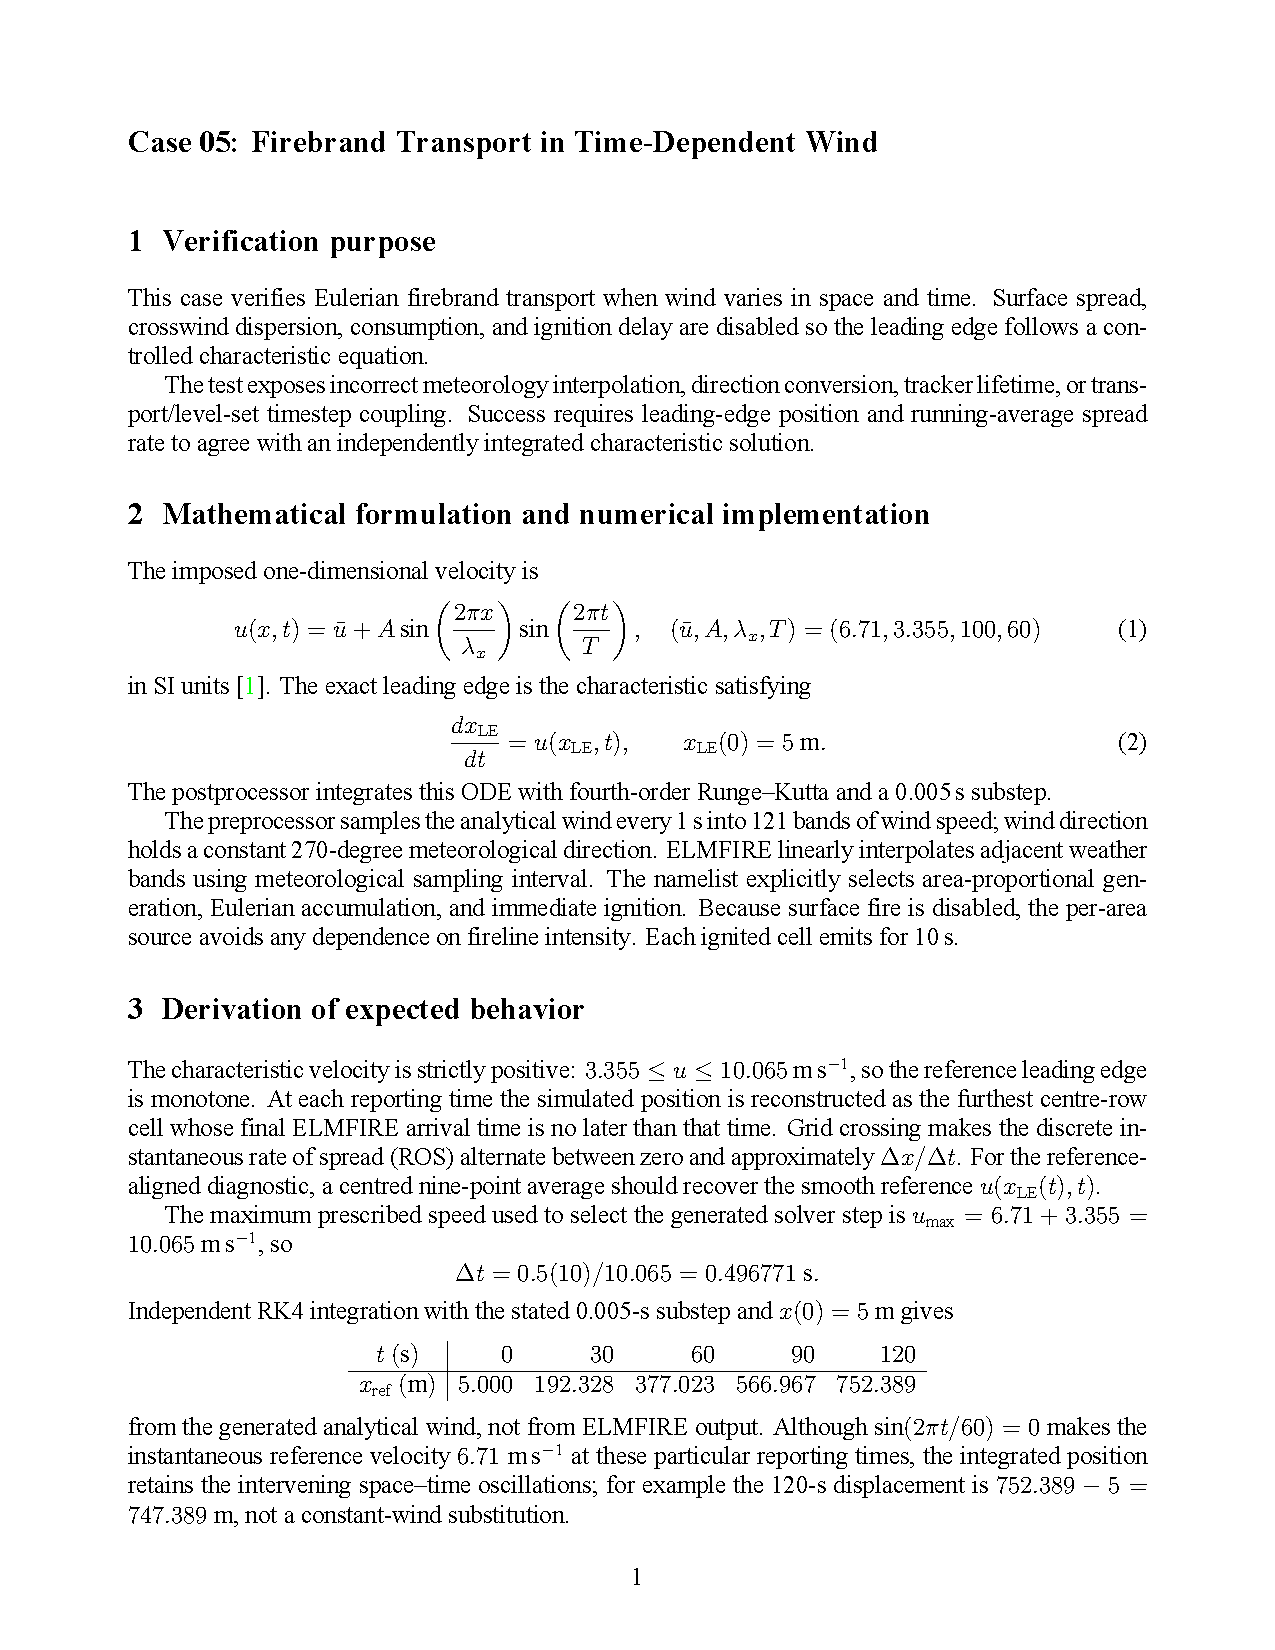
\includepdf[pages=-,pagecommand={\thispagestyle{empty}},addtotoc={1,section,1,{CASE05\_TDW -- Firebrand Transport in Time-Dependent Wind},case-detail:case05-tdw}]{../cases/Verification/coupling_tests/CASE05_TDW/report/case_report.pdf}%
}{%
  \phantomsection
  \label{case-detail:case05-tdw}
  \addcontentsline{toc}{section}{CASE05\_TDW -- Firebrand Transport in Time-Dependent Wind}
  \section*{CASE05\_TDW -- Firebrand Transport in Time-Dependent Wind}
  \textbf{NOT EVALUABLE:} the detailed case description is unavailable.
}

\clearpage
\IfFileExists{../cases/Verification/coupling_tests/CASE06_F2D/report/case_report.pdf}{%
  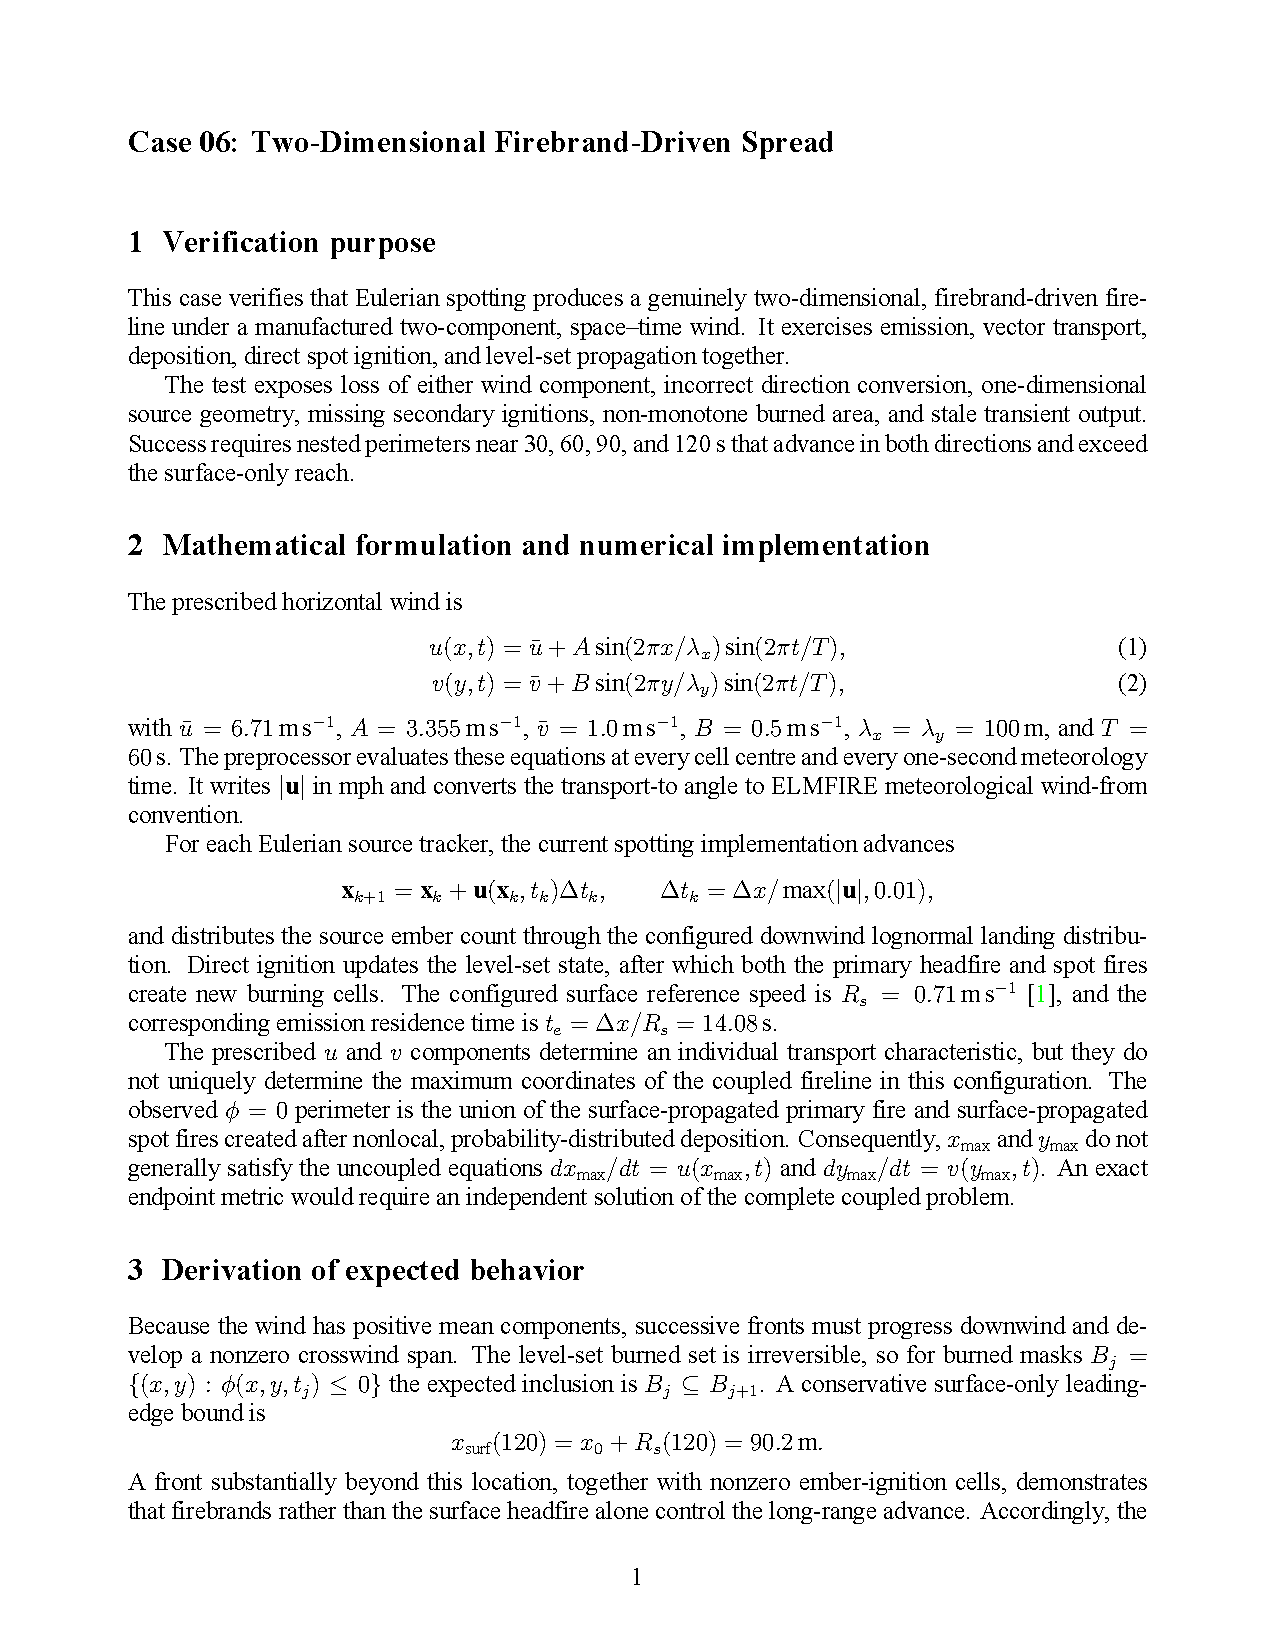
\includepdf[pages=-,pagecommand={\thispagestyle{empty}},addtotoc={1,section,1,{CASE06\_F2D -- Two-Dimensional Firebrand-Driven Spread},case-detail:case06-f2d}]{../cases/Verification/coupling_tests/CASE06_F2D/report/case_report.pdf}%
}{%
  \phantomsection
  \label{case-detail:case06-f2d}
  \addcontentsline{toc}{section}{CASE06\_F2D -- Two-Dimensional Firebrand-Driven Spread}
  \section*{CASE06\_F2D -- Two-Dimensional Firebrand-Driven Spread}
  \textbf{NOT EVALUABLE:} the detailed case description is unavailable.
}

\clearpage
\IfFileExists{../cases/Verification/coupling_tests/CASE07_IPC/report/case_report.pdf}{%
  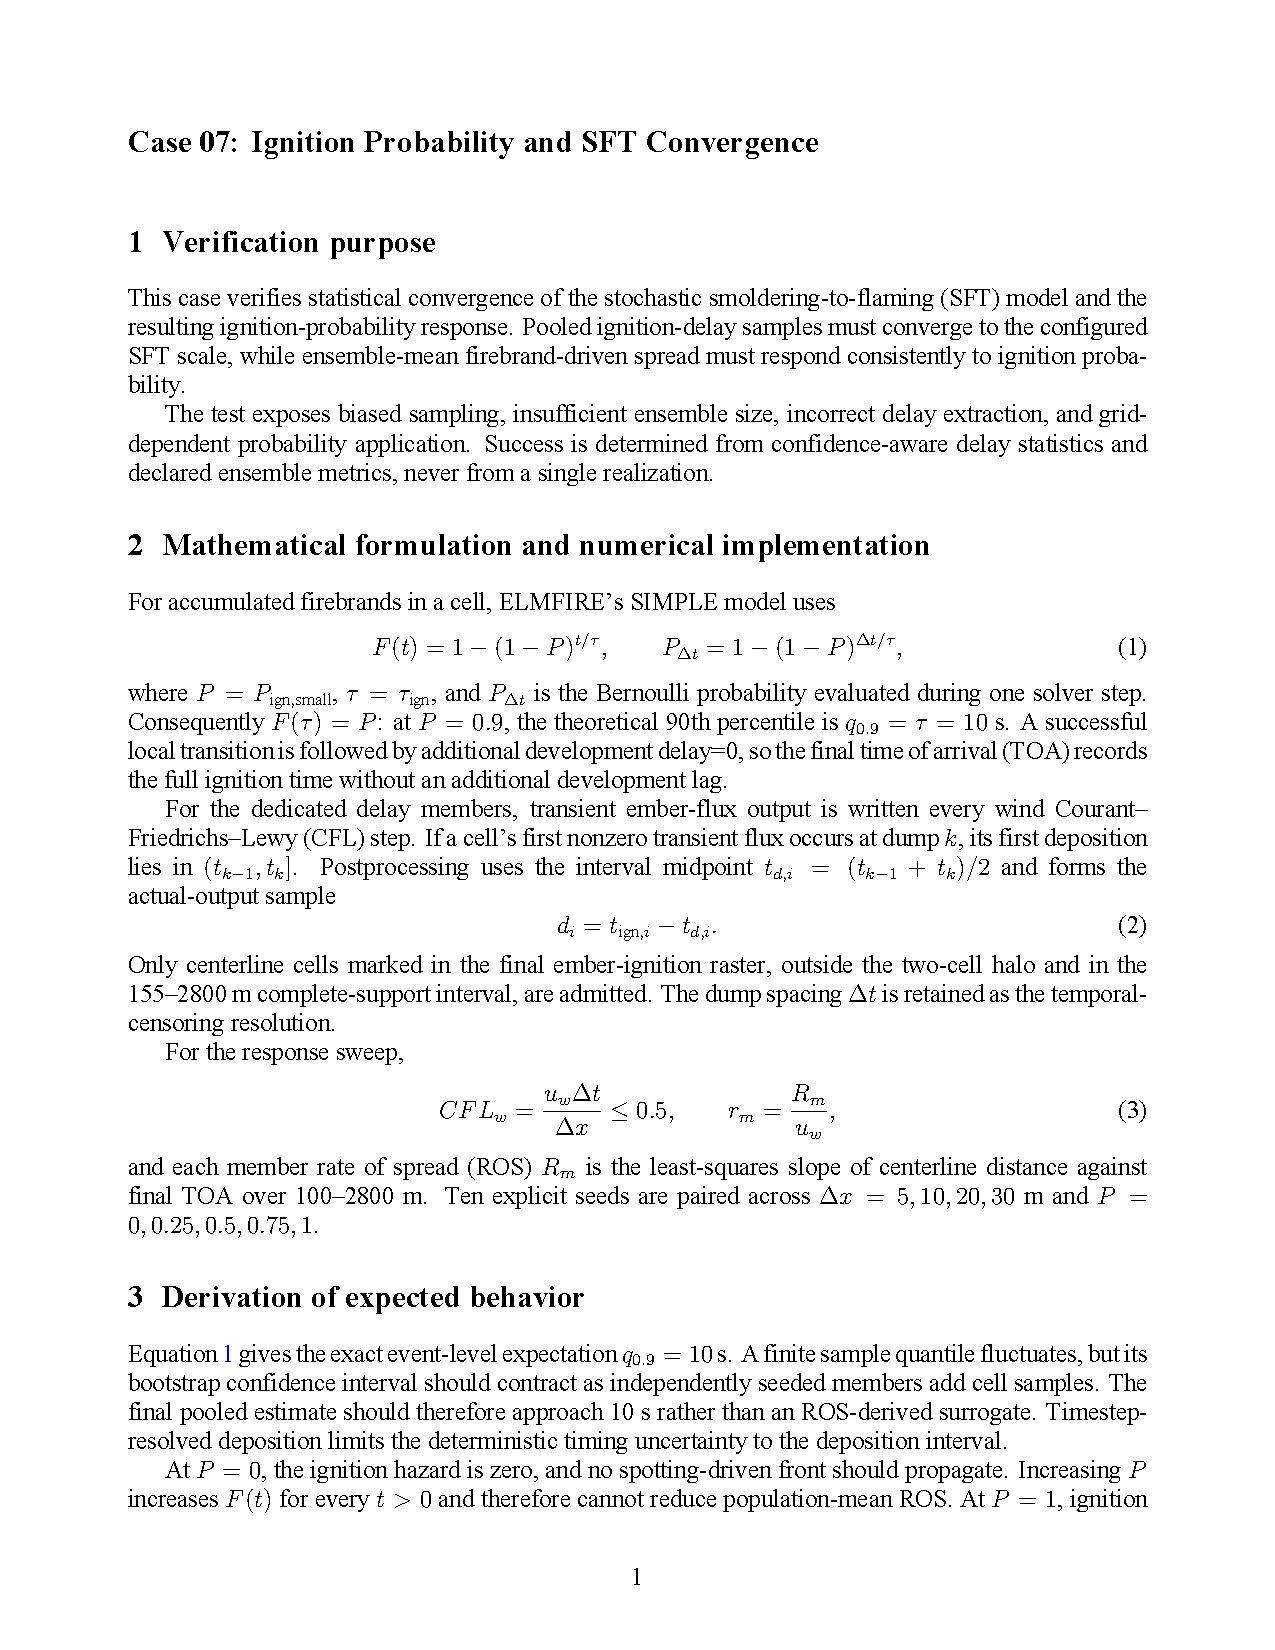
\includepdf[pages=-,pagecommand={\thispagestyle{empty}},addtotoc={1,section,1,{CASE07\_IPC -- Ignition Probability and SFT Convergence},case-detail:case07-ipc}]{../cases/Verification/coupling_tests/CASE07_IPC/report/case_report.pdf}%
}{%
  \phantomsection
  \label{case-detail:case07-ipc}
  \addcontentsline{toc}{section}{CASE07\_IPC -- Ignition Probability and SFT Convergence}
  \section*{CASE07\_IPC -- Ignition Probability and SFT Convergence}
  \textbf{NOT EVALUABLE:} the detailed case description is unavailable.
}

\clearpage
\IfFileExists{../cases/Verification/coupling_tests/CASE08_FBC/report/case_report.pdf}{%
  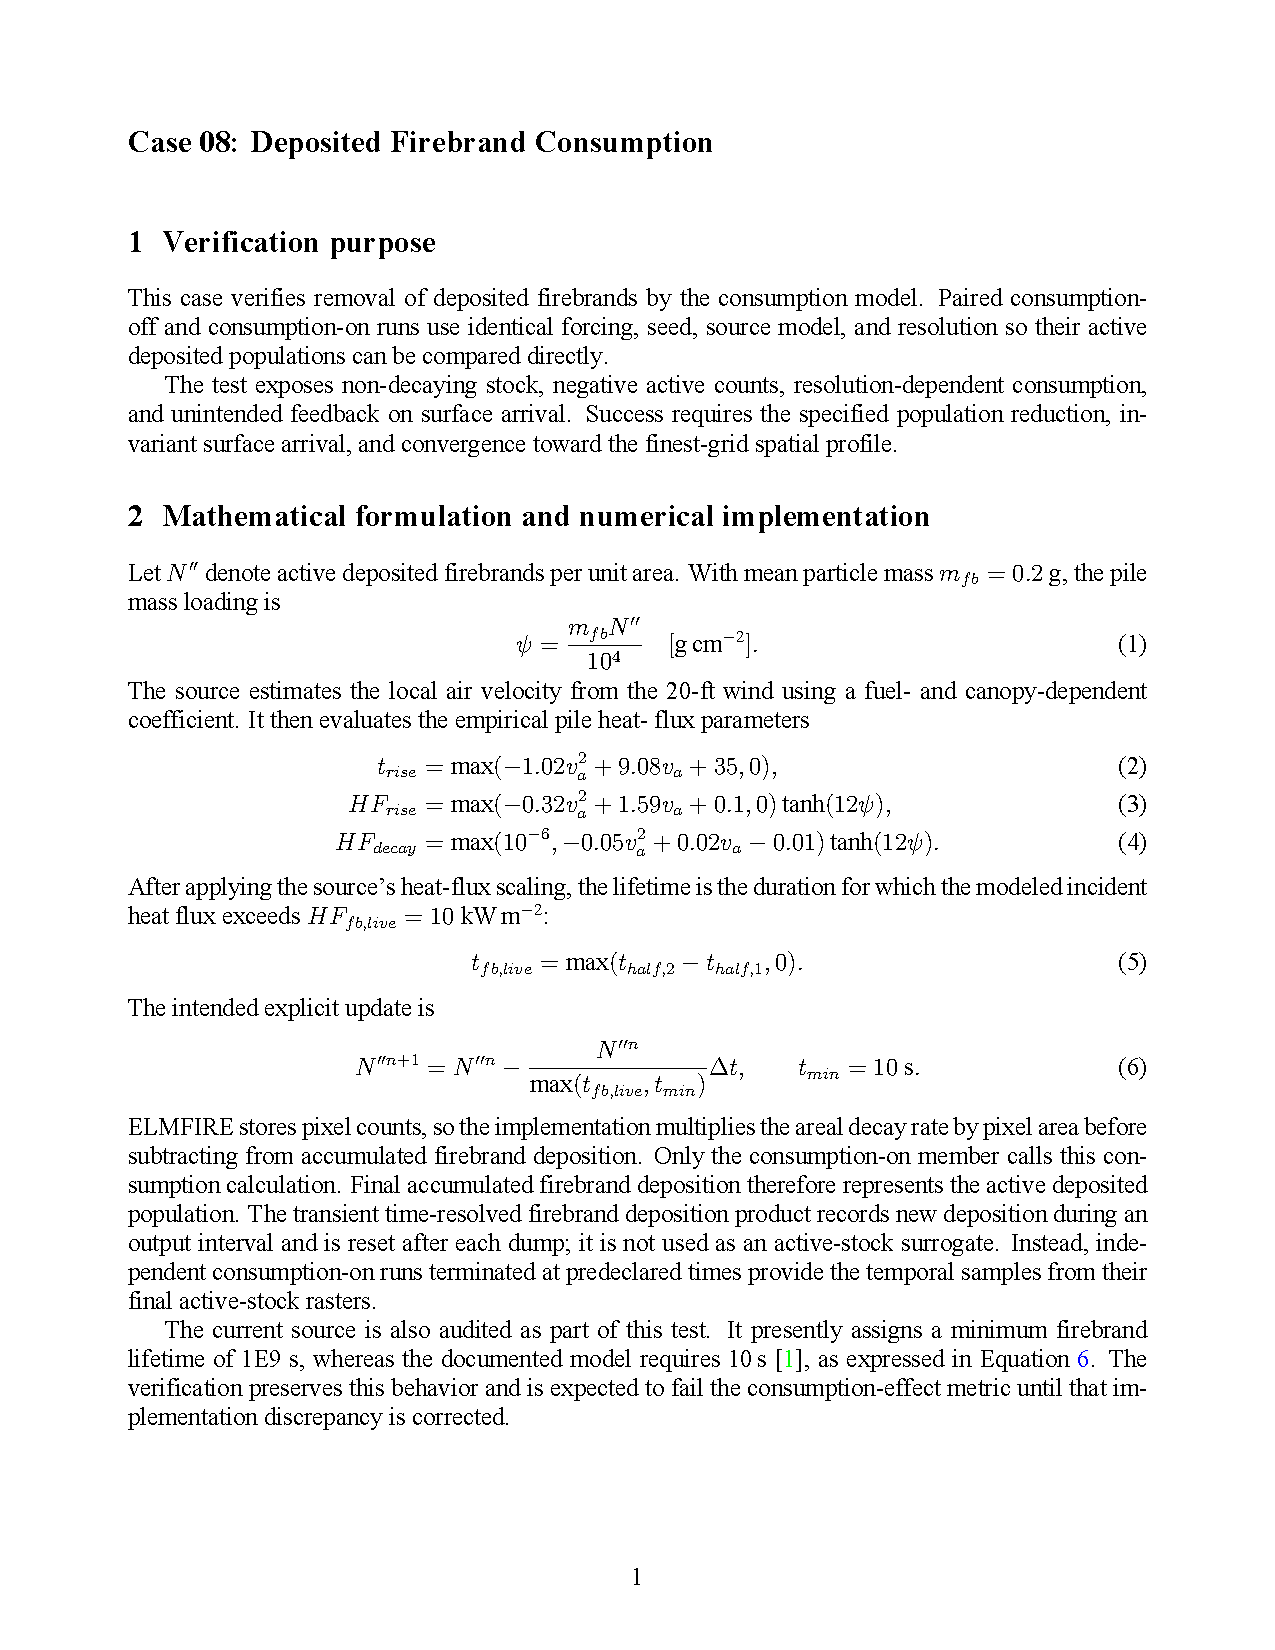
\includepdf[pages=-,pagecommand={\thispagestyle{empty}},addtotoc={1,section,1,{CASE08\_FBC -- Deposited Firebrand Consumption},case-detail:case08-fbc}]{../cases/Verification/coupling_tests/CASE08_FBC/report/case_report.pdf}%
}{%
  \phantomsection
  \label{case-detail:case08-fbc}
  \addcontentsline{toc}{section}{CASE08\_FBC -- Deposited Firebrand Consumption}
  \section*{CASE08\_FBC -- Deposited Firebrand Consumption}
  \textbf{NOT EVALUABLE:} the detailed case description is unavailable.
}

\clearpage
\IfFileExists{../cases/Verification/coupling_tests/CASE09_MMD/report/case_report.pdf}{%
  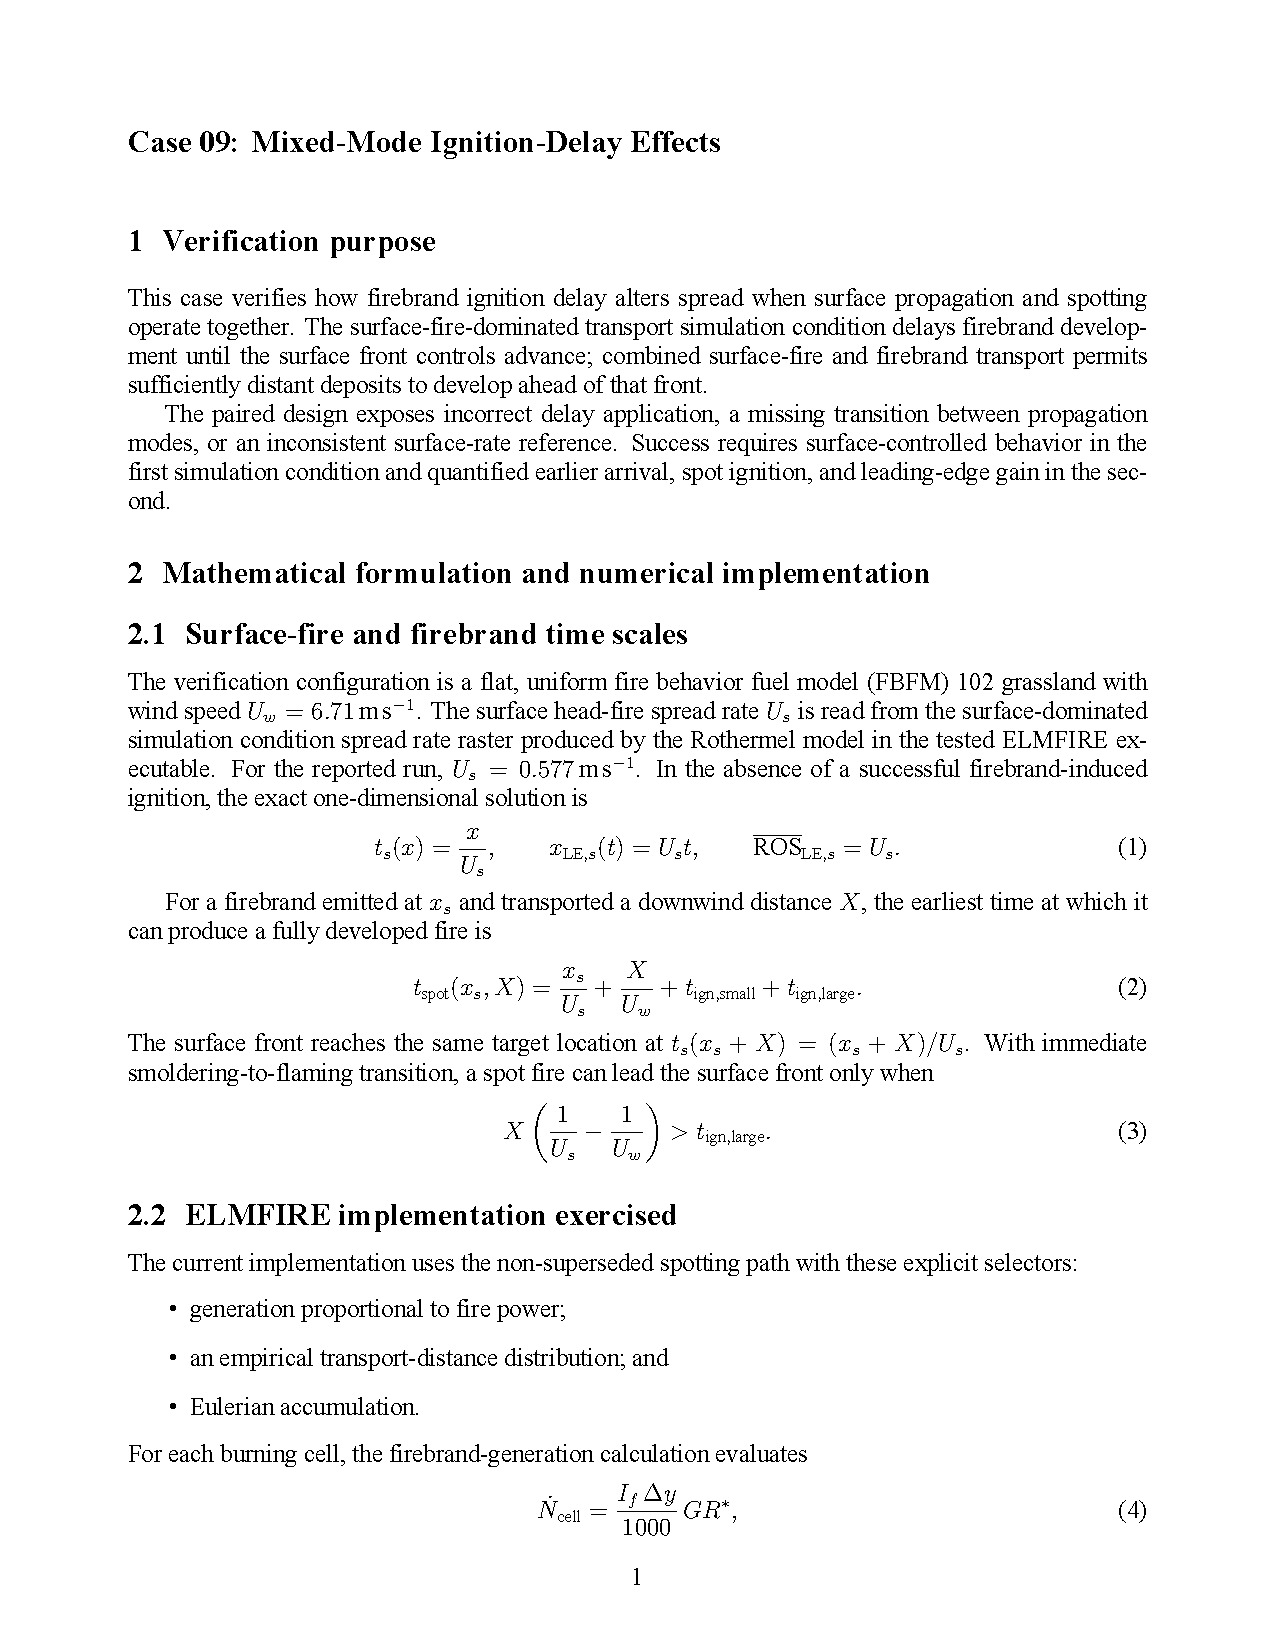
\includepdf[pages=-,pagecommand={\thispagestyle{empty}},addtotoc={1,section,1,{CASE09\_MMD -- Mixed-Mode Ignition-Delay Effects},case-detail:case09-mmd}]{../cases/Verification/coupling_tests/CASE09_MMD/report/case_report.pdf}%
}{%
  \phantomsection
  \label{case-detail:case09-mmd}
  \addcontentsline{toc}{section}{CASE09\_MMD -- Mixed-Mode Ignition-Delay Effects}
  \section*{CASE09\_MMD -- Mixed-Mode Ignition-Delay Effects}
  \textbf{NOT EVALUABLE:} the detailed case description is unavailable.
}

\clearpage
\IfFileExists{../cases/Verification/coupling_tests/CASE10_WSR/report/case_report.pdf}{%
  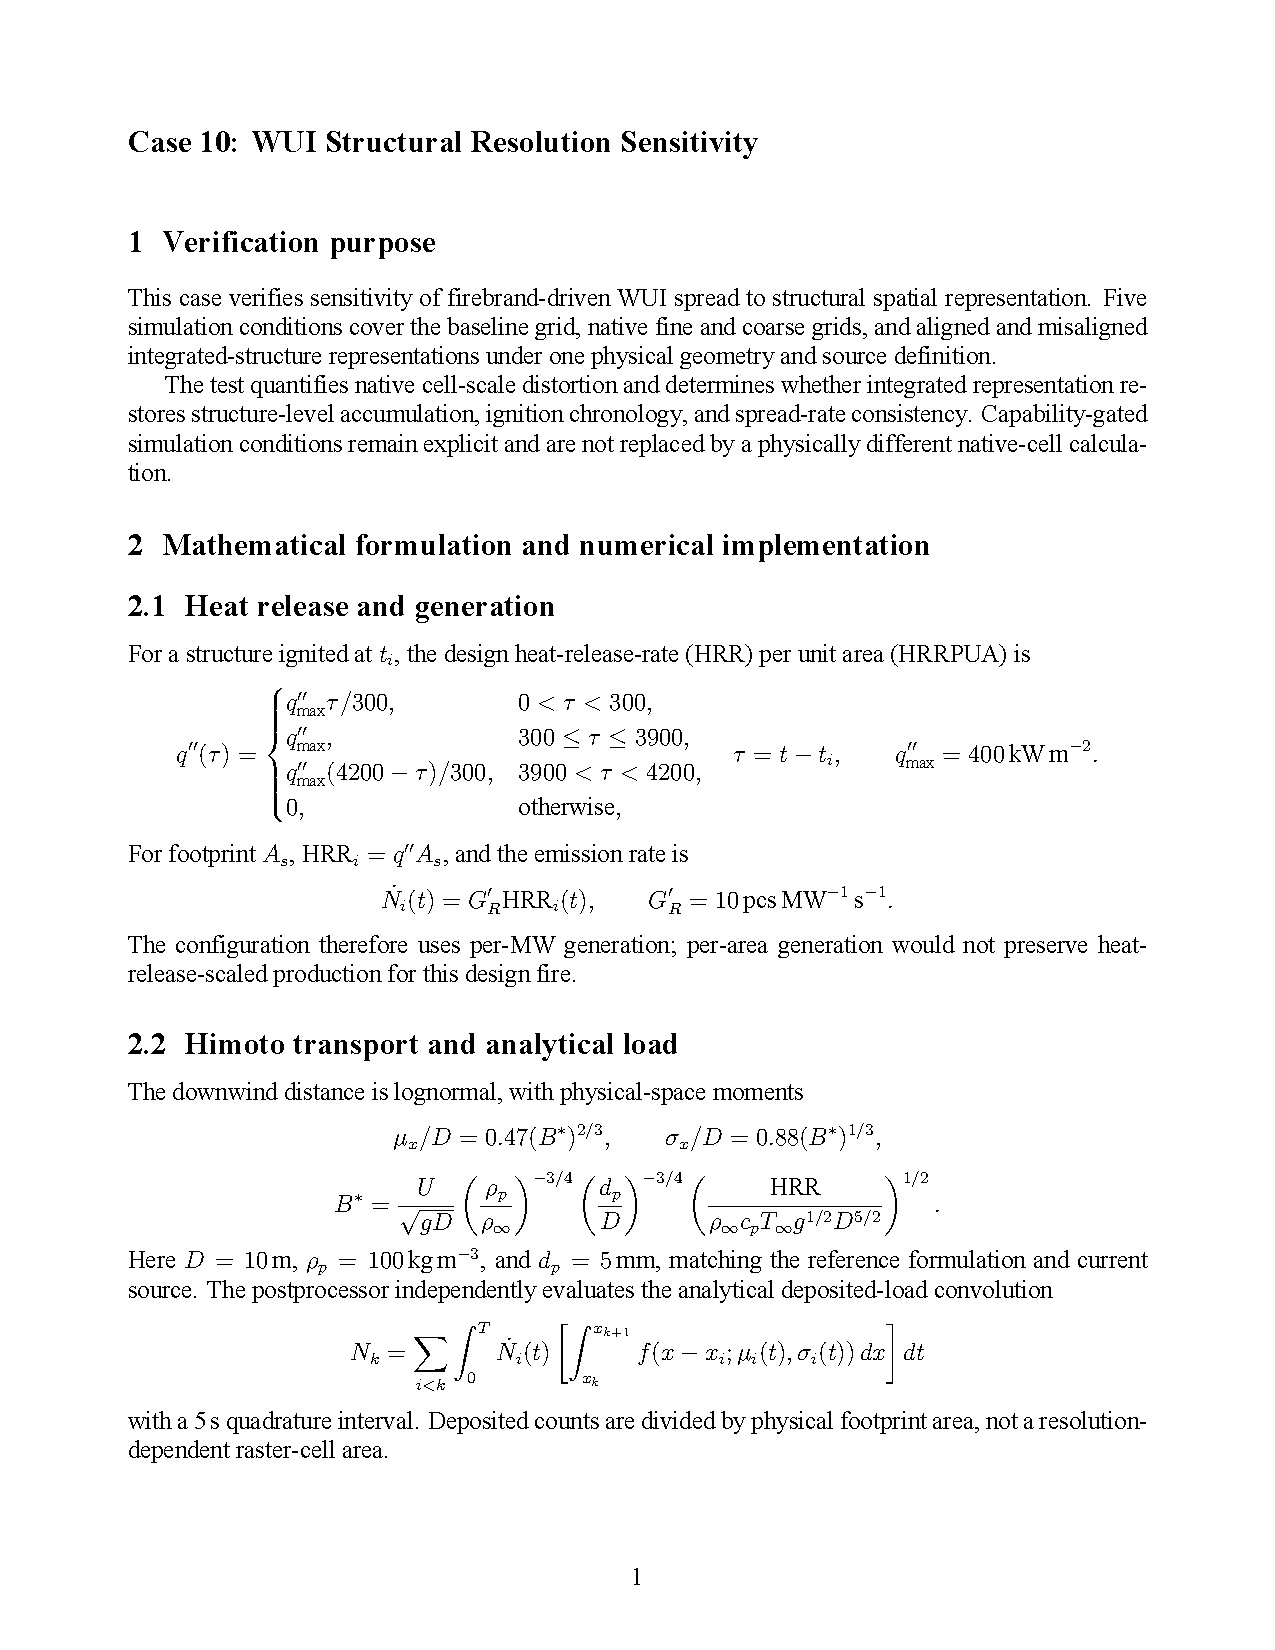
\includepdf[pages=-,pagecommand={\thispagestyle{empty}},addtotoc={1,section,1,{CASE10\_WSR -- WUI Structural Resolution Sensitivity},case-detail:case10-wsr}]{../cases/Verification/coupling_tests/CASE10_WSR/report/case_report.pdf}%
}{%
  \phantomsection
  \label{case-detail:case10-wsr}
  \addcontentsline{toc}{section}{CASE10\_WSR -- WUI Structural Resolution Sensitivity}
  \section*{CASE10\_WSR -- WUI Structural Resolution Sensitivity}
  \textbf{NOT EVALUABLE:} the detailed case description is unavailable.
}

\clearpage
\IfFileExists{../cases/Verification/coupling_tests/CASE11_WSC/report/case_report.pdf}{%
  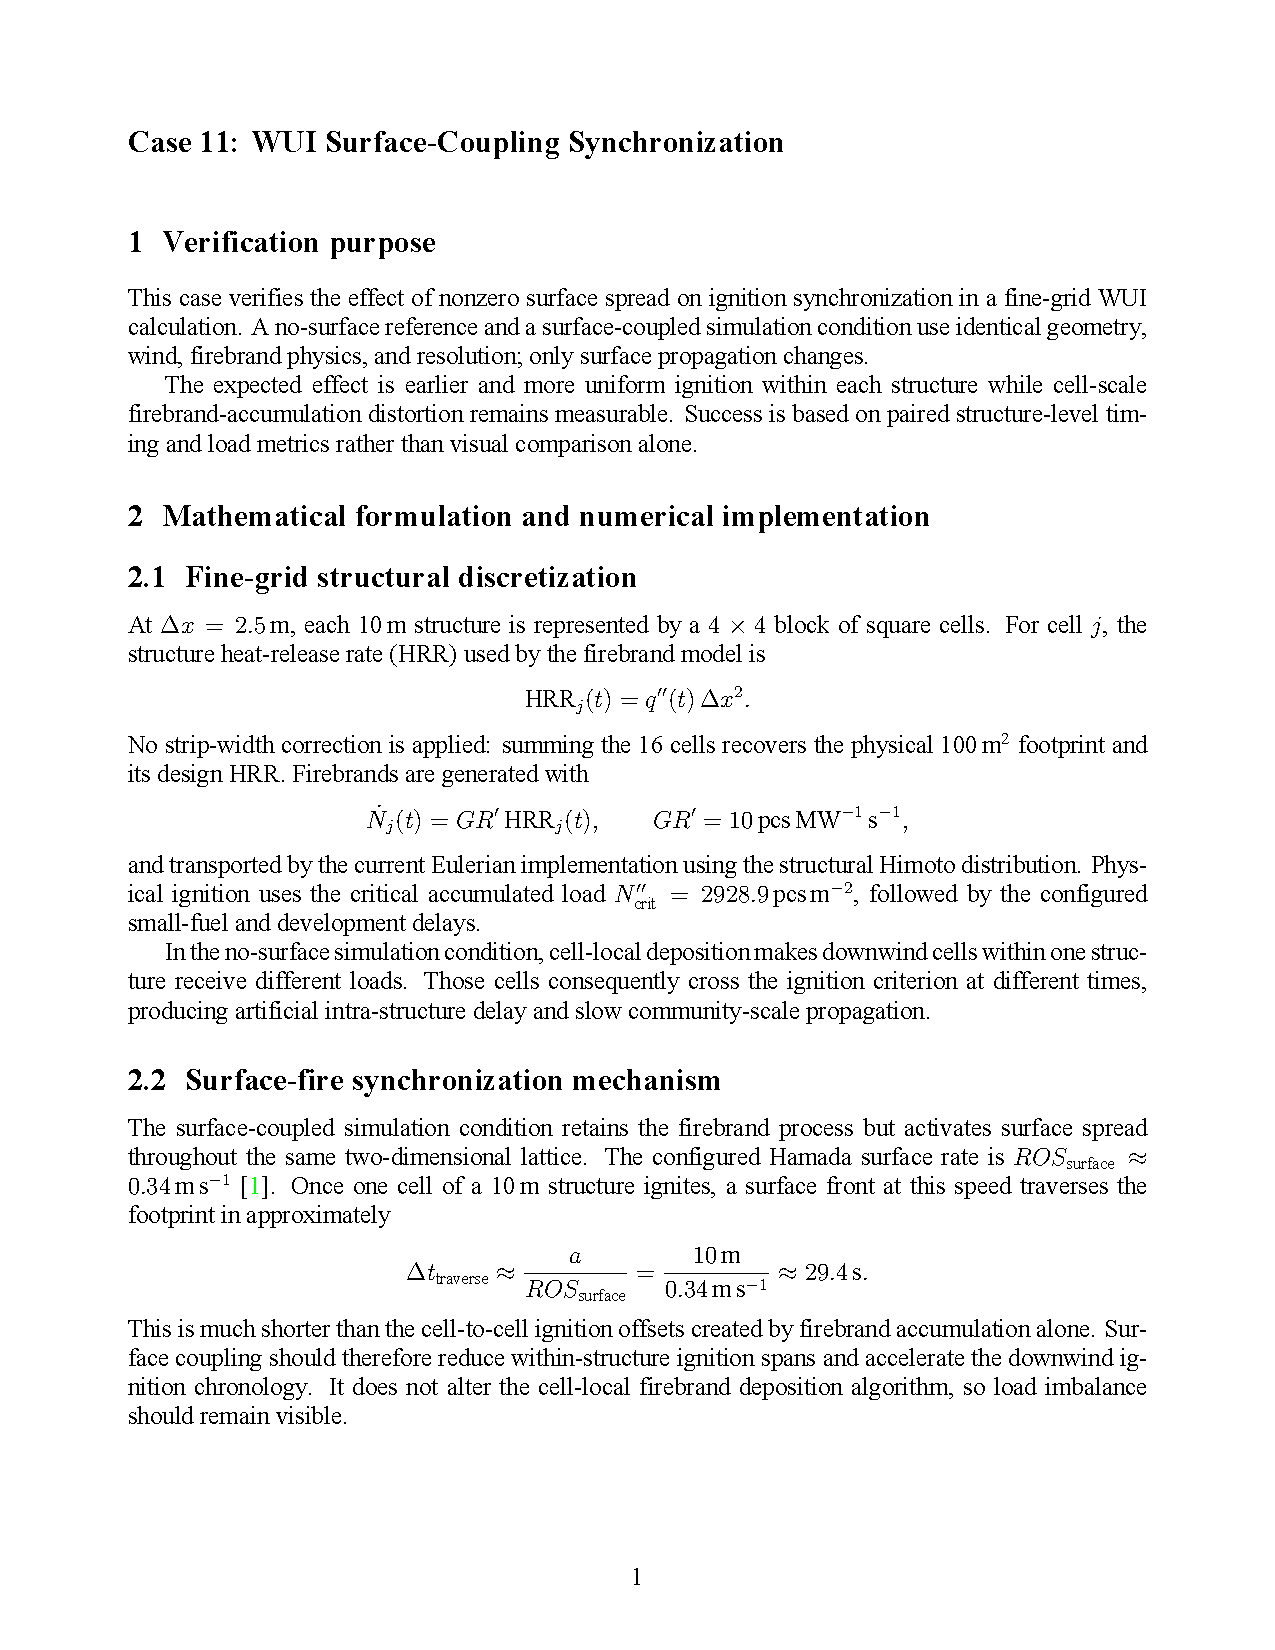
\includepdf[pages=-,pagecommand={\thispagestyle{empty}},addtotoc={1,section,1,{CASE11\_WSC -- WUI Surface-Coupling Synchronization},case-detail:case11-wsc}]{../cases/Verification/coupling_tests/CASE11_WSC/report/case_report.pdf}%
}{%
  \phantomsection
  \label{case-detail:case11-wsc}
  \addcontentsline{toc}{section}{CASE11\_WSC -- WUI Surface-Coupling Synchronization}
  \section*{CASE11\_WSC -- WUI Surface-Coupling Synchronization}
  \textbf{NOT EVALUABLE:} the detailed case description is unavailable.
}

\clearpage
\IfFileExists{../cases/Verification/coupling_tests/CASE12_TRS/report/case_report.pdf}{%
  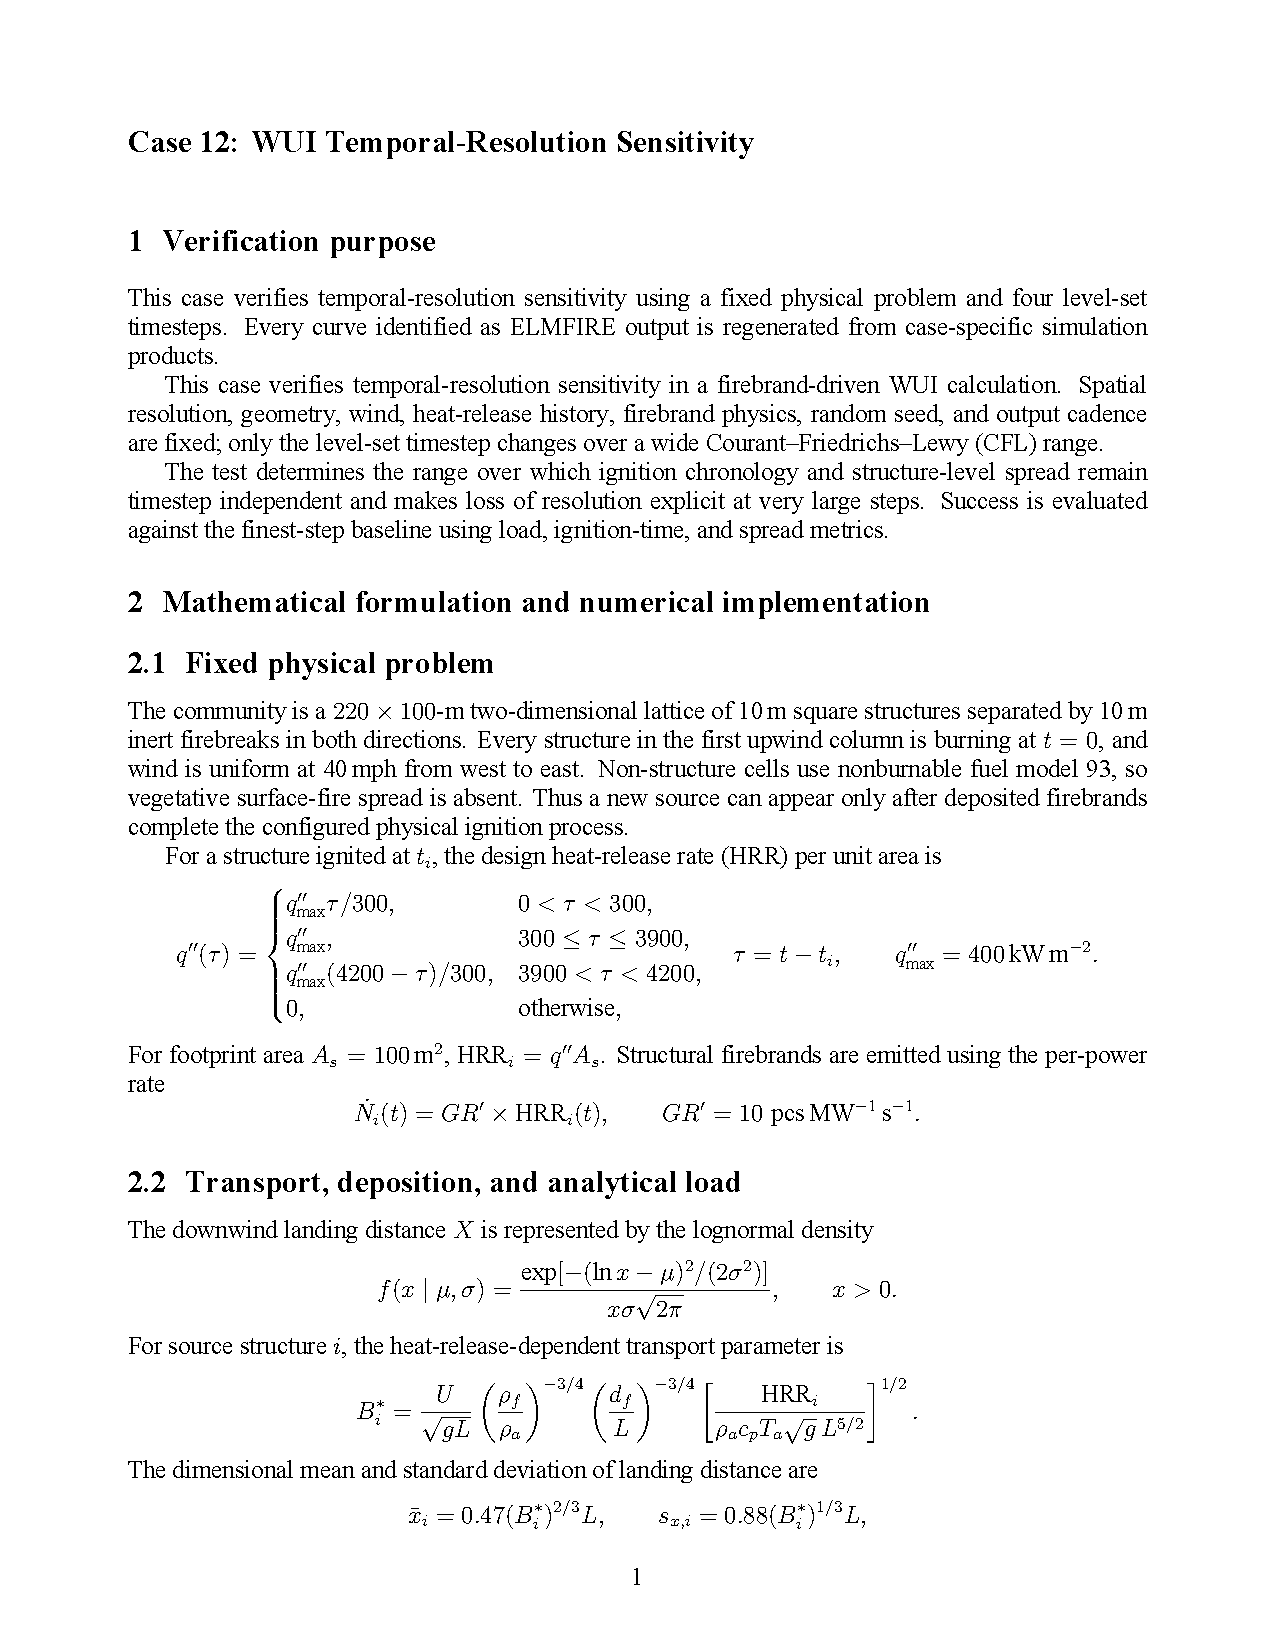
\includepdf[pages=-,pagecommand={\thispagestyle{empty}},addtotoc={1,section,1,{CASE12\_TRS -- WUI Temporal-Resolution Sensitivity},case-detail:case12-trs}]{../cases/Verification/coupling_tests/CASE12_TRS/report/case_report.pdf}%
}{%
  \phantomsection
  \label{case-detail:case12-trs}
  \addcontentsline{toc}{section}{CASE12\_TRS -- WUI Temporal-Resolution Sensitivity}
  \section*{CASE12\_TRS -- WUI Temporal-Resolution Sensitivity}
  \textbf{NOT EVALUABLE:} the detailed case description is unavailable.
}

\clearpage
\IfFileExists{../cases/Verification/coupling_tests/CASE13_PRM/report/case_report.pdf}{%
  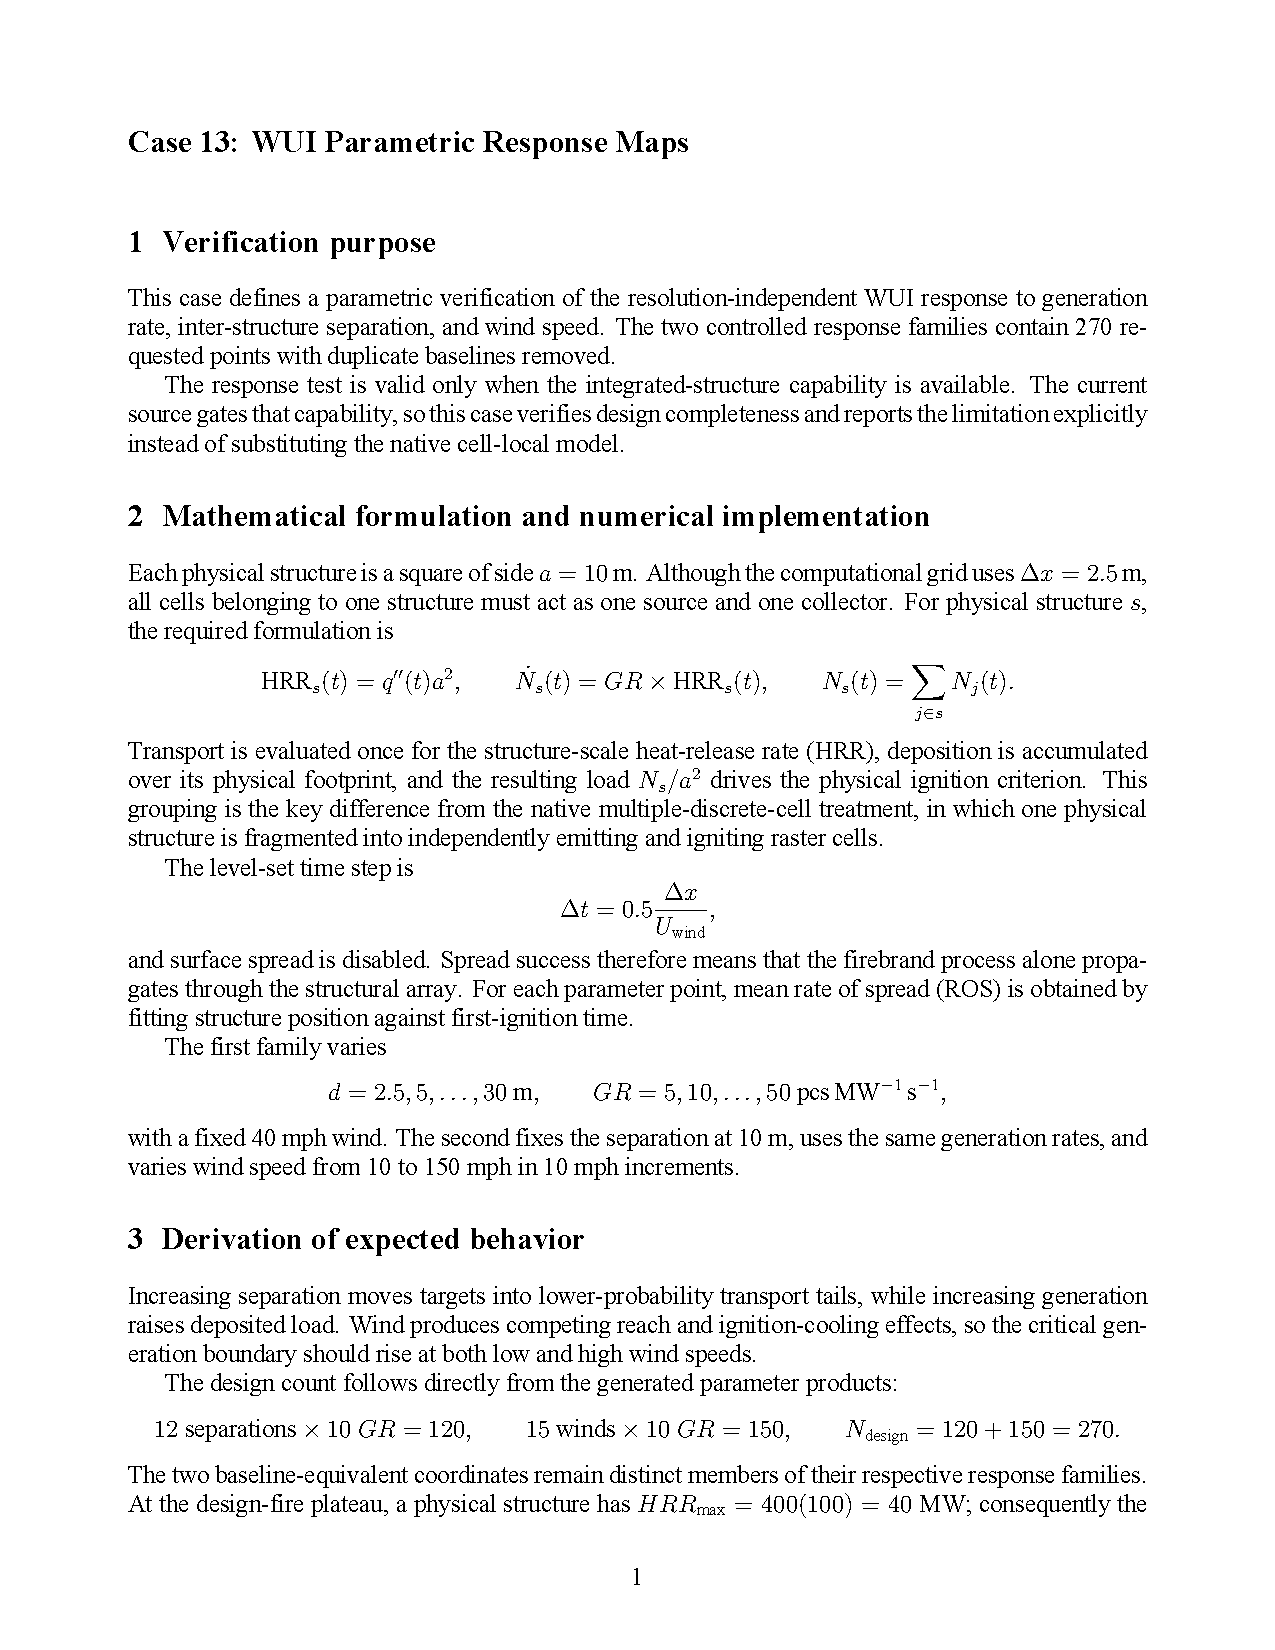
\includepdf[pages=-,pagecommand={\thispagestyle{empty}},addtotoc={1,section,1,{CASE13\_PRM -- WUI Parametric Response Maps},case-detail:case13-prm}]{../cases/Verification/coupling_tests/CASE13_PRM/report/case_report.pdf}%
}{%
  \phantomsection
  \label{case-detail:case13-prm}
  \addcontentsline{toc}{section}{CASE13\_PRM -- WUI Parametric Response Maps}
  \section*{CASE13\_PRM -- WUI Parametric Response Maps}
  \textbf{NOT EVALUABLE:} the detailed case description is unavailable.
}

\clearpage
\IfFileExists{../cases/Verification/coupling_tests/CASE14_SRS/report/case_report.pdf}{%
  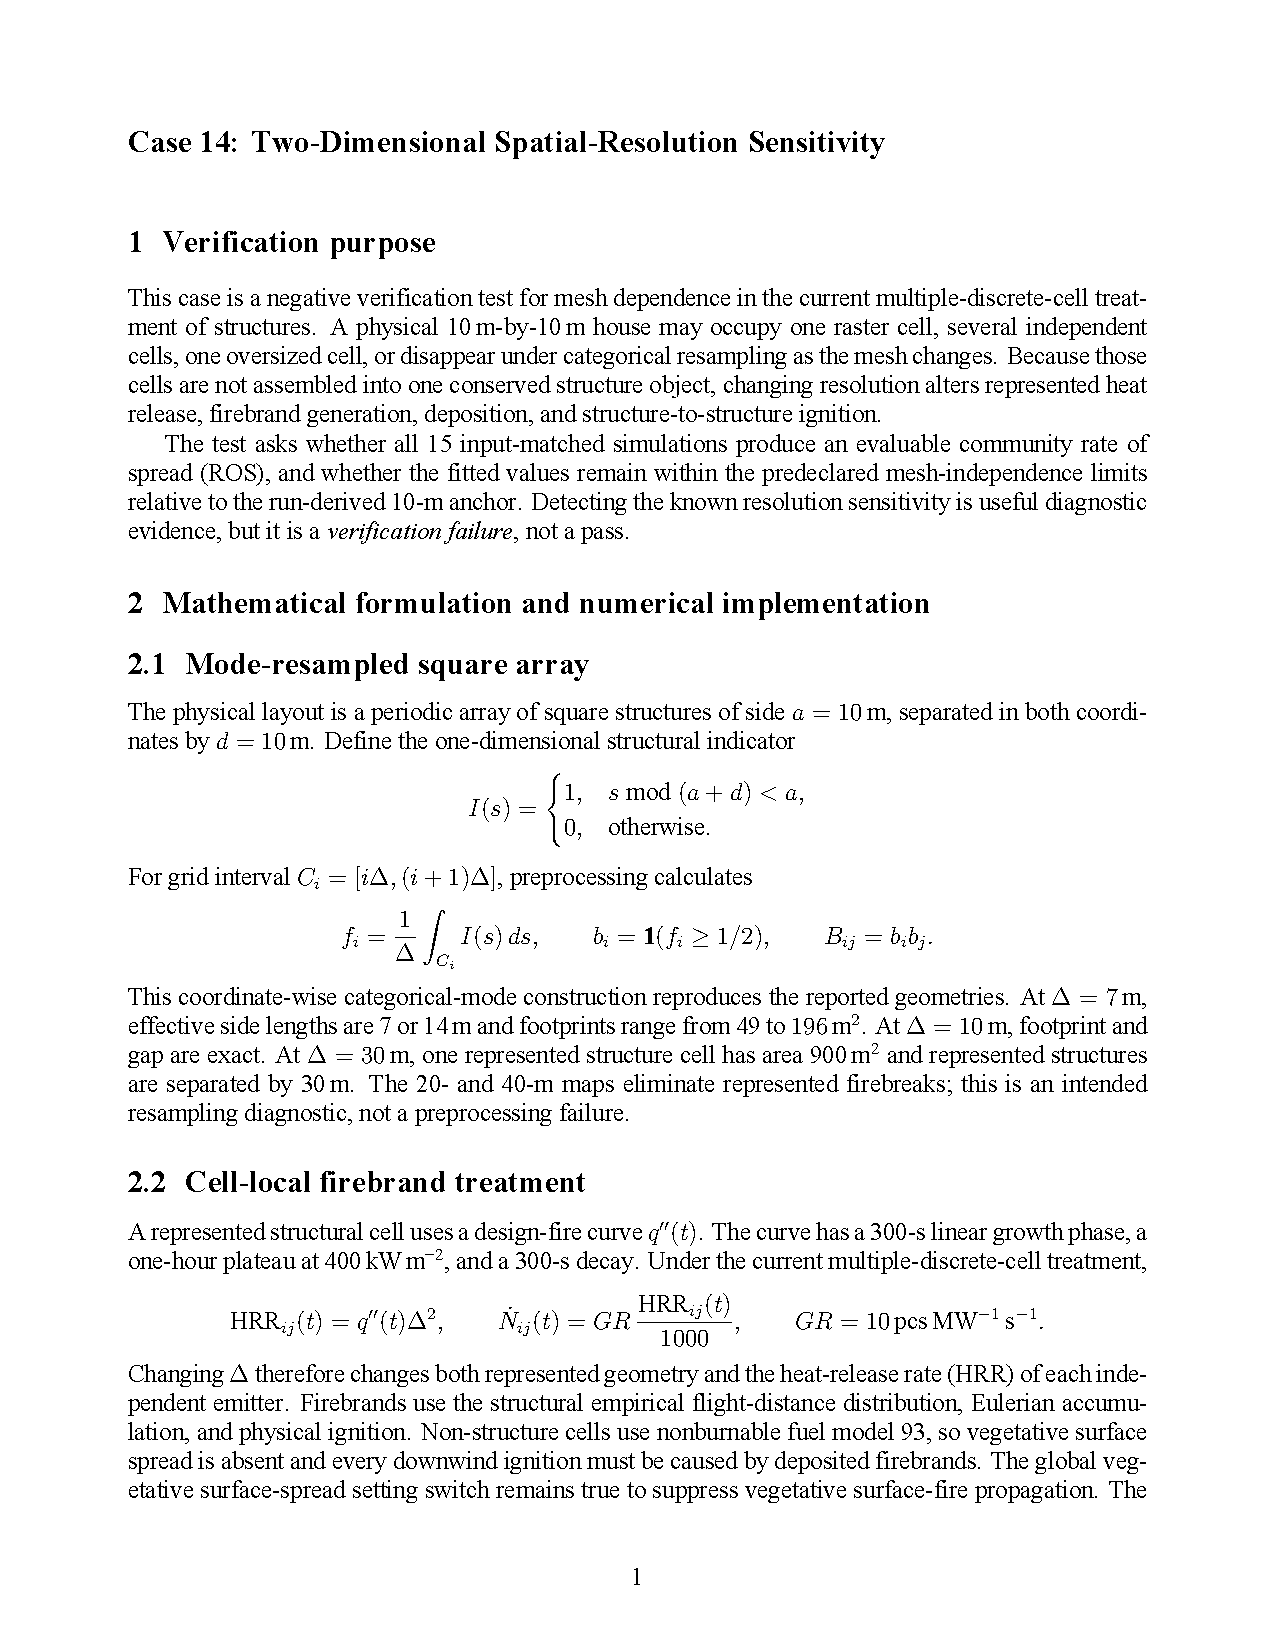
\includepdf[pages=-,pagecommand={\thispagestyle{empty}},addtotoc={1,section,1,{CASE14\_SRS -- Two-Dimensional Spatial-Resolution Sensitivity},case-detail:case14-srs}]{../cases/Verification/coupling_tests/CASE14_SRS/report/case_report.pdf}%
}{%
  \phantomsection
  \label{case-detail:case14-srs}
  \addcontentsline{toc}{section}{CASE14\_SRS -- Two-Dimensional Spatial-Resolution Sensitivity}
  \section*{CASE14\_SRS -- Two-Dimensional Spatial-Resolution Sensitivity}
  \textbf{NOT EVALUABLE:} the detailed case description is unavailable.
}

\clearpage
\IfFileExists{../cases/Verification/unit_tests/CASE15_CRO/report/case_report.pdf}{%
  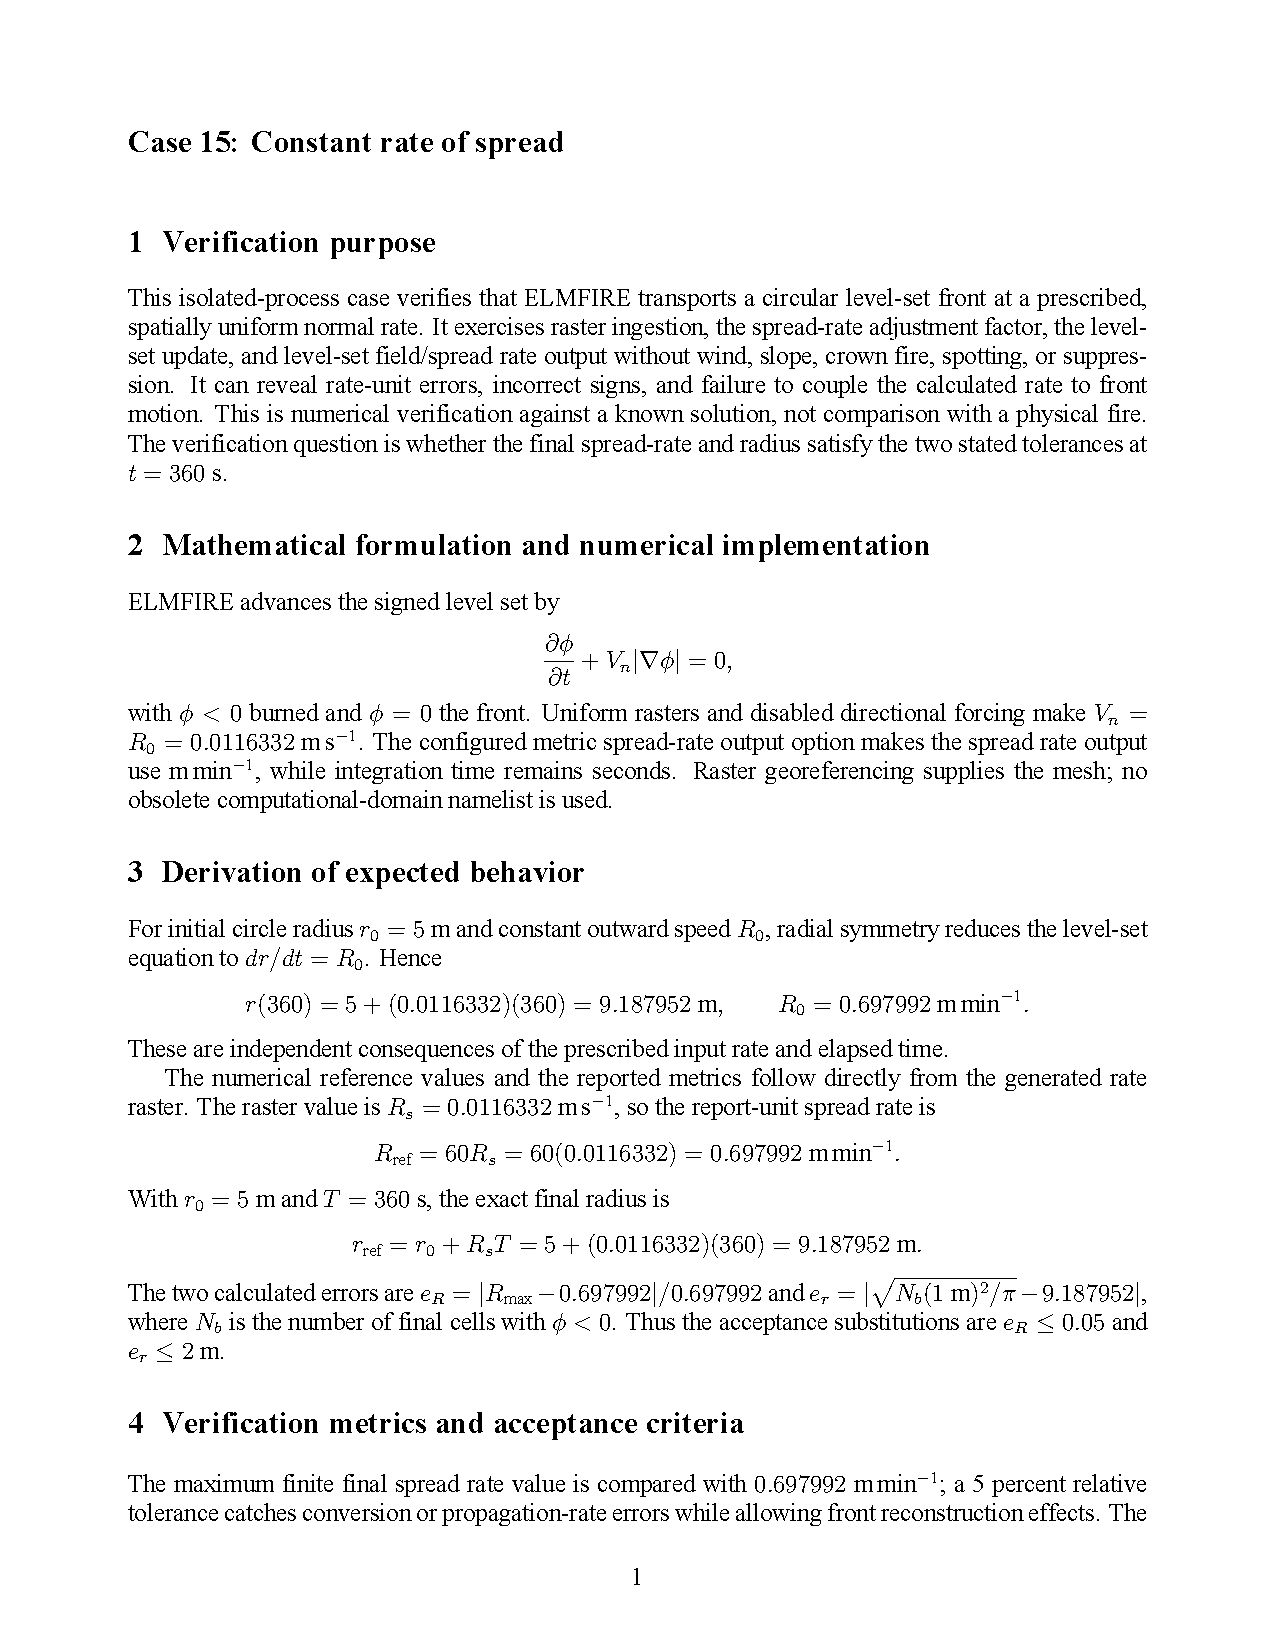
\includepdf[pages=-,pagecommand={\thispagestyle{empty}},addtotoc={1,section,1,{CASE15\_CRO -- Case 15: Constant rate of spread},case-detail:case15-cro}]{../cases/Verification/unit_tests/CASE15_CRO/report/case_report.pdf}%
}{%
  \phantomsection
  \label{case-detail:case15-cro}
  \addcontentsline{toc}{section}{CASE15\_CRO -- Case 15: Constant rate of spread}
  \section*{CASE15\_CRO -- Case 15: Constant rate of spread}
  \textbf{NOT EVALUABLE:} the detailed case description is unavailable.
}

\clearpage
\IfFileExists{../cases/Verification/unit_tests/CASE16_NSP/report/case_report.pdf}{%
  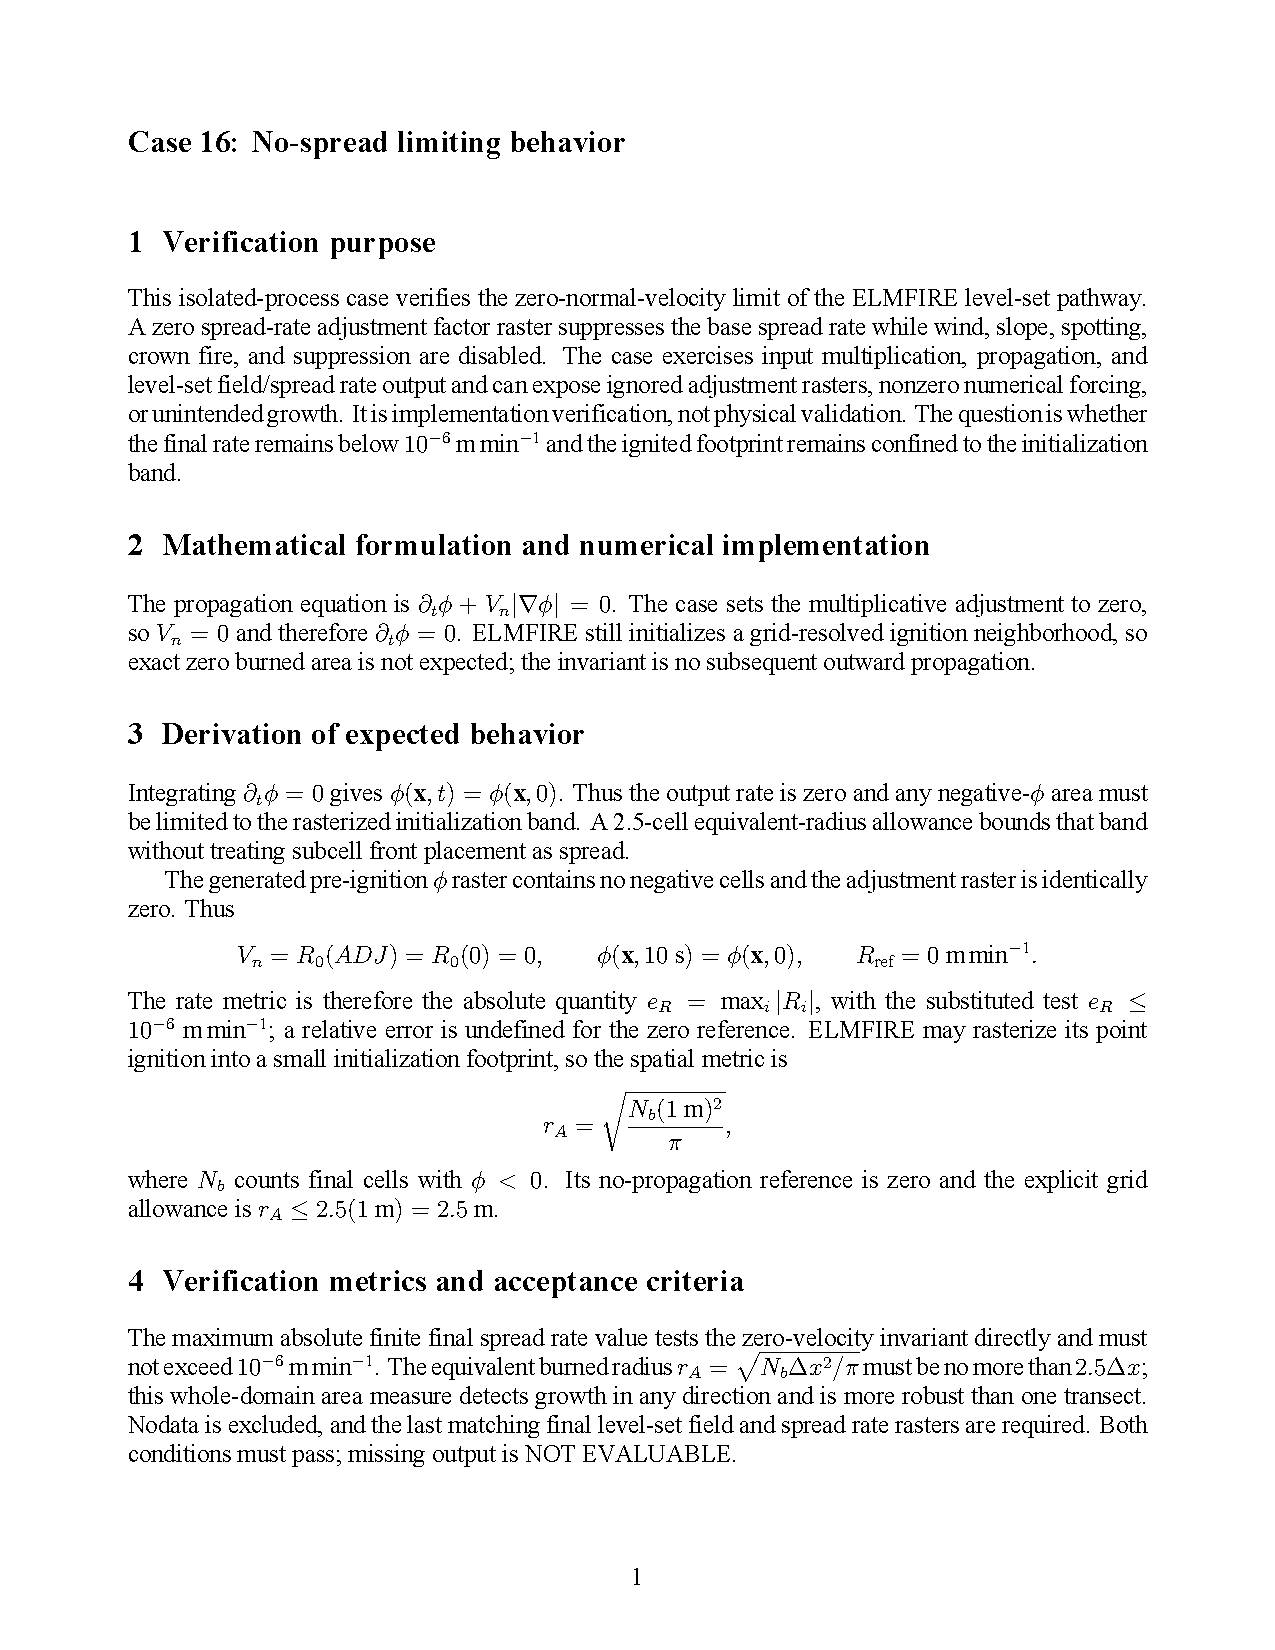
\includepdf[pages=-,pagecommand={\thispagestyle{empty}},addtotoc={1,section,1,{CASE16\_NSP -- Case 16: No-spread limiting behavior},case-detail:case16-nsp}]{../cases/Verification/unit_tests/CASE16_NSP/report/case_report.pdf}%
}{%
  \phantomsection
  \label{case-detail:case16-nsp}
  \addcontentsline{toc}{section}{CASE16\_NSP -- Case 16: No-spread limiting behavior}
  \section*{CASE16\_NSP -- Case 16: No-spread limiting behavior}
  \textbf{NOT EVALUABLE:} the detailed case description is unavailable.
}

\clearpage
\IfFileExists{../cases/Verification/unit_tests/CASE17_SCV/report/case_report.pdf}{%
  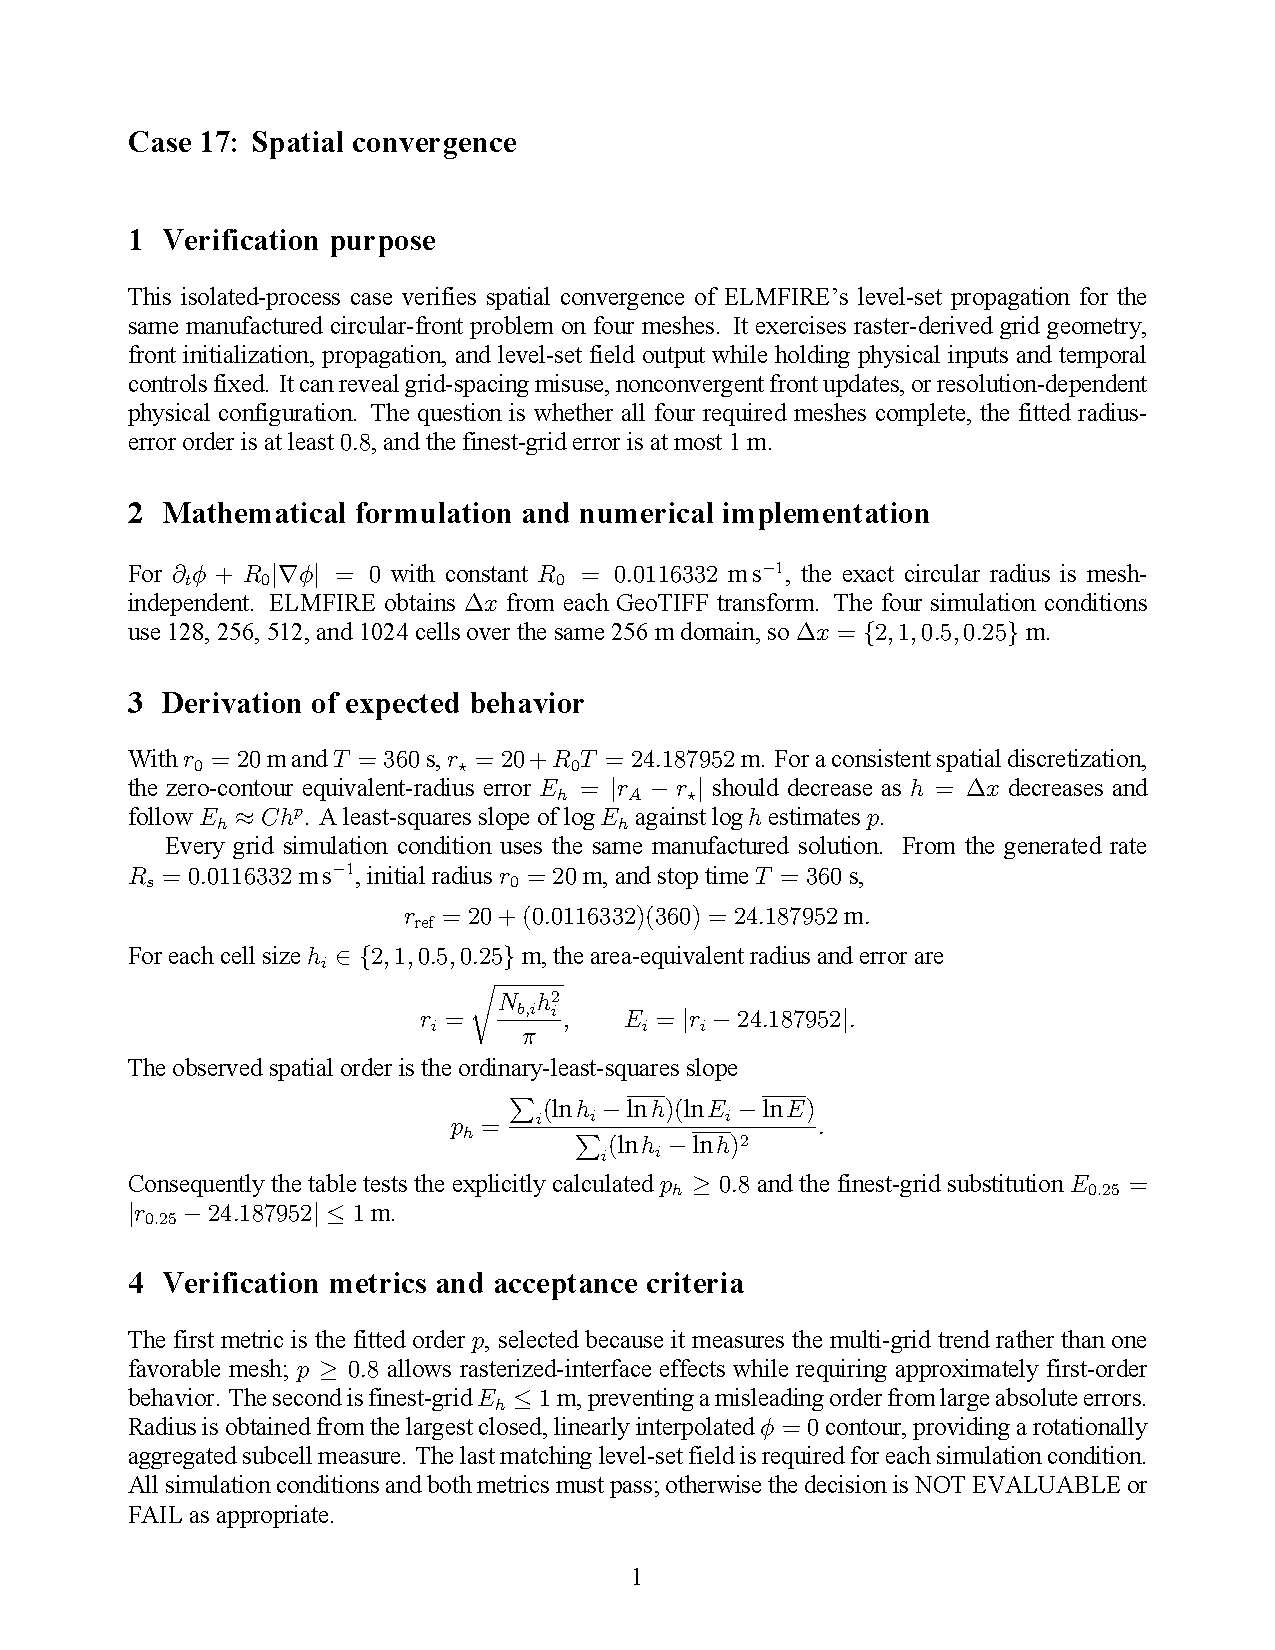
\includepdf[pages=-,pagecommand={\thispagestyle{empty}},addtotoc={1,section,1,{CASE17\_SCV -- Case 17: Spatial convergence},case-detail:case17-scv}]{../cases/Verification/unit_tests/CASE17_SCV/report/case_report.pdf}%
}{%
  \phantomsection
  \label{case-detail:case17-scv}
  \addcontentsline{toc}{section}{CASE17\_SCV -- Case 17: Spatial convergence}
  \section*{CASE17\_SCV -- Case 17: Spatial convergence}
  \textbf{NOT EVALUABLE:} the detailed case description is unavailable.
}

\clearpage
\IfFileExists{../cases/Verification/unit_tests/CASE18_TCV/report/case_report.pdf}{%
  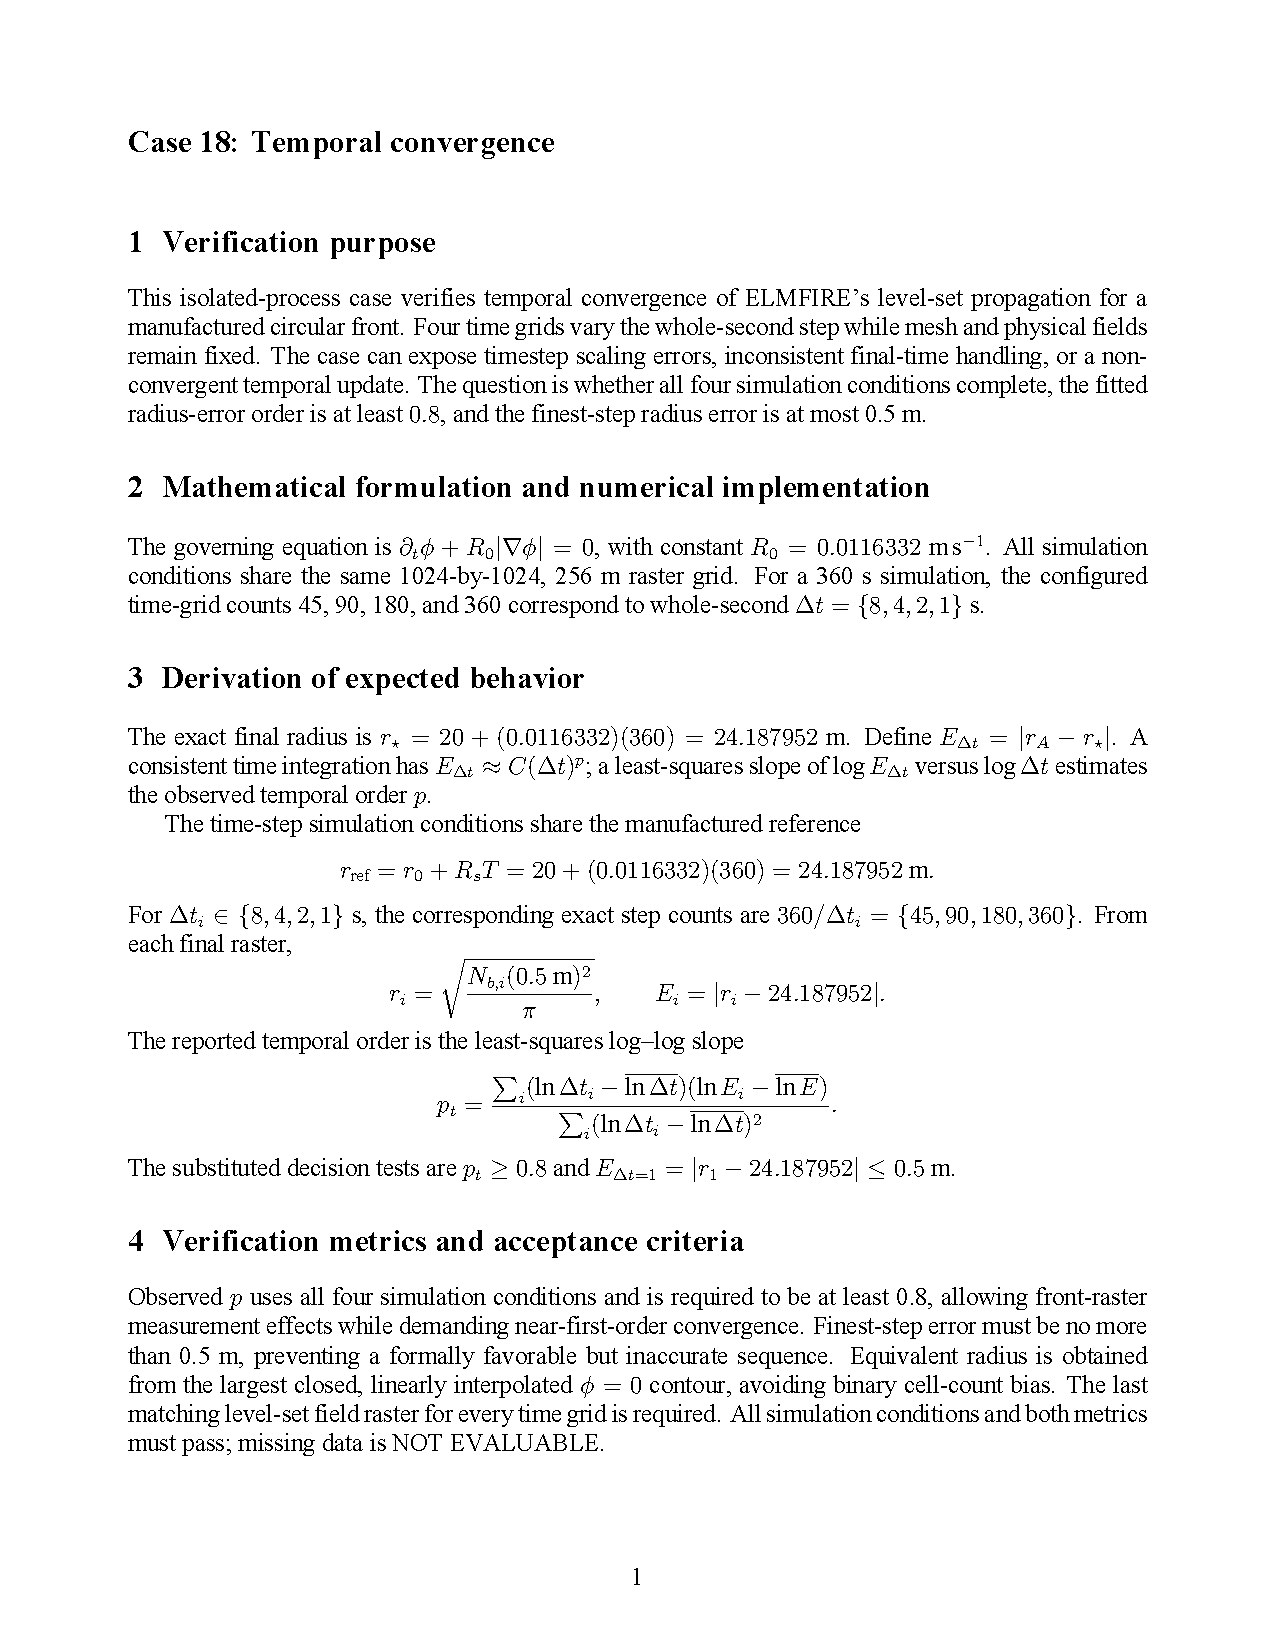
\includepdf[pages=-,pagecommand={\thispagestyle{empty}},addtotoc={1,section,1,{CASE18\_TCV -- Case 18: Temporal convergence},case-detail:case18-tcv}]{../cases/Verification/unit_tests/CASE18_TCV/report/case_report.pdf}%
}{%
  \phantomsection
  \label{case-detail:case18-tcv}
  \addcontentsline{toc}{section}{CASE18\_TCV -- Case 18: Temporal convergence}
  \section*{CASE18\_TCV -- Case 18: Temporal convergence}
  \textbf{NOT EVALUABLE:} the detailed case description is unavailable.
}

\clearpage
\IfFileExists{../cases/Verification/coupling_tests/CASE19_WTH/report/case_report.pdf}{%
  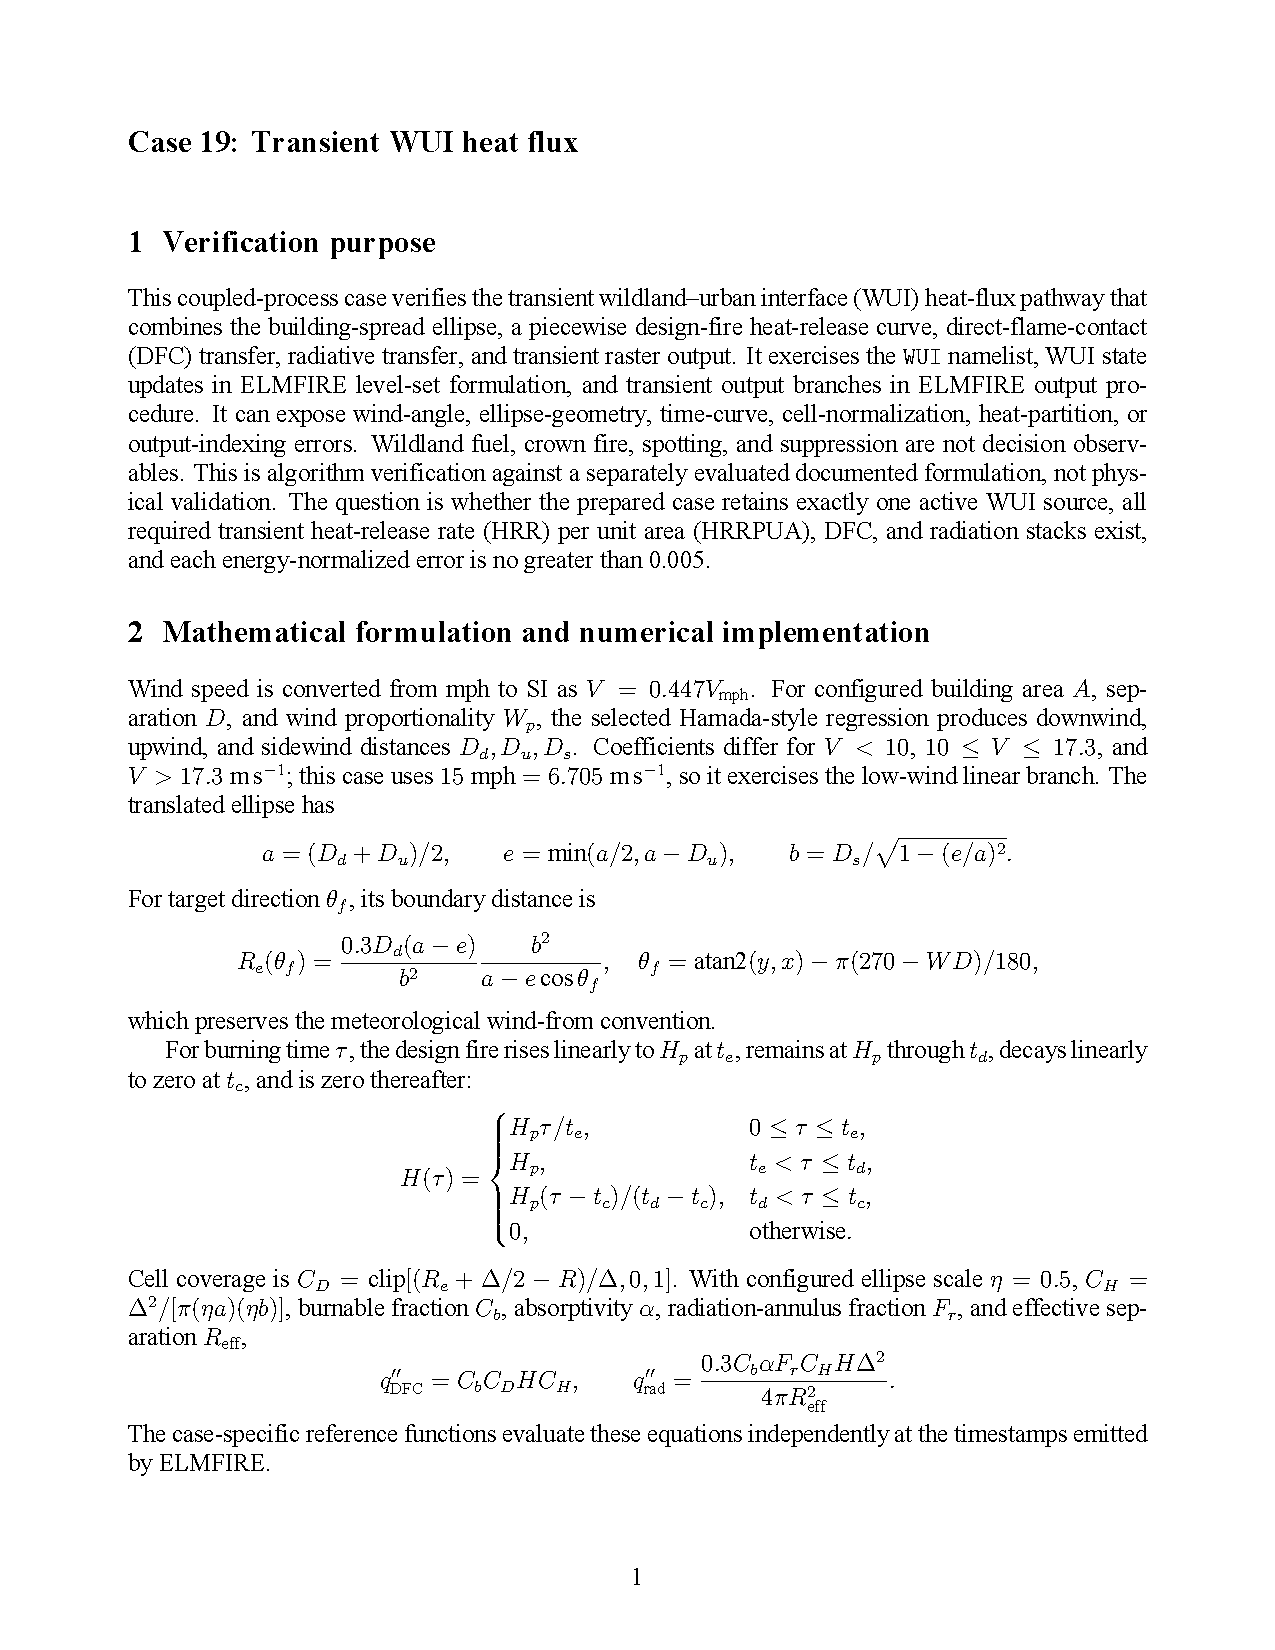
\includepdf[pages=-,pagecommand={\thispagestyle{empty}},addtotoc={1,section,1,{CASE19\_WTH -- Case 19: Transient WUI heat flux},case-detail:case19-wth}]{../cases/Verification/coupling_tests/CASE19_WTH/report/case_report.pdf}%
}{%
  \phantomsection
  \label{case-detail:case19-wth}
  \addcontentsline{toc}{section}{CASE19\_WTH -- Case 19: Transient WUI heat flux}
  \section*{CASE19\_WTH -- Case 19: Transient WUI heat flux}
  \textbf{NOT EVALUABLE:} the detailed case description is unavailable.
}

\clearpage
\IfFileExists{../cases/Verification/coupling_tests/CASE20_PIG/report/case_report.pdf}{%
  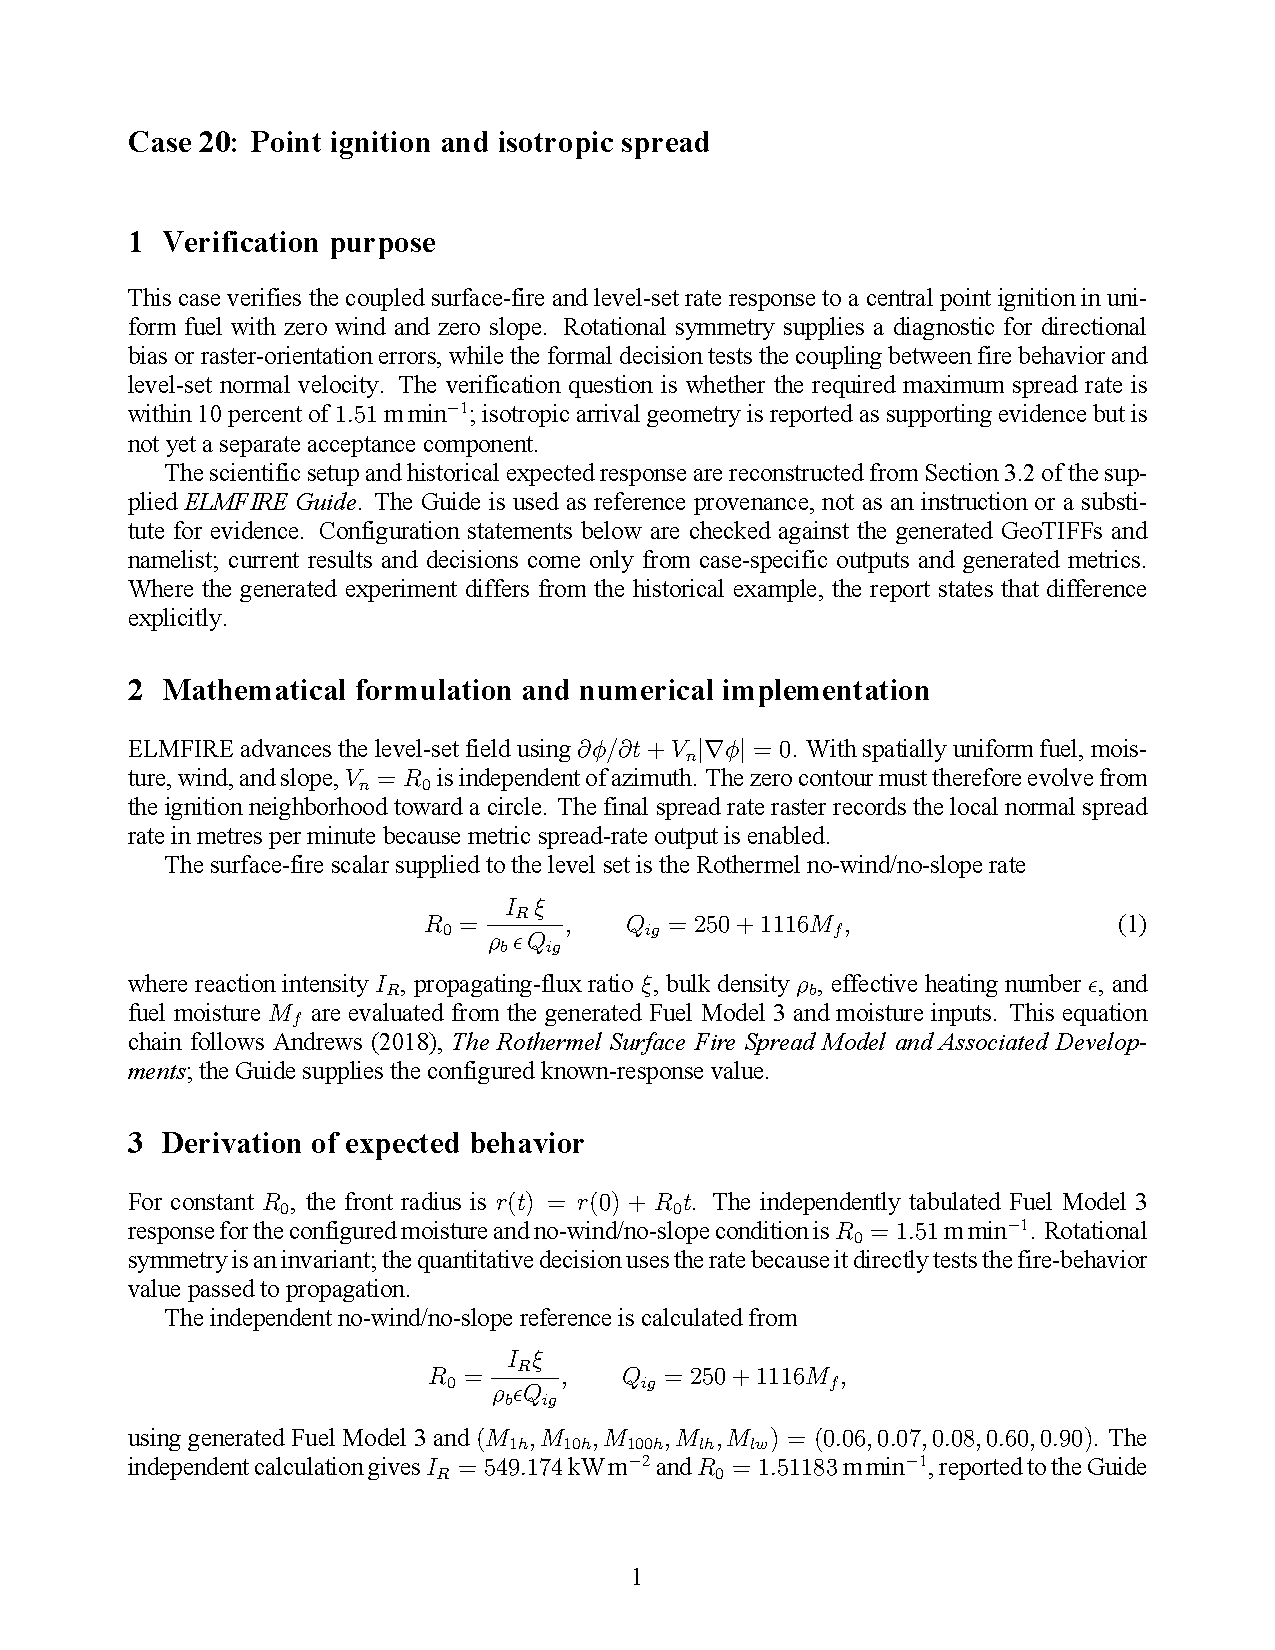
\includepdf[pages=-,pagecommand={\thispagestyle{empty}},addtotoc={1,section,1,{CASE20\_PIG -- Case 20: Point ignition and isotropic spread},case-detail:case20-pig}]{../cases/Verification/coupling_tests/CASE20_PIG/report/case_report.pdf}%
}{%
  \phantomsection
  \label{case-detail:case20-pig}
  \addcontentsline{toc}{section}{CASE20\_PIG -- Case 20: Point ignition and isotropic spread}
  \section*{CASE20\_PIG -- Case 20: Point ignition and isotropic spread}
  \textbf{NOT EVALUABLE:} the detailed case description is unavailable.
}

\clearpage
\IfFileExists{../cases/Verification/coupling_tests/CASE21_WDE/report/case_report.pdf}{%
  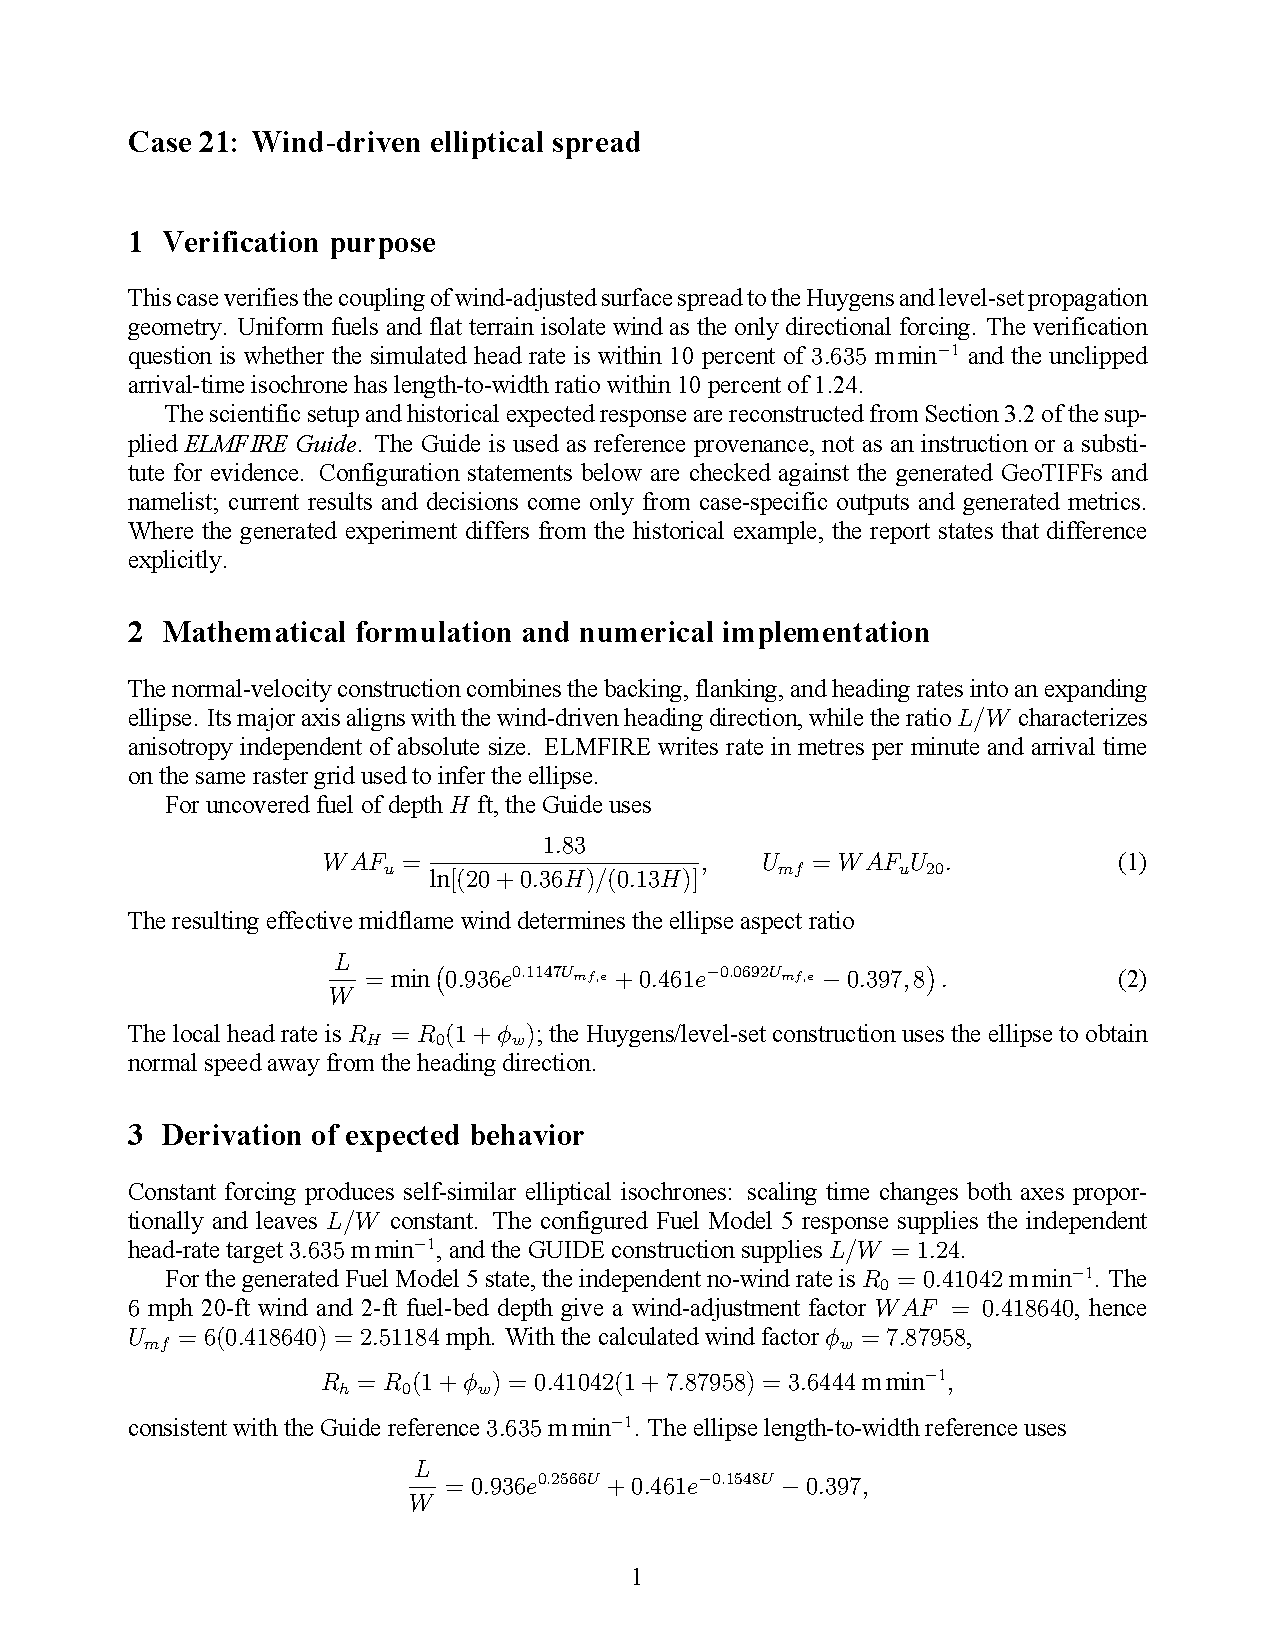
\includepdf[pages=-,pagecommand={\thispagestyle{empty}},addtotoc={1,section,1,{CASE21\_WDE -- Case 21: Wind-driven elliptical spread},case-detail:case21-wde}]{../cases/Verification/coupling_tests/CASE21_WDE/report/case_report.pdf}%
}{%
  \phantomsection
  \label{case-detail:case21-wde}
  \addcontentsline{toc}{section}{CASE21\_WDE -- Case 21: Wind-driven elliptical spread}
  \section*{CASE21\_WDE -- Case 21: Wind-driven elliptical spread}
  \textbf{NOT EVALUABLE:} the detailed case description is unavailable.
}

\clearpage
\IfFileExists{../cases/Verification/coupling_tests/CASE22_VSL/report/case_report.pdf}{%
  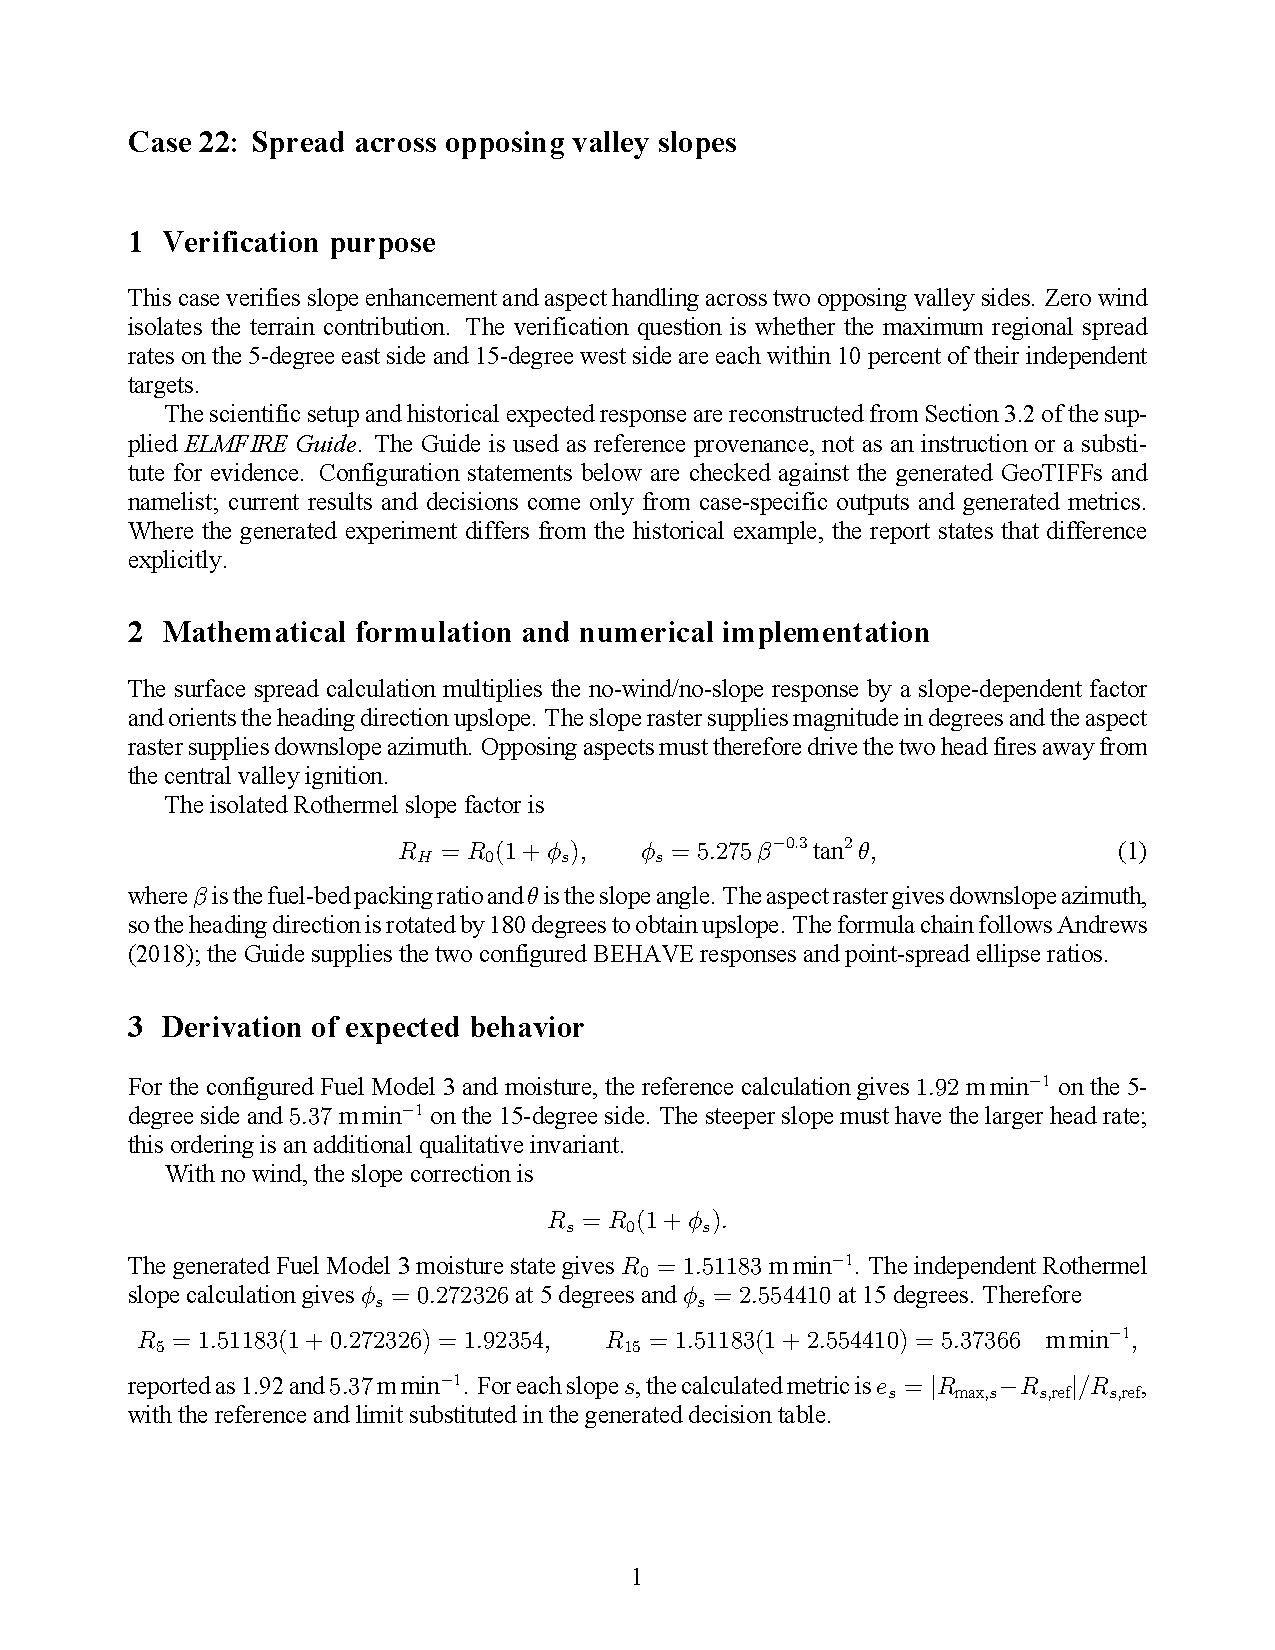
\includepdf[pages=-,pagecommand={\thispagestyle{empty}},addtotoc={1,section,1,{CASE22\_VSL -- Case 22: Spread across opposing valley slopes},case-detail:case22-vsl}]{../cases/Verification/coupling_tests/CASE22_VSL/report/case_report.pdf}%
}{%
  \phantomsection
  \label{case-detail:case22-vsl}
  \addcontentsline{toc}{section}{CASE22\_VSL -- Case 22: Spread across opposing valley slopes}
  \section*{CASE22\_VSL -- Case 22: Spread across opposing valley slopes}
  \textbf{NOT EVALUABLE:} the detailed case description is unavailable.
}

\clearpage
\IfFileExists{../cases/Verification/coupling_tests/CASE23_FQD/report/case_report.pdf}{%
  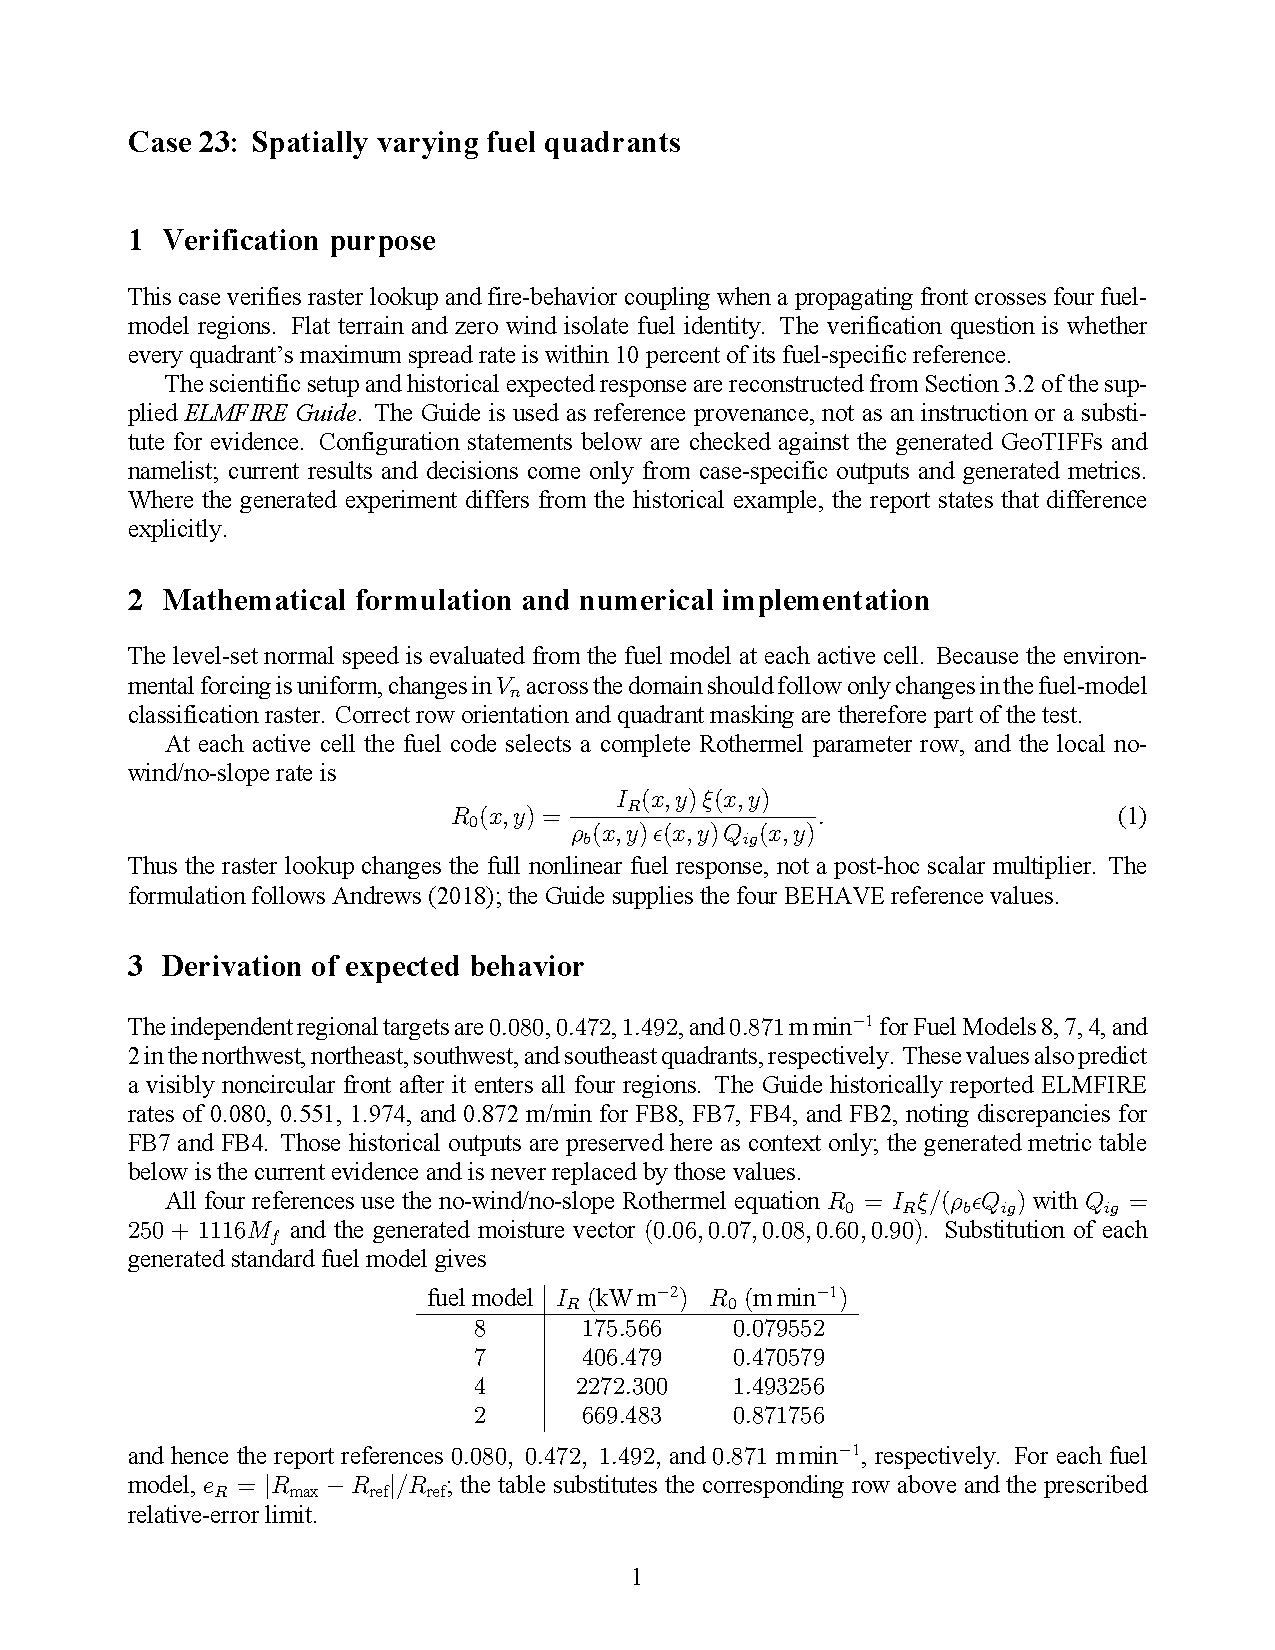
\includepdf[pages=-,pagecommand={\thispagestyle{empty}},addtotoc={1,section,1,{CASE23\_FQD -- Case 23: Spatially varying fuel quadrants},case-detail:case23-fqd}]{../cases/Verification/coupling_tests/CASE23_FQD/report/case_report.pdf}%
}{%
  \phantomsection
  \label{case-detail:case23-fqd}
  \addcontentsline{toc}{section}{CASE23\_FQD -- Case 23: Spatially varying fuel quadrants}
  \section*{CASE23\_FQD -- Case 23: Spatially varying fuel quadrants}
  \textbf{NOT EVALUABLE:} the detailed case description is unavailable.
}

\clearpage
\IfFileExists{../cases/Verification/coupling_tests/CASE24_CXI/report/case_report.pdf}{%
  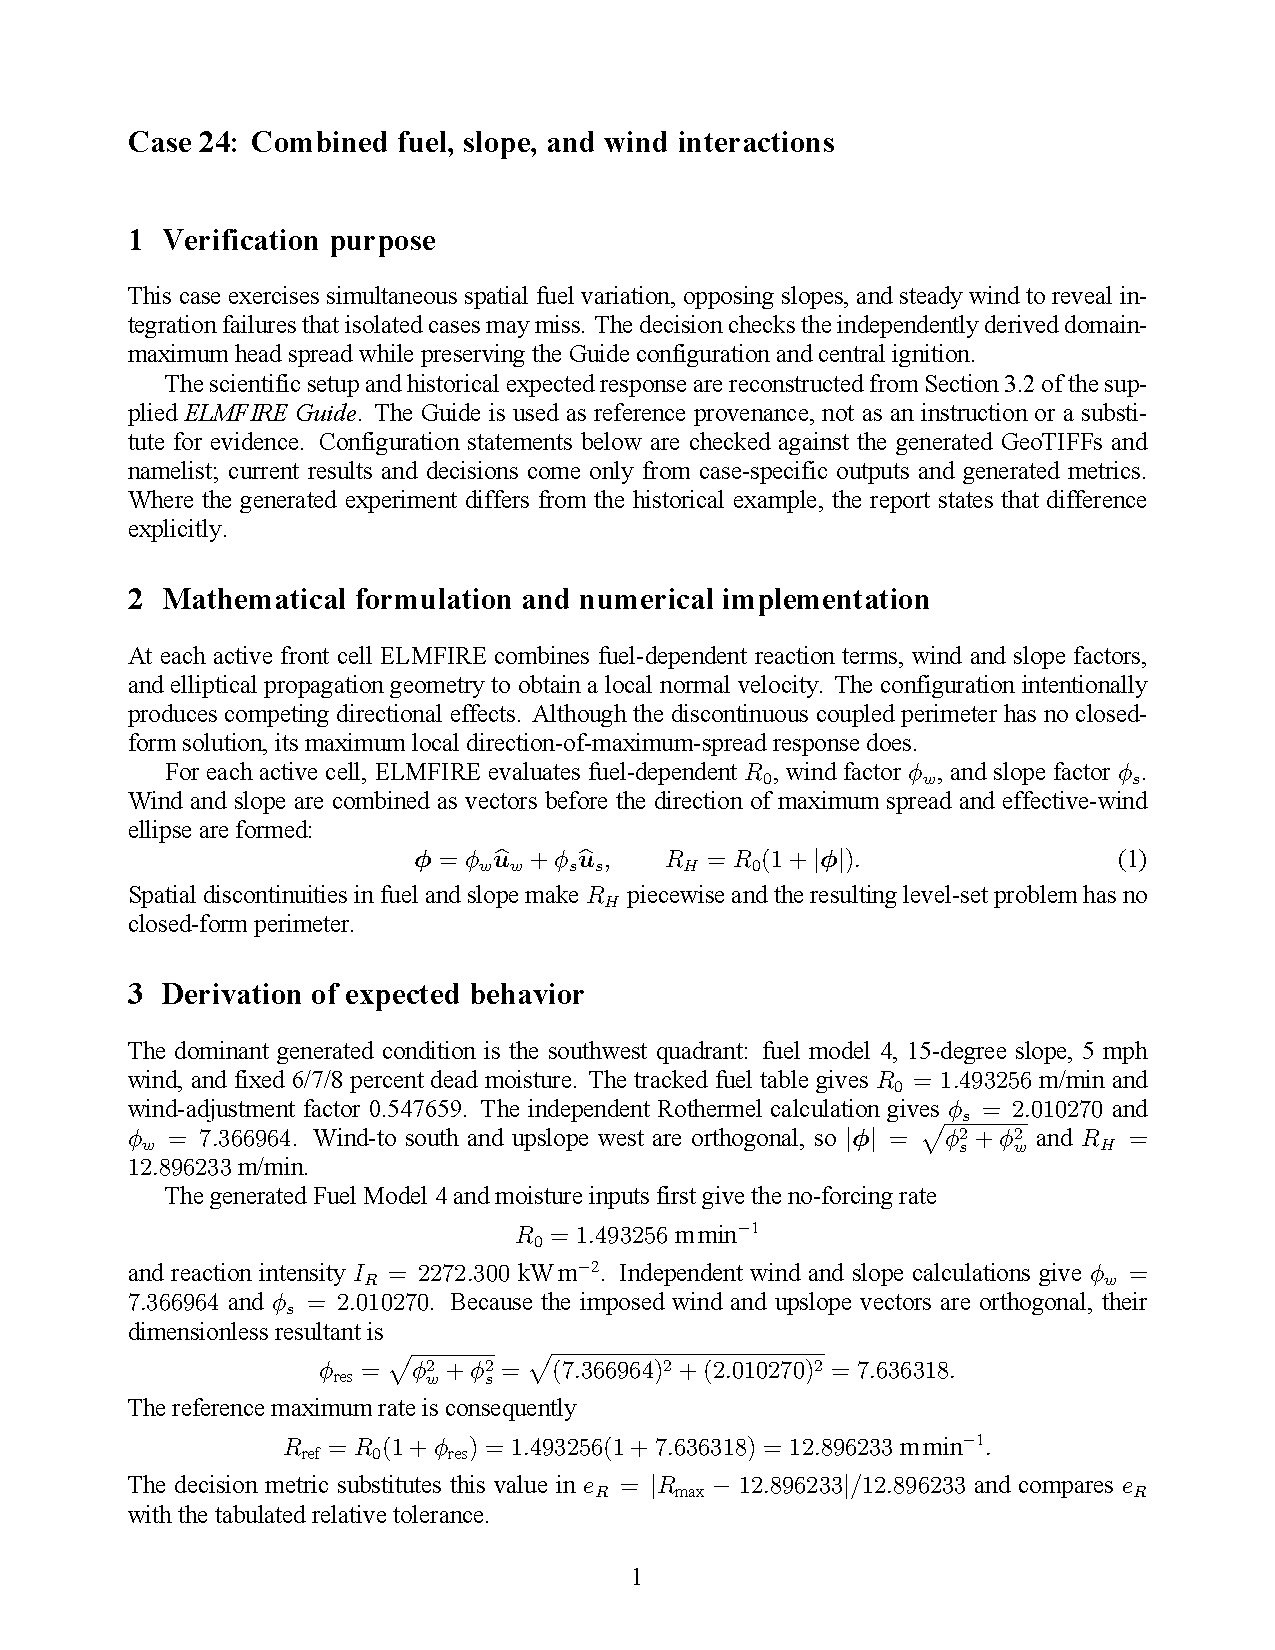
\includepdf[pages=-,pagecommand={\thispagestyle{empty}},addtotoc={1,section,1,{CASE24\_CXI -- Case 24: Combined fuel, slope, and wind interactions},case-detail:case24-cxi}]{../cases/Verification/coupling_tests/CASE24_CXI/report/case_report.pdf}%
}{%
  \phantomsection
  \label{case-detail:case24-cxi}
  \addcontentsline{toc}{section}{CASE24\_CXI -- Case 24: Combined fuel, slope, and wind interactions}
  \section*{CASE24\_CXI -- Case 24: Combined fuel, slope, and wind interactions}
  \textbf{NOT EVALUABLE:} the detailed case description is unavailable.
}

\clearpage
\IfFileExists{../cases/Verification/coupling_tests/CASE25_MQD/report/case_report.pdf}{%
  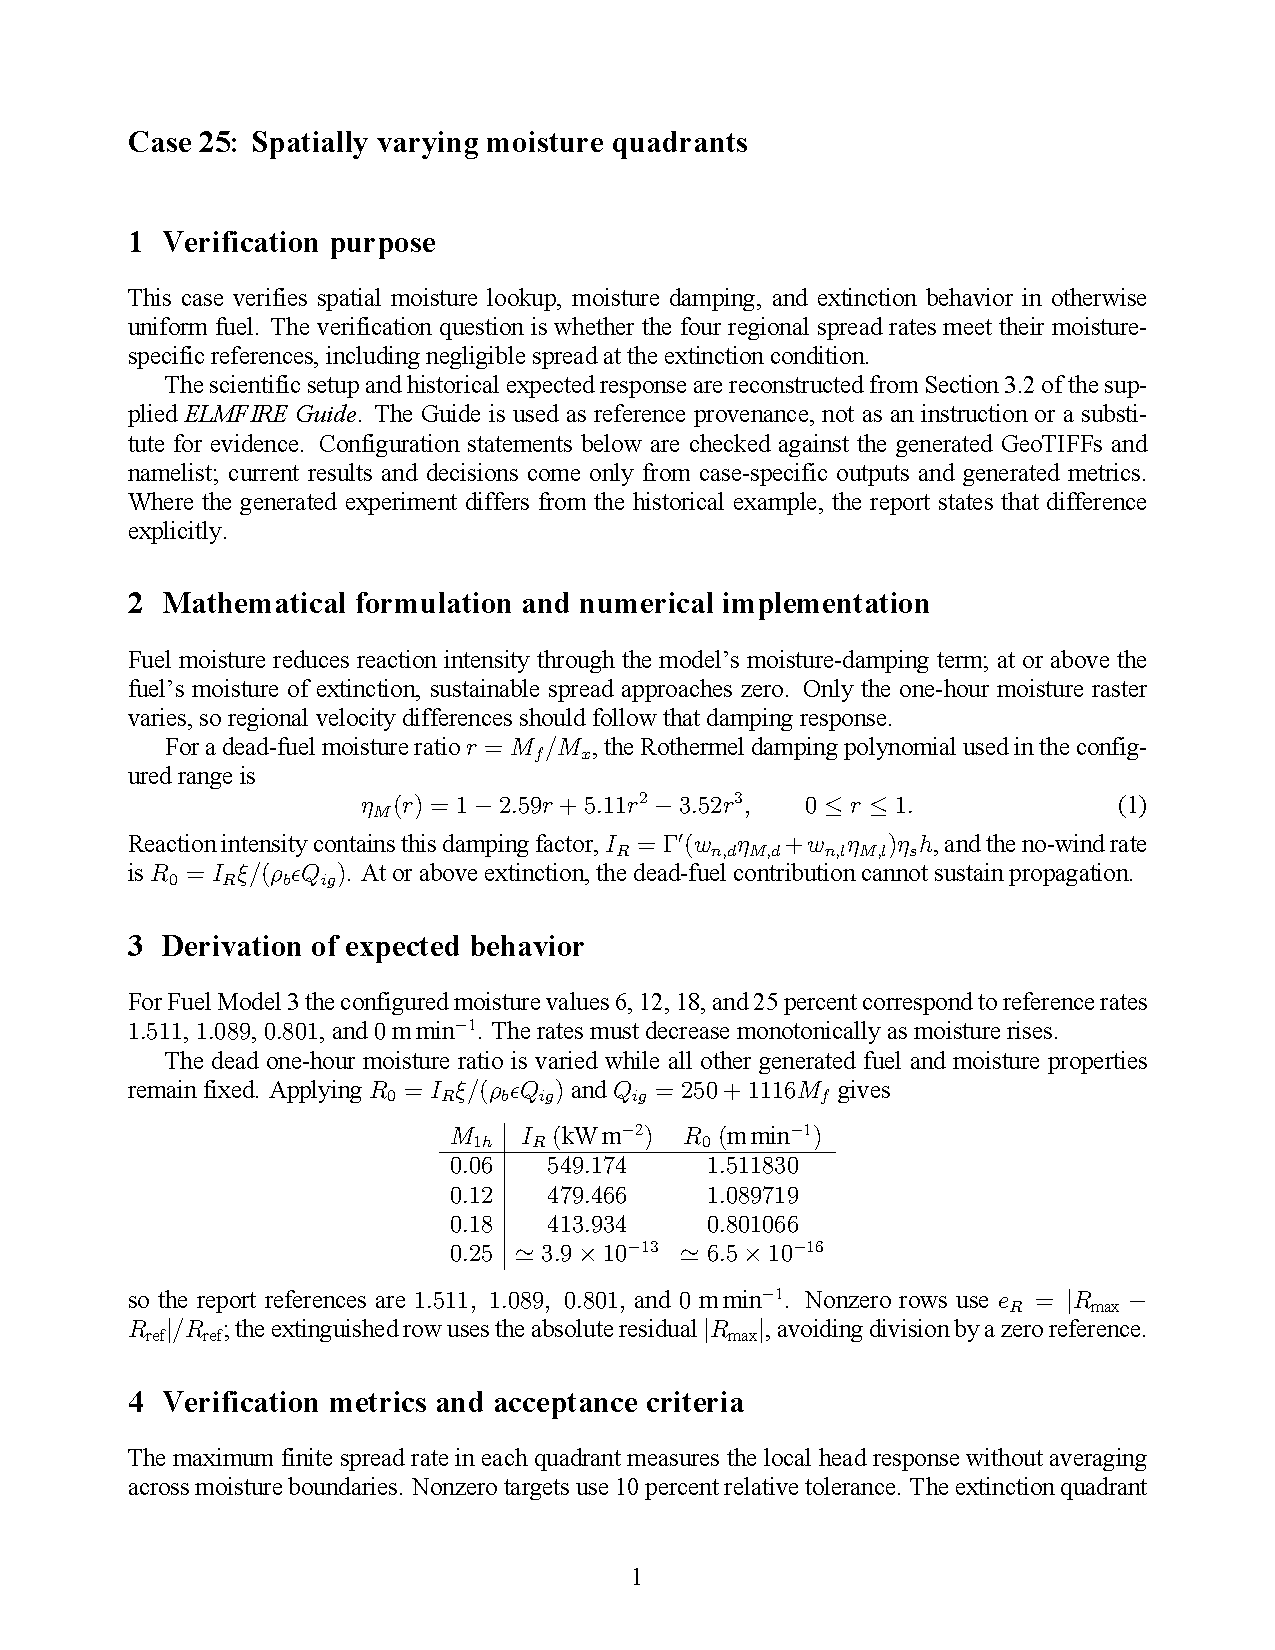
\includepdf[pages=-,pagecommand={\thispagestyle{empty}},addtotoc={1,section,1,{CASE25\_MQD -- Case 25: Spatially varying moisture quadrants},case-detail:case25-mqd}]{../cases/Verification/coupling_tests/CASE25_MQD/report/case_report.pdf}%
}{%
  \phantomsection
  \label{case-detail:case25-mqd}
  \addcontentsline{toc}{section}{CASE25\_MQD -- Case 25: Spatially varying moisture quadrants}
  \section*{CASE25\_MQD -- Case 25: Spatially varying moisture quadrants}
  \textbf{NOT EVALUABLE:} the detailed case description is unavailable.
}

\clearpage
\IfFileExists{../cases/Verification/coupling_tests/CASE26_CNF/report/case_report.pdf}{%
  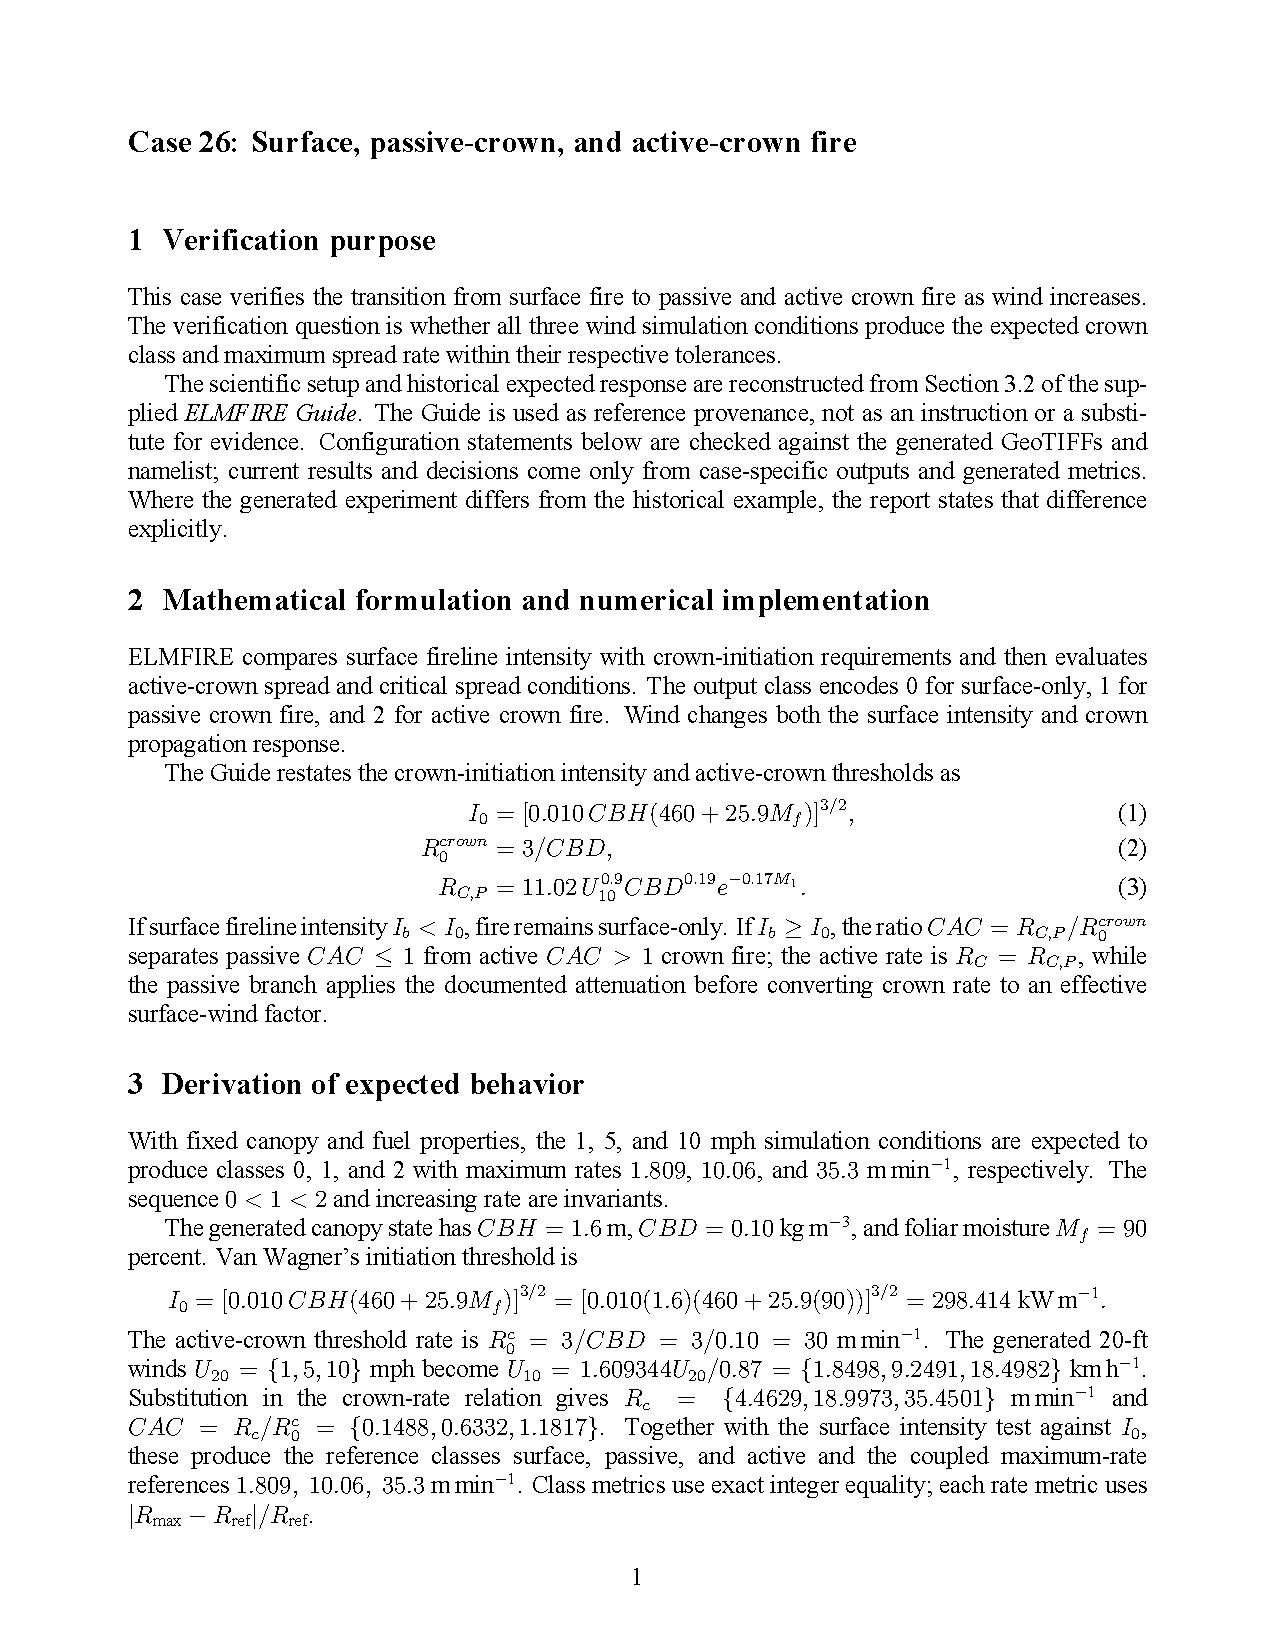
\includepdf[pages=-,pagecommand={\thispagestyle{empty}},addtotoc={1,section,1,{CASE26\_CNF -- Case 26: Surface, passive-crown, and active-crown fire},case-detail:case26-cnf}]{../cases/Verification/coupling_tests/CASE26_CNF/report/case_report.pdf}%
}{%
  \phantomsection
  \label{case-detail:case26-cnf}
  \addcontentsline{toc}{section}{CASE26\_CNF -- Case 26: Surface, passive-crown, and active-crown fire}
  \section*{CASE26\_CNF -- Case 26: Surface, passive-crown, and active-crown fire}
  \textbf{NOT EVALUABLE:} the detailed case description is unavailable.
}

\clearpage
\IfFileExists{../cases/Verification/coupling_tests/CASE27_FBT/report/case_report.pdf}{%
  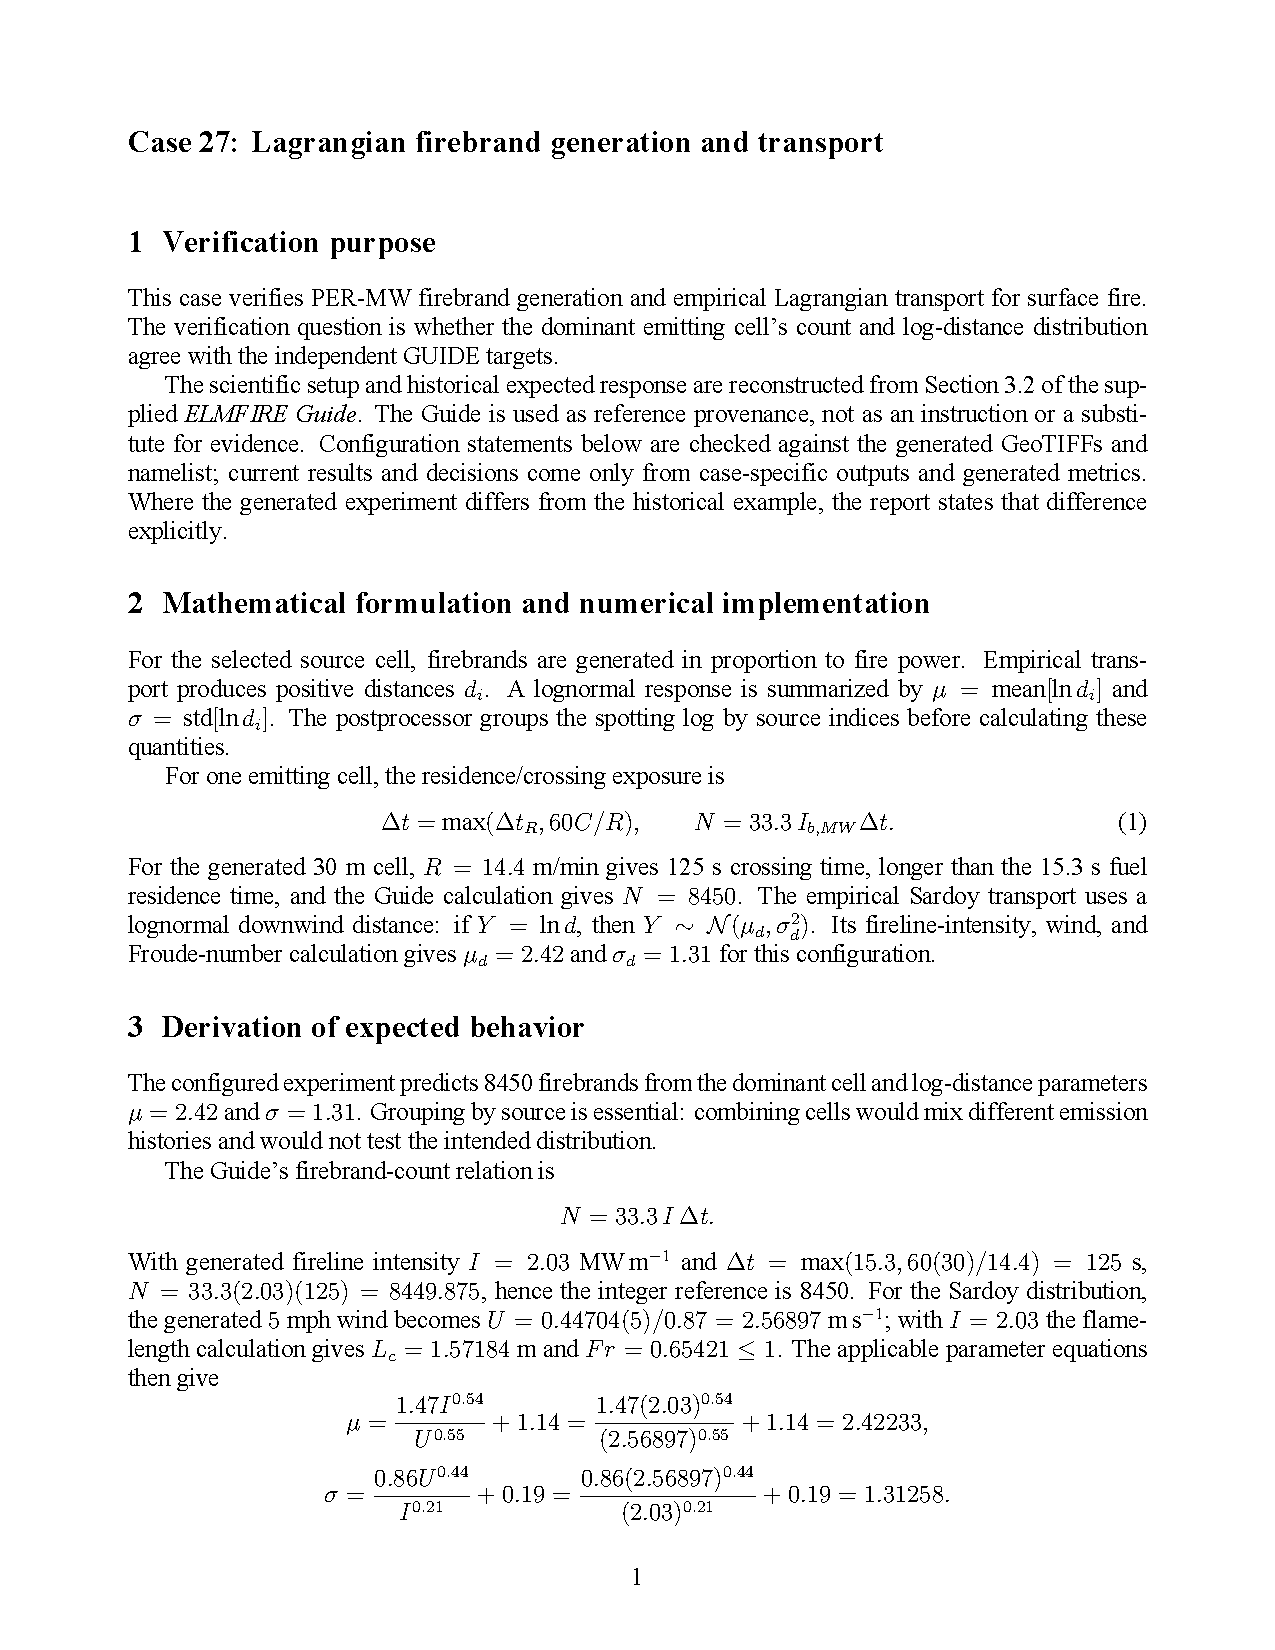
\includepdf[pages=-,pagecommand={\thispagestyle{empty}},addtotoc={1,section,1,{CASE27\_FBT -- Case 27: Lagrangian firebrand generation and transport},case-detail:case27-fbt}]{../cases/Verification/coupling_tests/CASE27_FBT/report/case_report.pdf}%
}{%
  \phantomsection
  \label{case-detail:case27-fbt}
  \addcontentsline{toc}{section}{CASE27\_FBT -- Case 27: Lagrangian firebrand generation and transport}
  \section*{CASE27\_FBT -- Case 27: Lagrangian firebrand generation and transport}
  \textbf{NOT EVALUABLE:} the detailed case description is unavailable.
}

\clearpage
\IfFileExists{../cases/Verification/coupling_tests/CASE28_OVA/report/case_report.pdf}{%
  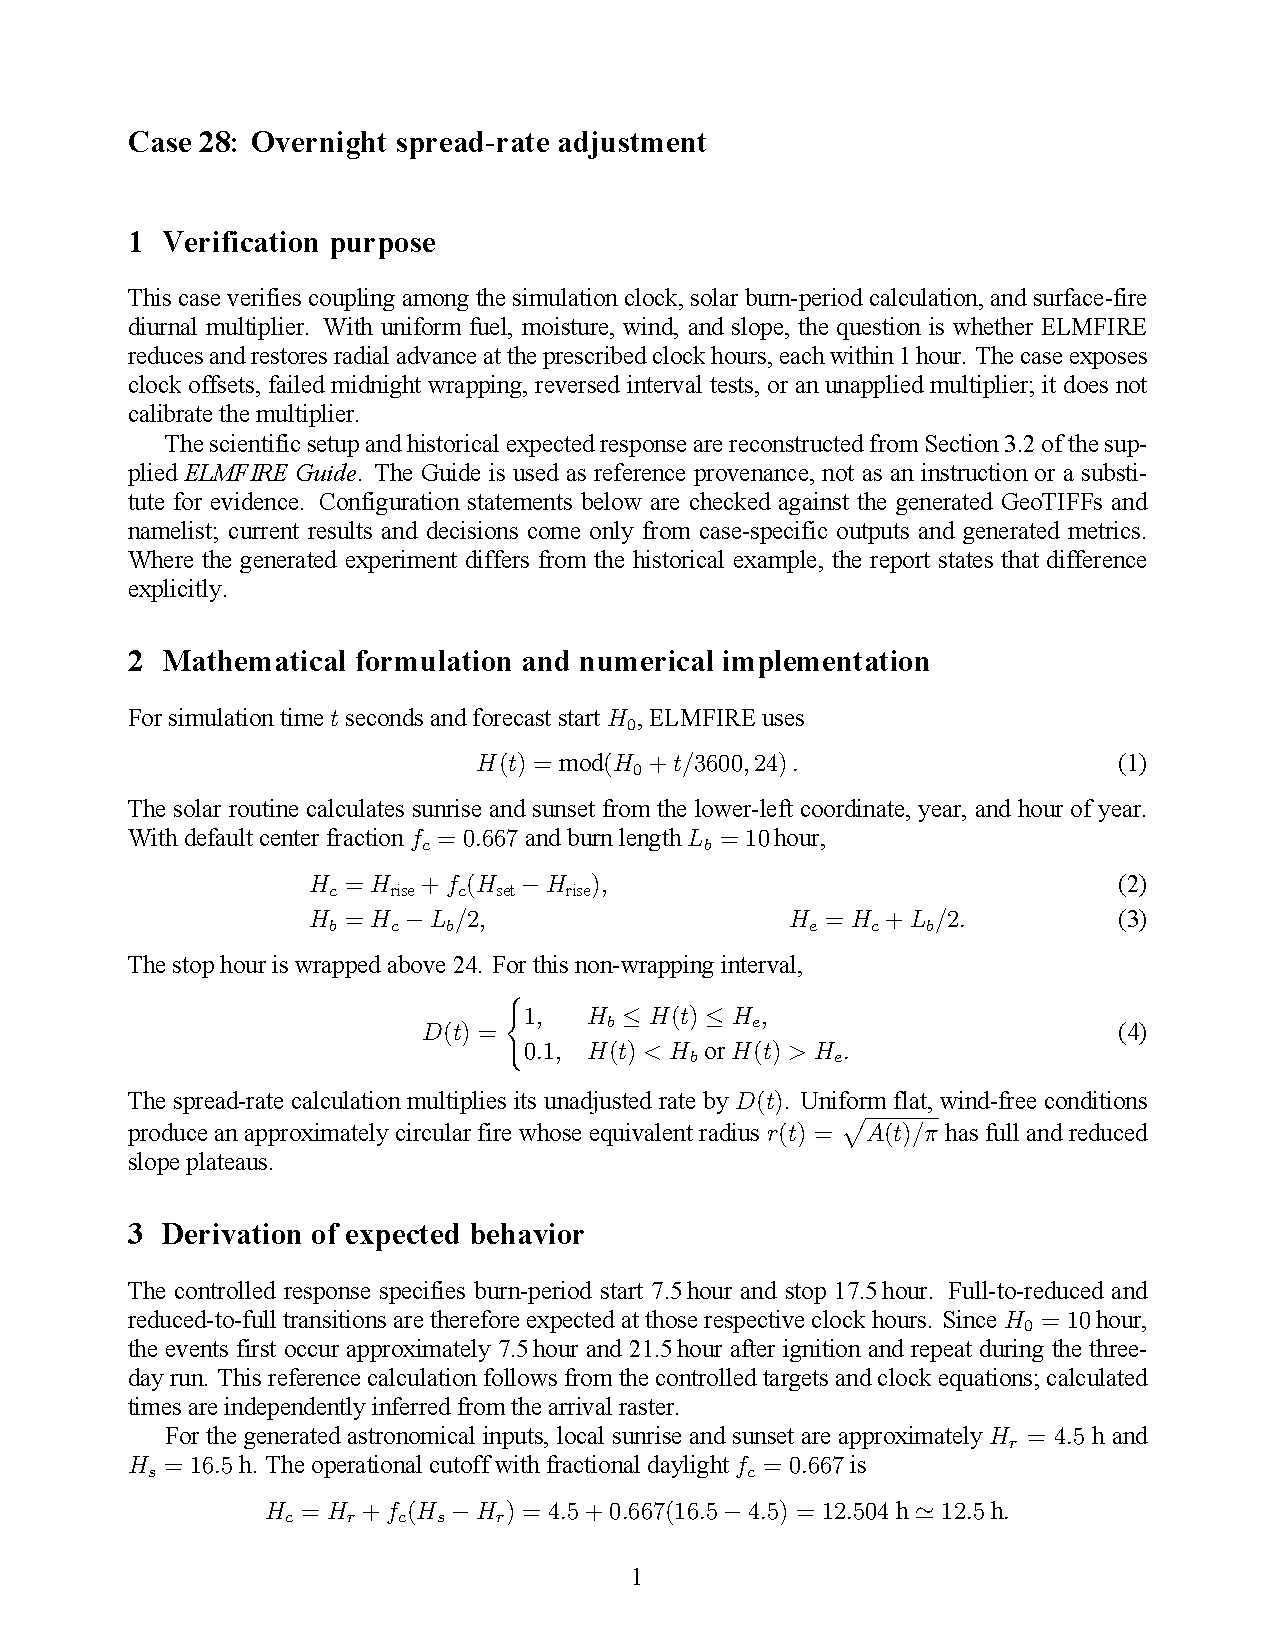
\includepdf[pages=-,pagecommand={\thispagestyle{empty}},addtotoc={1,section,1,{CASE28\_OVA -- Case 28: Overnight spread-rate adjustment},case-detail:case28-ova}]{../cases/Verification/coupling_tests/CASE28_OVA/report/case_report.pdf}%
}{%
  \phantomsection
  \label{case-detail:case28-ova}
  \addcontentsline{toc}{section}{CASE28\_OVA -- Case 28: Overnight spread-rate adjustment}
  \section*{CASE28\_OVA -- Case 28: Overnight spread-rate adjustment}
  \textbf{NOT EVALUABLE:} the detailed case description is unavailable.
}

\clearpage
\IfFileExists{../cases/Verification/coupling_tests/CASE29_SUP/report/case_report.pdf}{%
  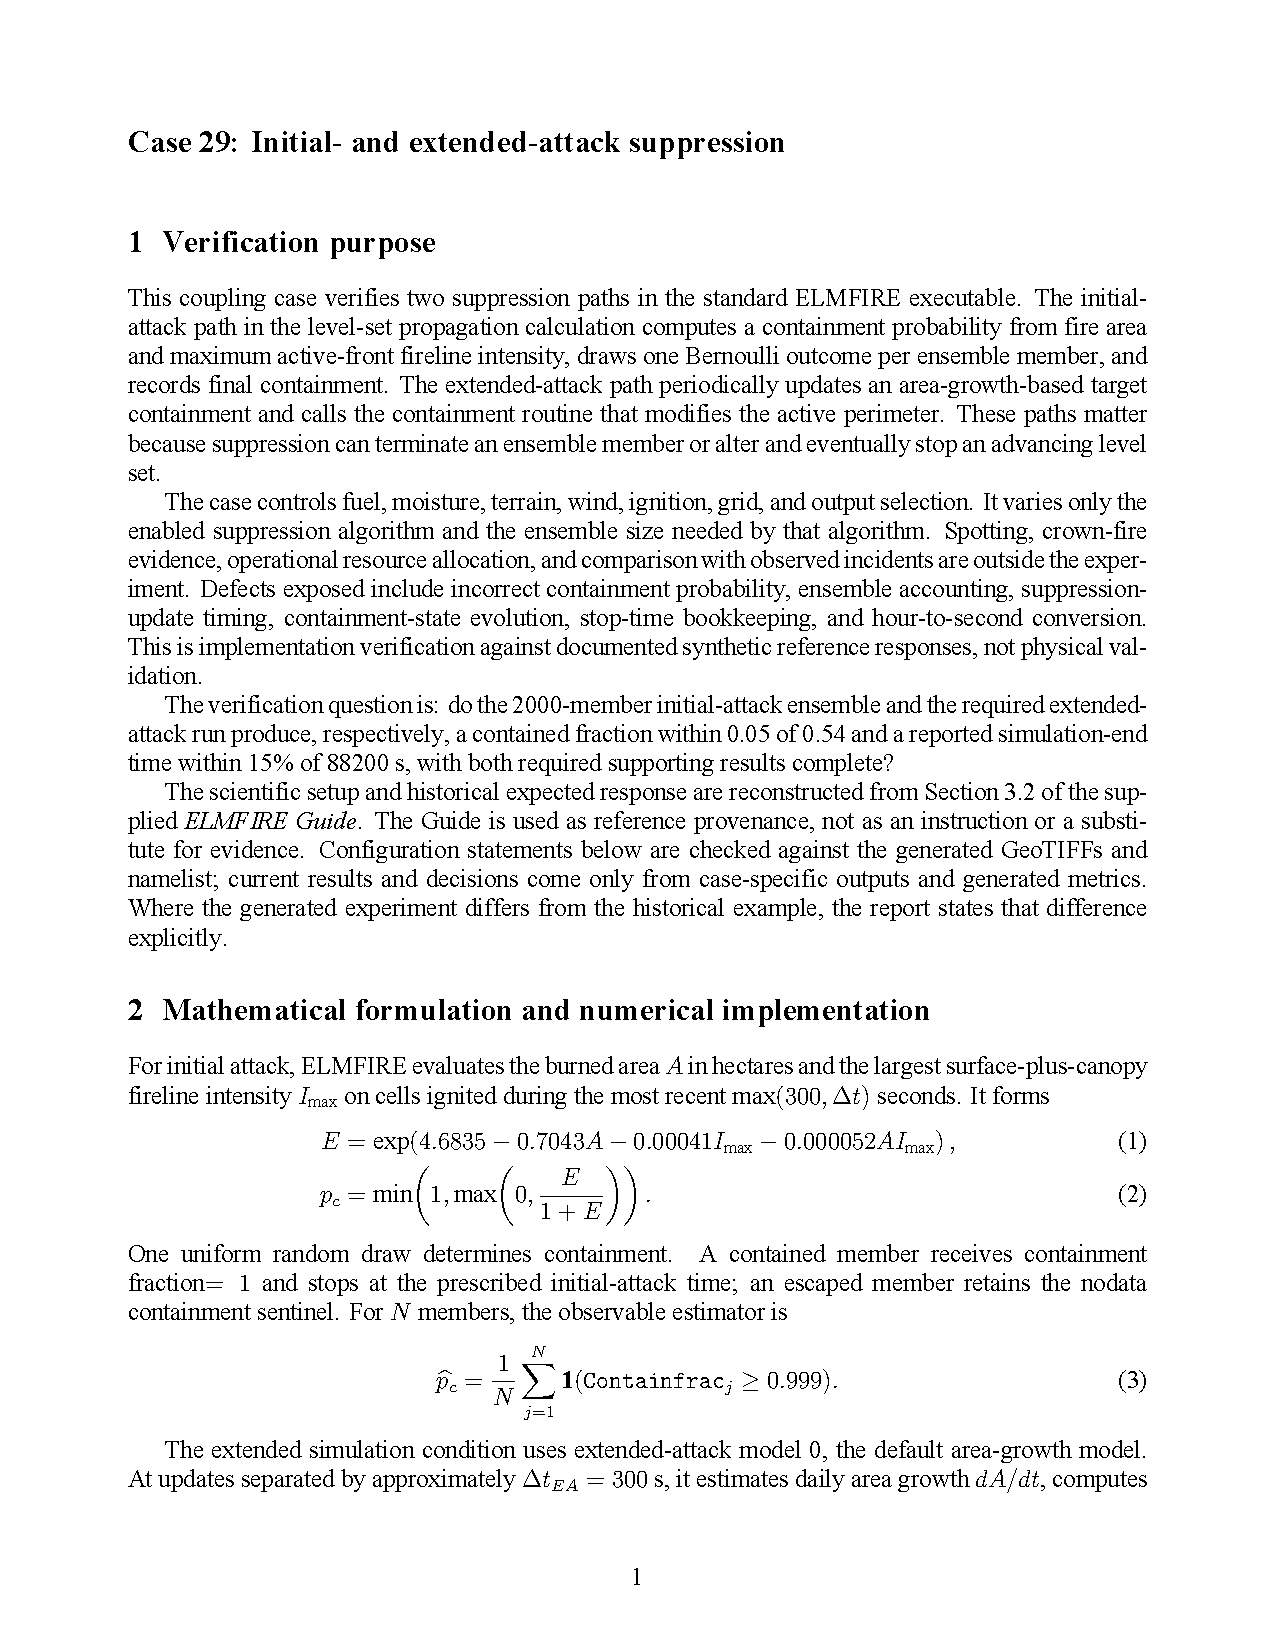
\includepdf[pages=-,pagecommand={\thispagestyle{empty}},addtotoc={1,section,1,{CASE29\_SUP -- Case 29: Initial- and extended-attack suppression},case-detail:case29-sup}]{../cases/Verification/coupling_tests/CASE29_SUP/report/case_report.pdf}%
}{%
  \phantomsection
  \label{case-detail:case29-sup}
  \addcontentsline{toc}{section}{CASE29\_SUP -- Case 29: Initial- and extended-attack suppression}
  \section*{CASE29\_SUP -- Case 29: Initial- and extended-attack suppression}
  \textbf{NOT EVALUABLE:} the detailed case description is unavailable.
}

\clearpage
\IfFileExists{../cases/Verification/coupling_tests/CASE30_MIT/report/case_report.pdf}{%
  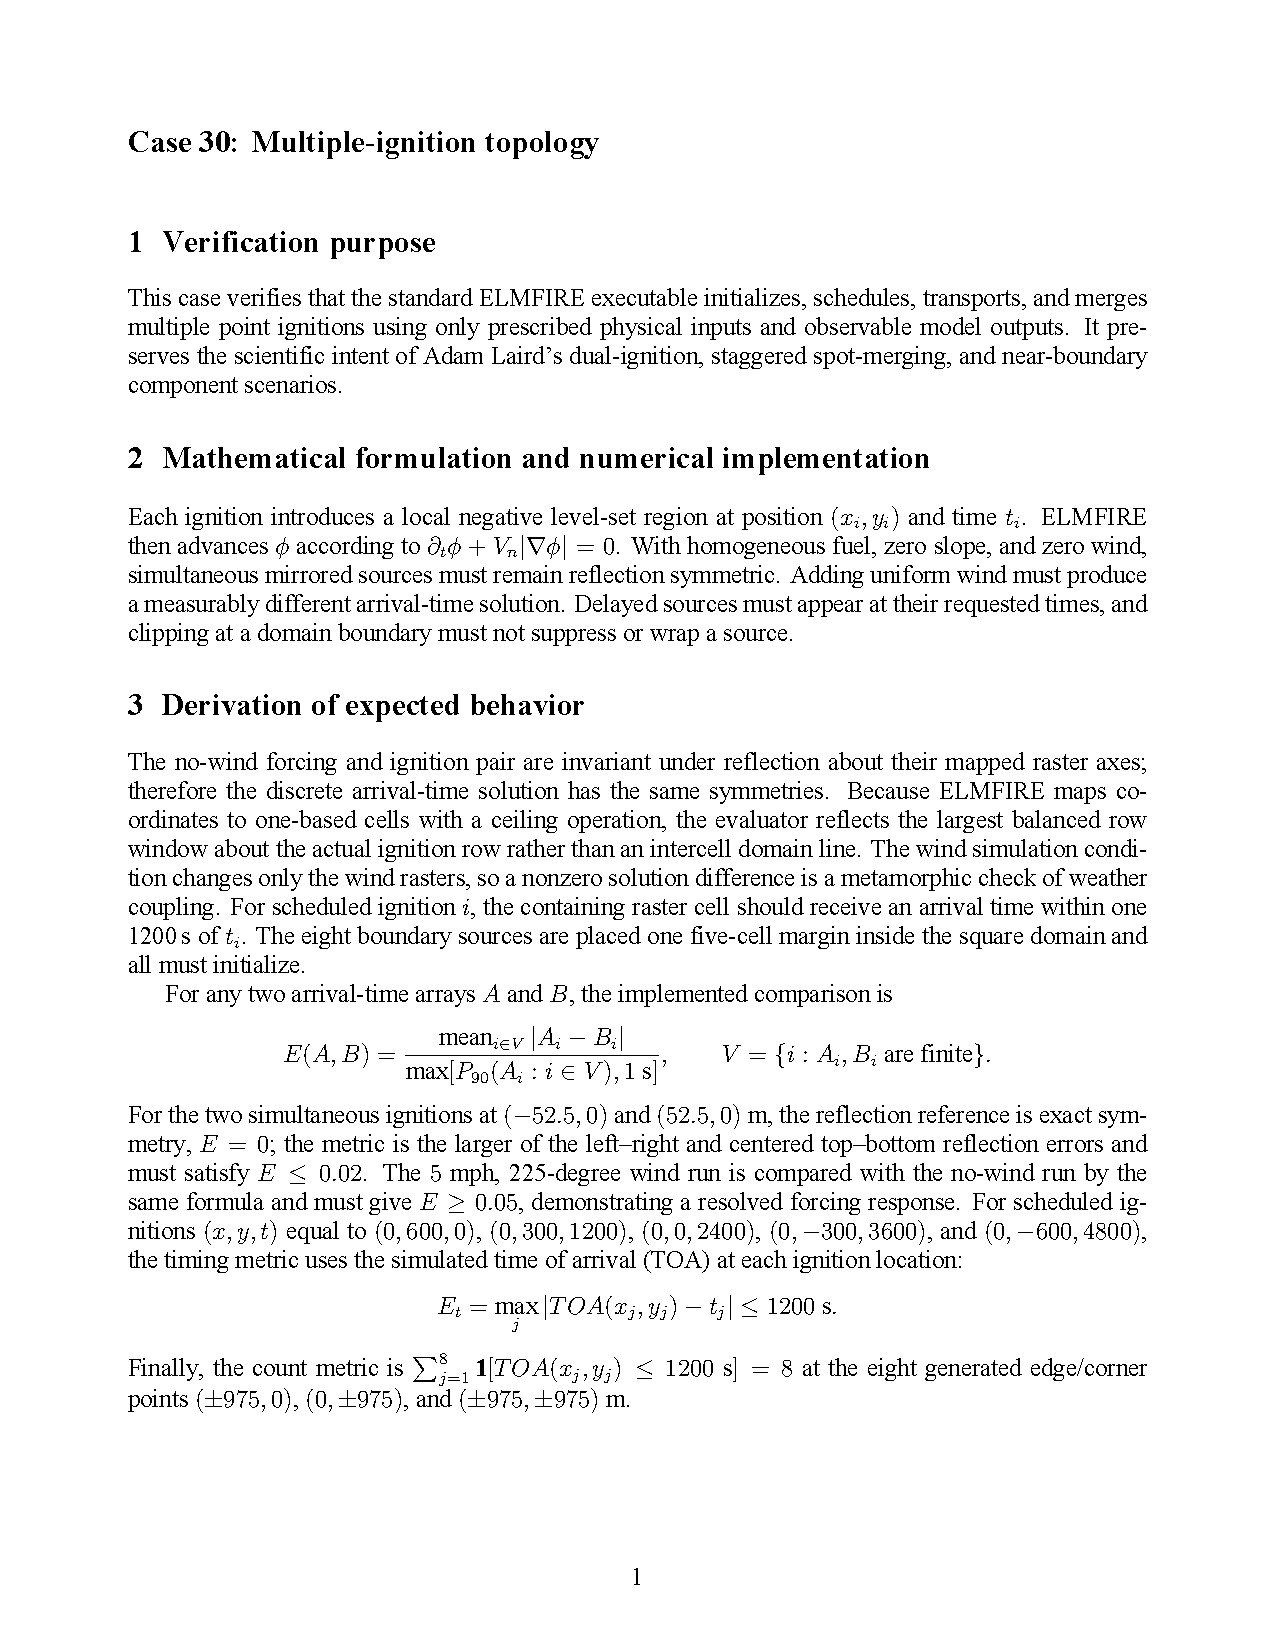
\includepdf[pages=-,pagecommand={\thispagestyle{empty}},addtotoc={1,section,1,{CASE30\_MIT -- Case 30: Multiple-ignition topology},case-detail:case30-mit}]{../cases/Verification/coupling_tests/CASE30_MIT/report/case_report.pdf}%
}{%
  \phantomsection
  \label{case-detail:case30-mit}
  \addcontentsline{toc}{section}{CASE30\_MIT -- Case 30: Multiple-ignition topology}
  \section*{CASE30\_MIT -- Case 30: Multiple-ignition topology}
  \textbf{NOT EVALUABLE:} the detailed case description is unavailable.
}

\clearpage
\IfFileExists{../cases/Verification/coupling_tests/CASE31_PFT/report/case_report.pdf}{%
  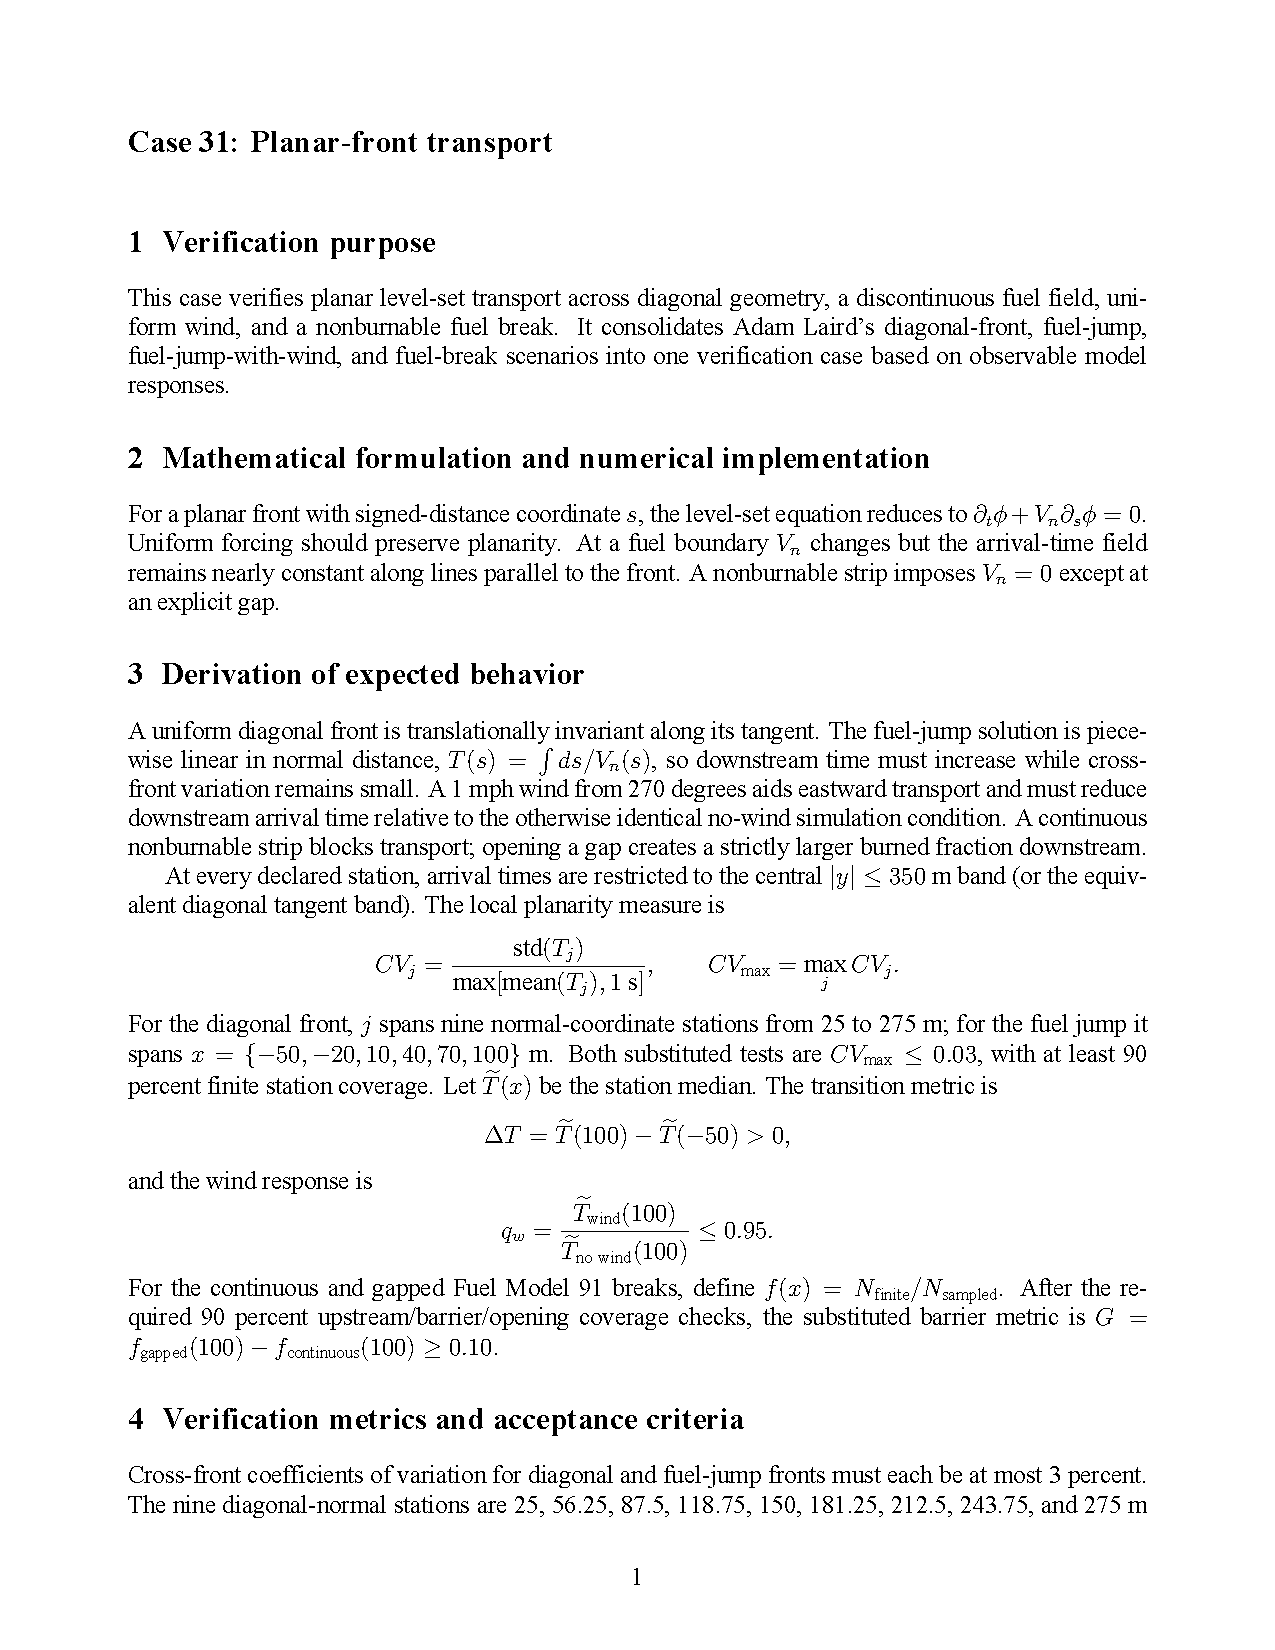
\includepdf[pages=-,pagecommand={\thispagestyle{empty}},addtotoc={1,section,1,{CASE31\_PFT -- Case 31: Planar-front transport},case-detail:case31-pft}]{../cases/Verification/coupling_tests/CASE31_PFT/report/case_report.pdf}%
}{%
  \phantomsection
  \label{case-detail:case31-pft}
  \addcontentsline{toc}{section}{CASE31\_PFT -- Case 31: Planar-front transport}
  \section*{CASE31\_PFT -- Case 31: Planar-front transport}
  \textbf{NOT EVALUABLE:} the detailed case description is unavailable.
}

\clearpage
\IfFileExists{../cases/Verification/coupling_tests/CASE32_RCV/report/case_report.pdf}{%
  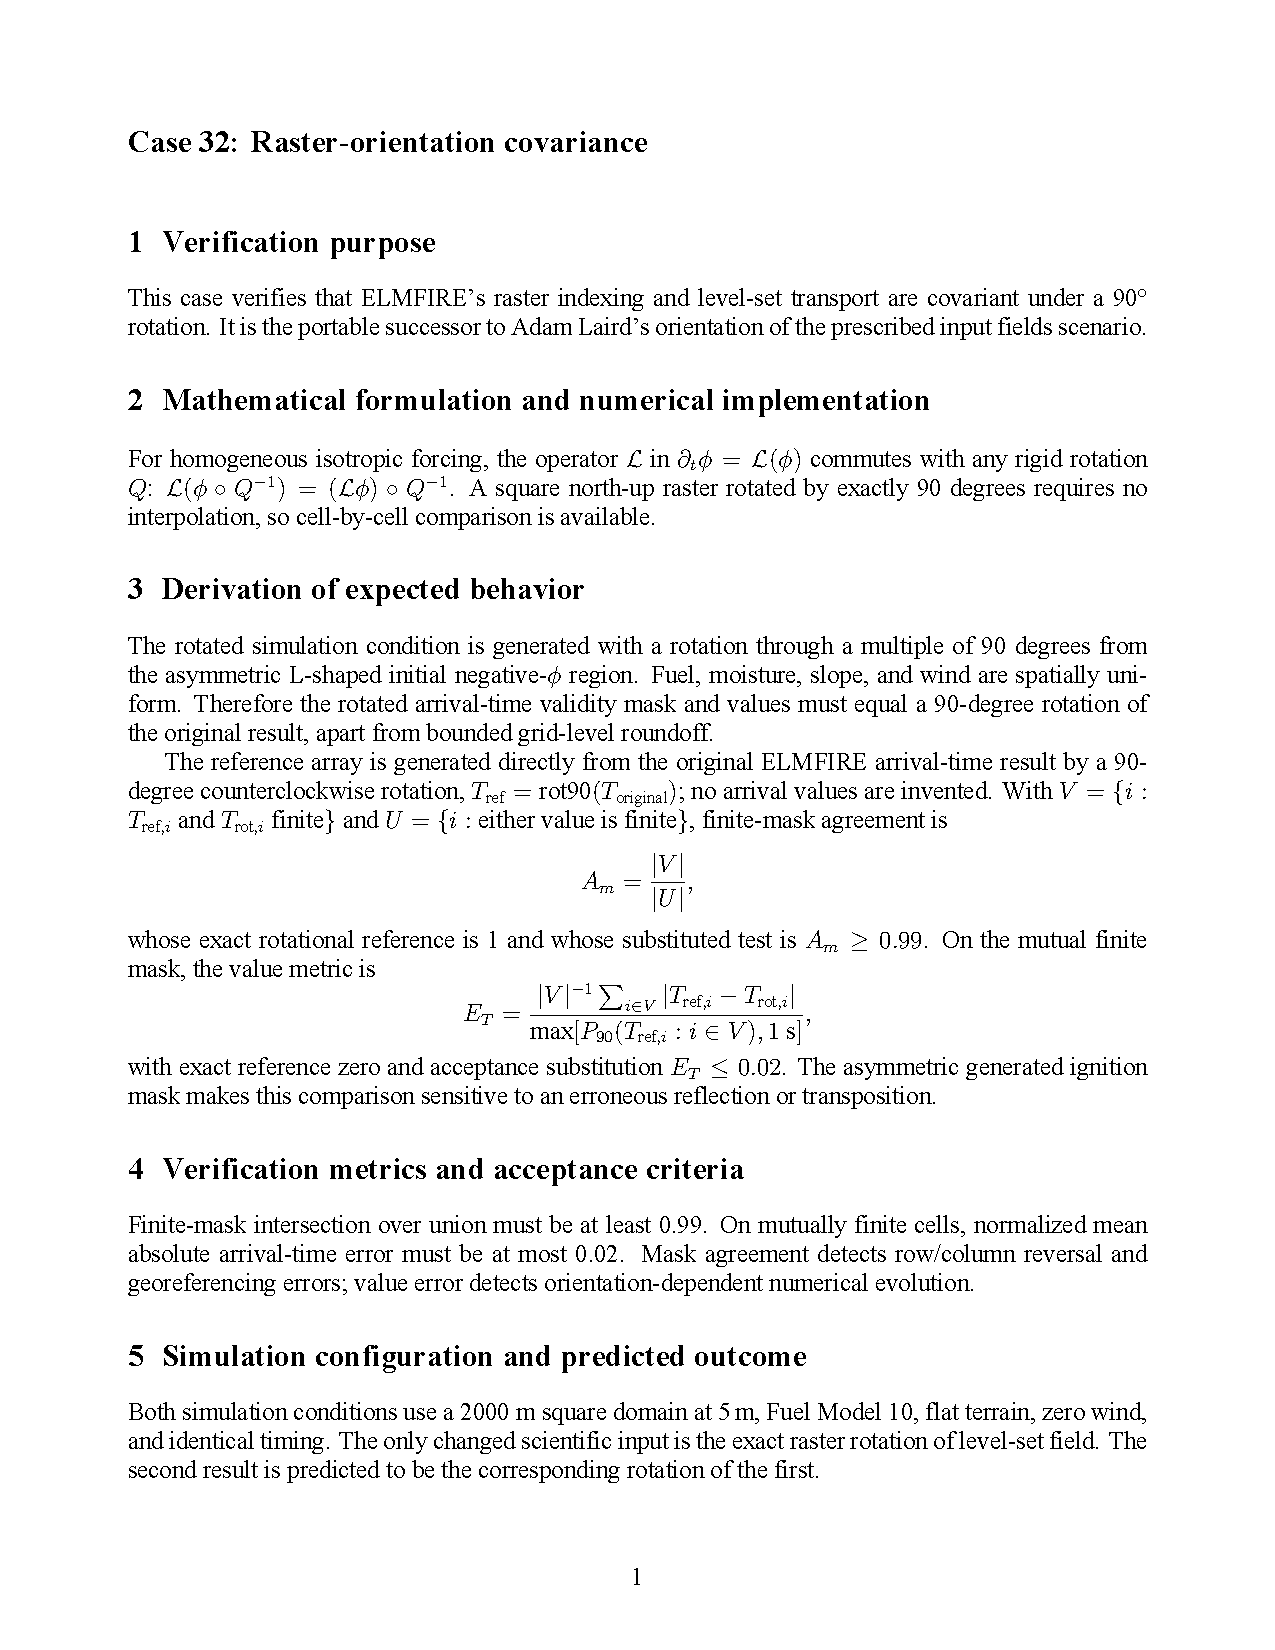
\includepdf[pages=-,pagecommand={\thispagestyle{empty}},addtotoc={1,section,1,{CASE32\_RCV -- Case 32: Raster-orientation covariance},case-detail:case32-rcv}]{../cases/Verification/coupling_tests/CASE32_RCV/report/case_report.pdf}%
}{%
  \phantomsection
  \label{case-detail:case32-rcv}
  \addcontentsline{toc}{section}{CASE32\_RCV -- Case 32: Raster-orientation covariance}
  \section*{CASE32\_RCV -- Case 32: Raster-orientation covariance}
  \textbf{NOT EVALUABLE:} the detailed case description is unavailable.
}

\clearpage
\IfFileExists{../cases/Verification/coupling_tests/CASE33_SDO/report/case_report.pdf}{%
  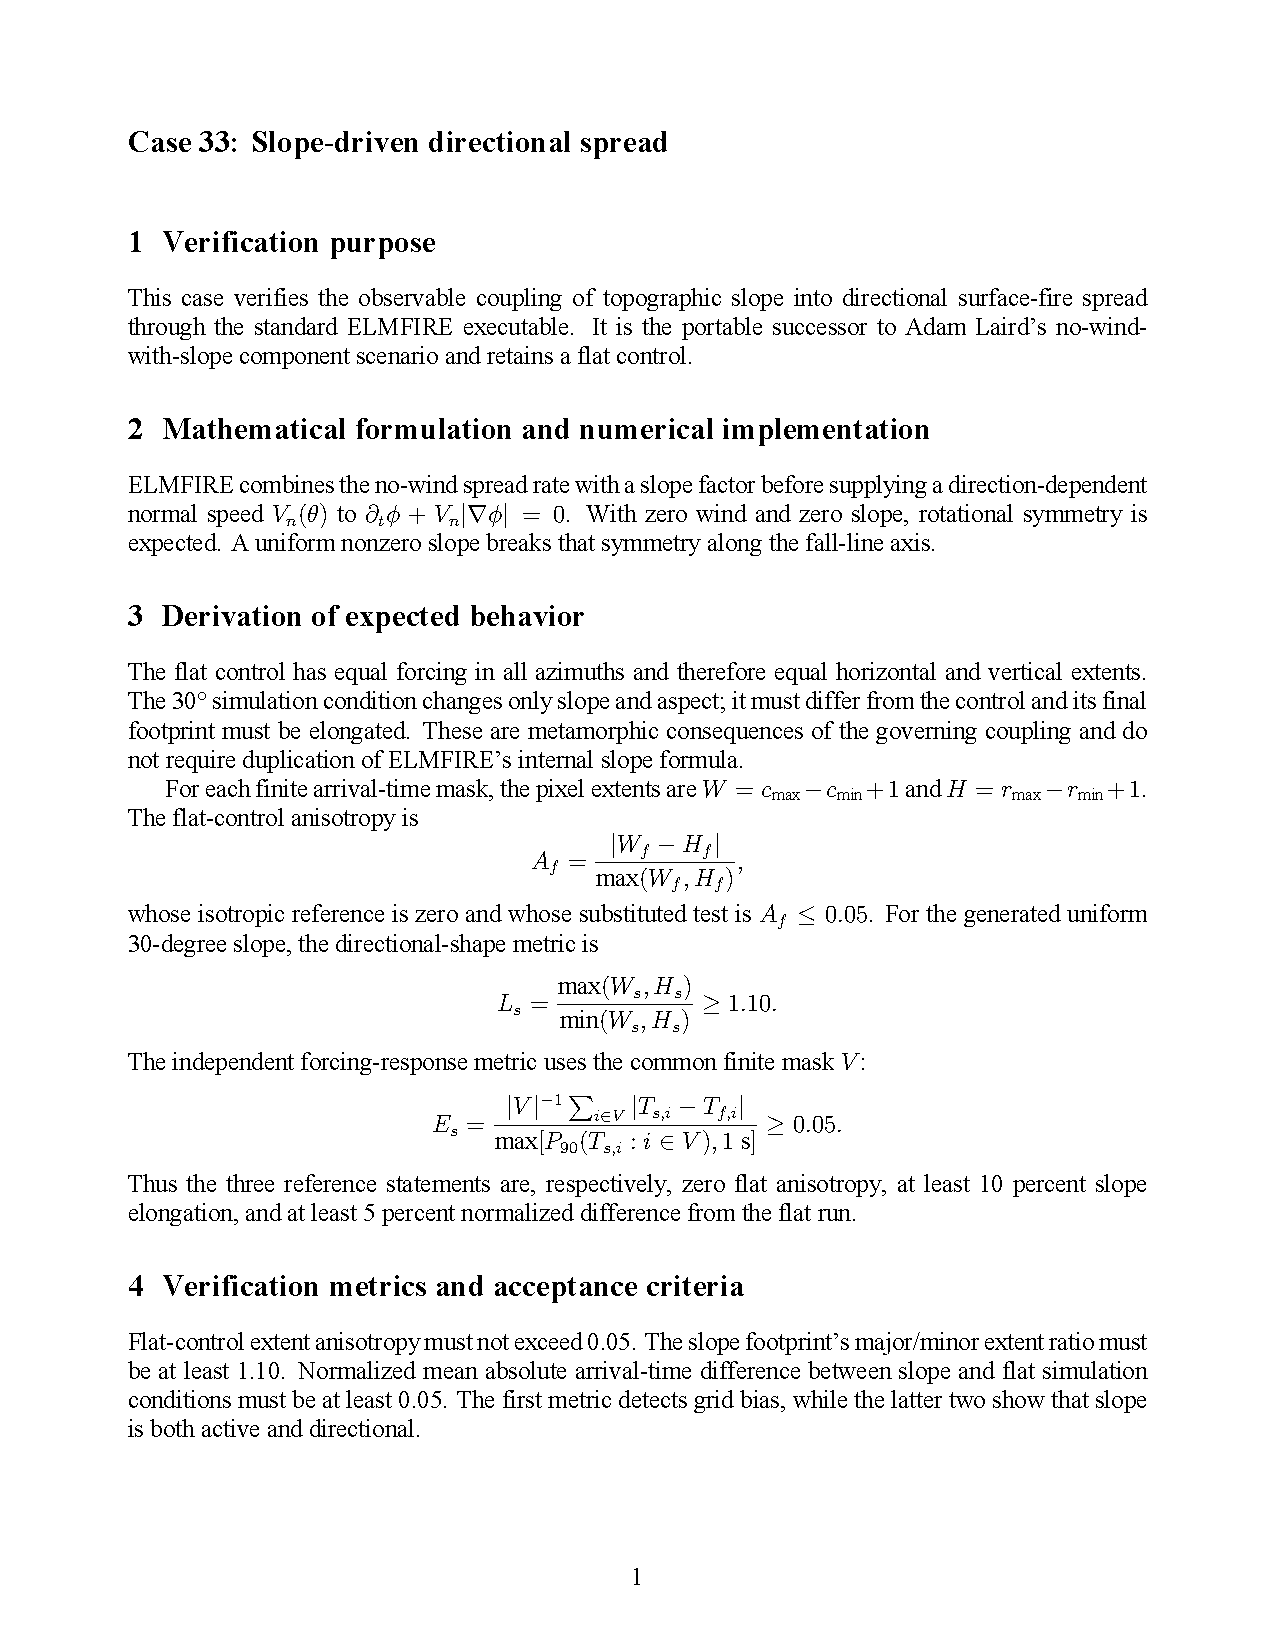
\includepdf[pages=-,pagecommand={\thispagestyle{empty}},addtotoc={1,section,1,{CASE33\_SDO -- Case 33: Slope-driven directional spread},case-detail:case33-sdo}]{../cases/Verification/coupling_tests/CASE33_SDO/report/case_report.pdf}%
}{%
  \phantomsection
  \label{case-detail:case33-sdo}
  \addcontentsline{toc}{section}{CASE33\_SDO -- Case 33: Slope-driven directional spread}
  \section*{CASE33\_SDO -- Case 33: Slope-driven directional spread}
  \textbf{NOT EVALUABLE:} the detailed case description is unavailable.
}

\clearpage
\IfFileExists{../cases/Verification/unit_tests/CASE34_FMS/report/case_report.pdf}{%
  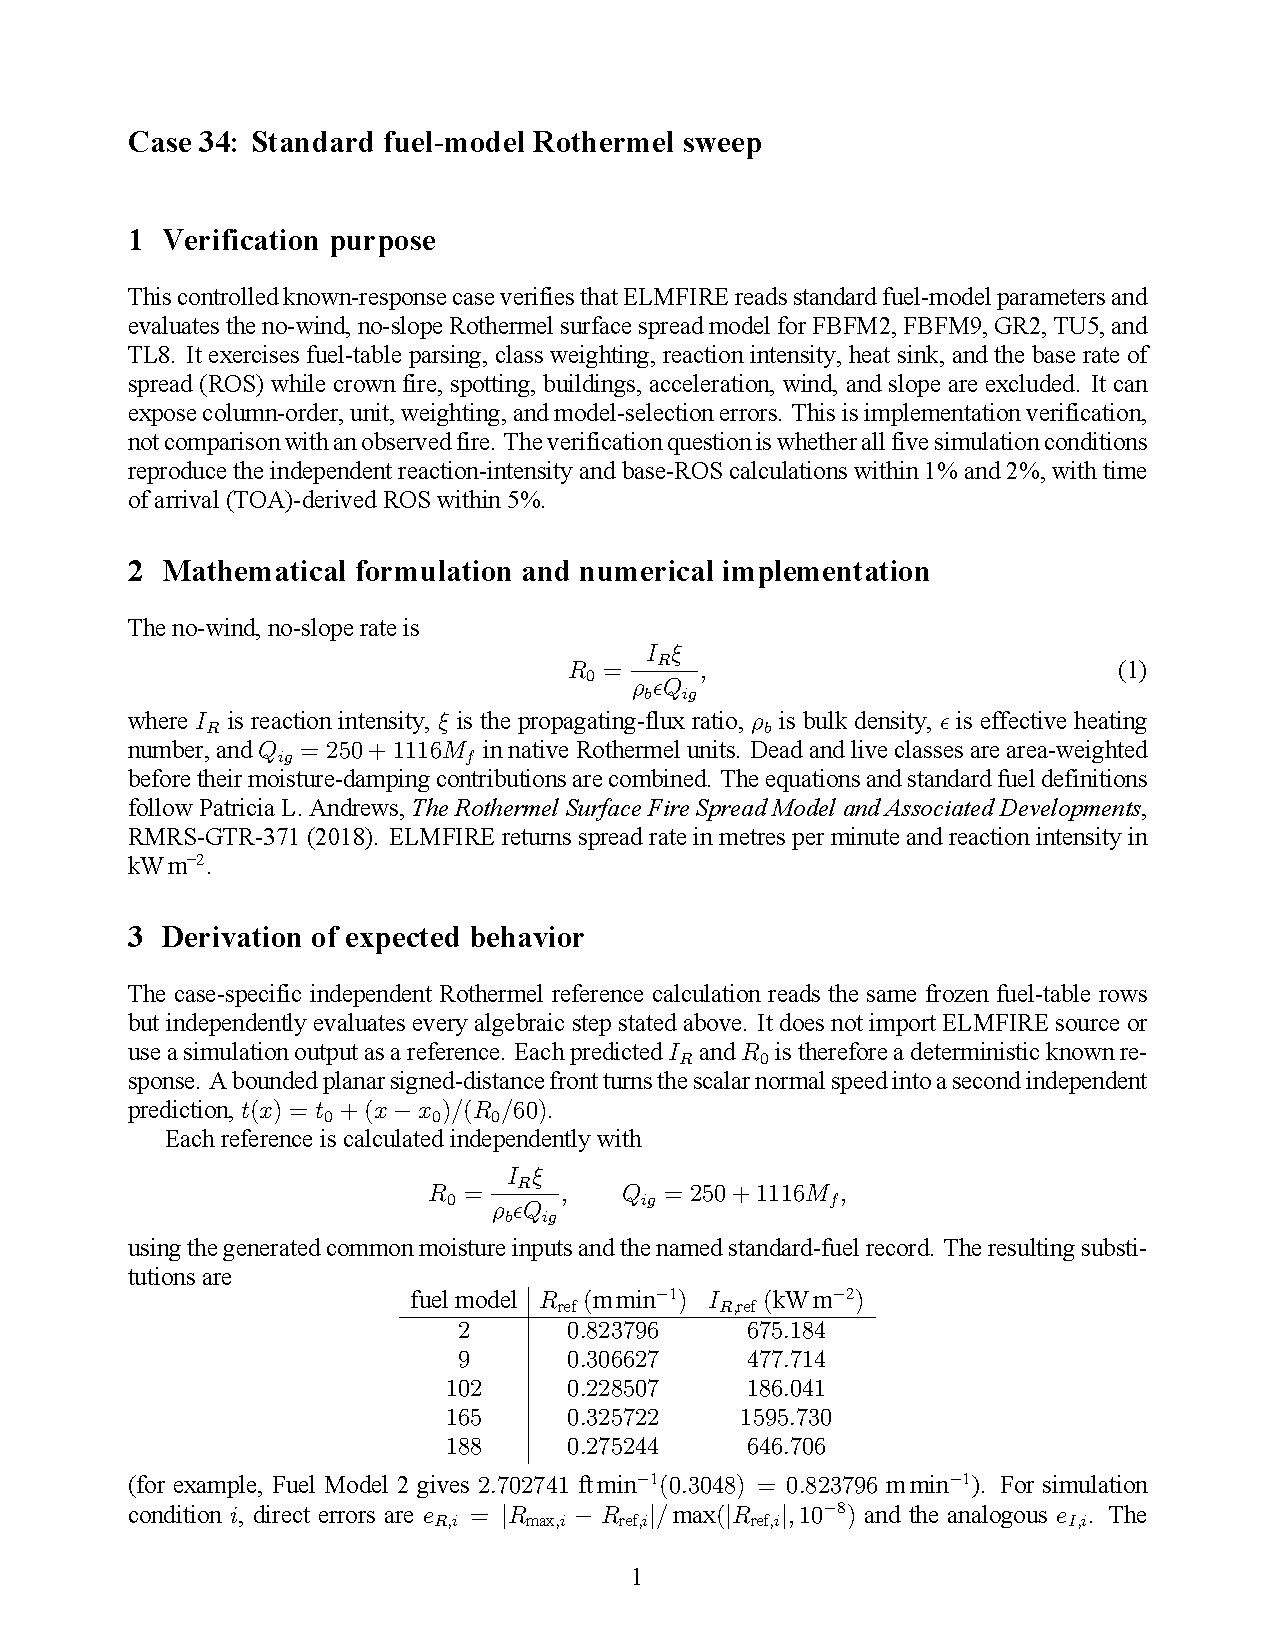
\includepdf[pages=-,pagecommand={\thispagestyle{empty}},addtotoc={1,section,1,{CASE34\_FMS -- Case 34: Standard fuel-model Rothermel sweep},case-detail:case34-fms}]{../cases/Verification/unit_tests/CASE34_FMS/report/case_report.pdf}%
}{%
  \phantomsection
  \label{case-detail:case34-fms}
  \addcontentsline{toc}{section}{CASE34\_FMS -- Case 34: Standard fuel-model Rothermel sweep}
  \section*{CASE34\_FMS -- Case 34: Standard fuel-model Rothermel sweep}
  \textbf{NOT EVALUABLE:} the detailed case description is unavailable.
}

\clearpage
\IfFileExists{../cases/Verification/unit_tests/CASE35_WSS/report/case_report.pdf}{%
  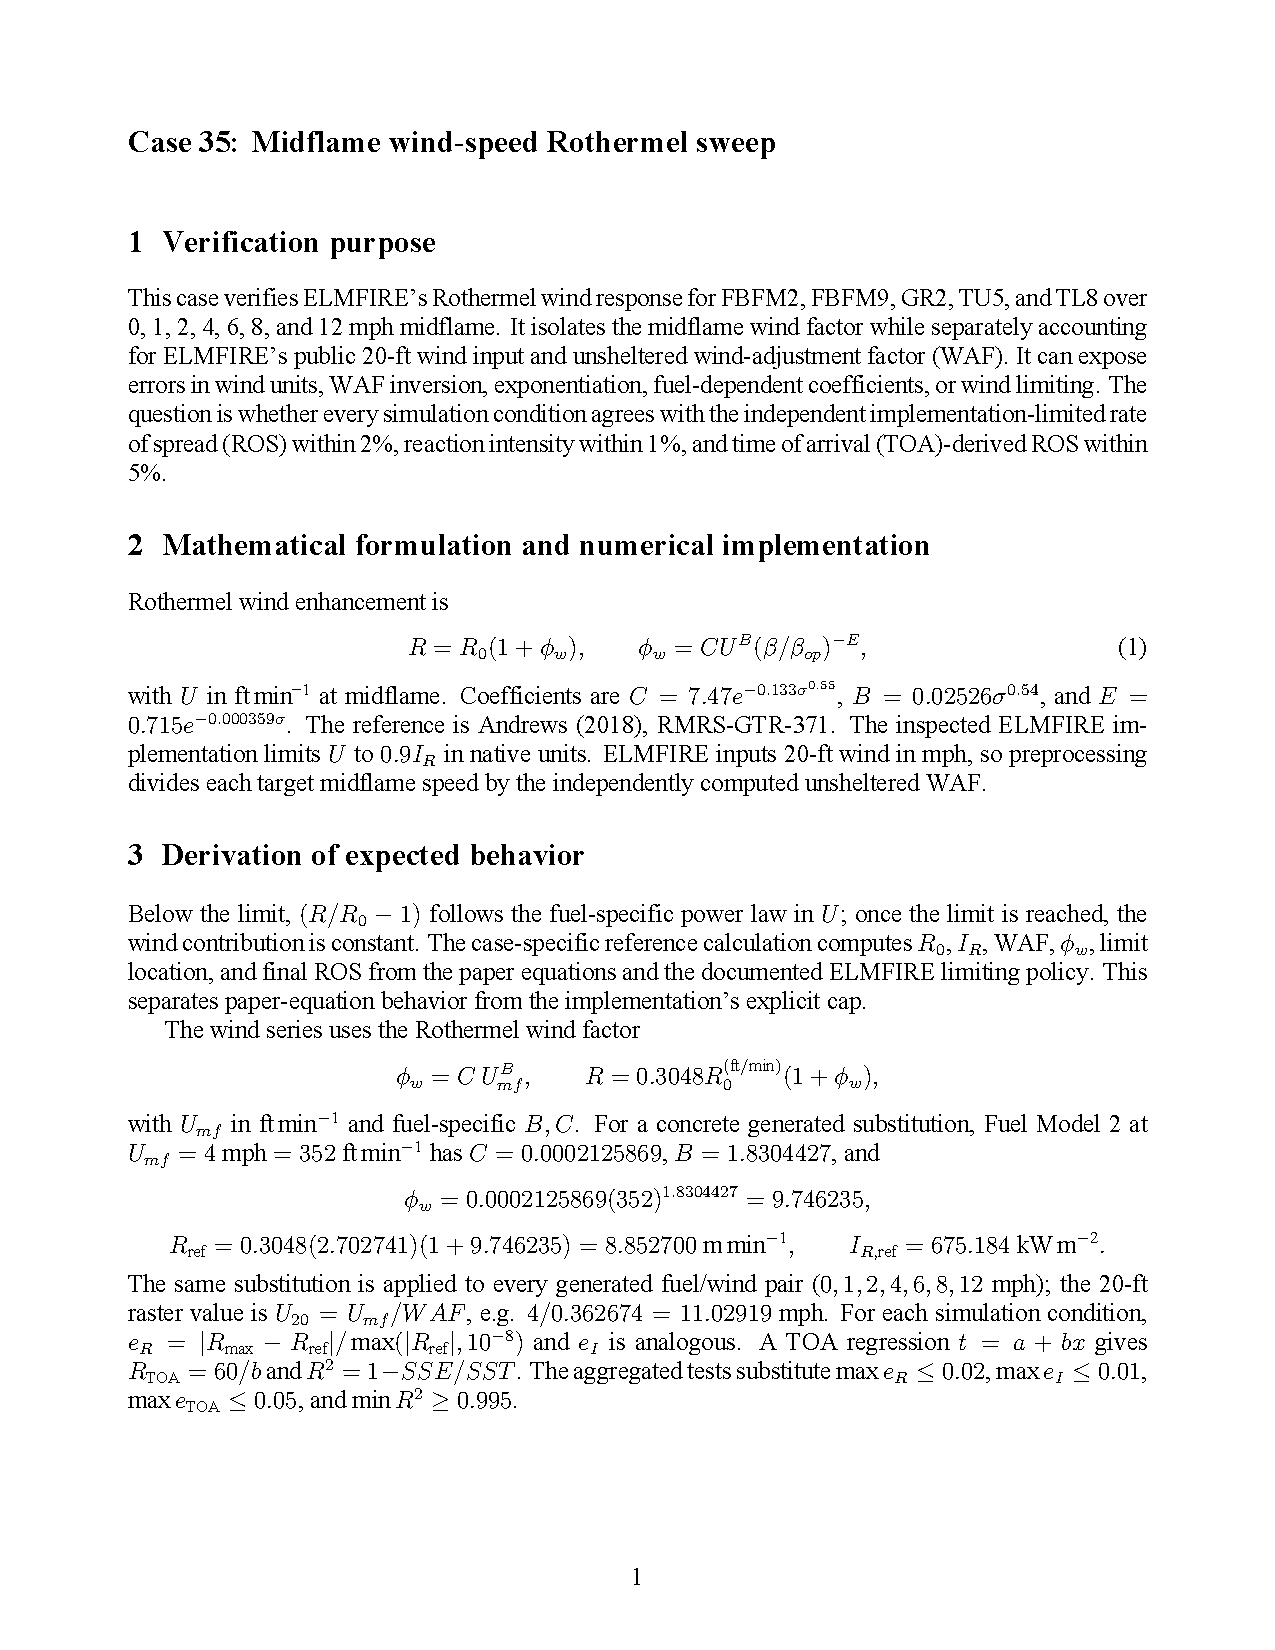
\includepdf[pages=-,pagecommand={\thispagestyle{empty}},addtotoc={1,section,1,{CASE35\_WSS -- Case 35: Midflame wind-speed Rothermel sweep},case-detail:case35-wss}]{../cases/Verification/unit_tests/CASE35_WSS/report/case_report.pdf}%
}{%
  \phantomsection
  \label{case-detail:case35-wss}
  \addcontentsline{toc}{section}{CASE35\_WSS -- Case 35: Midflame wind-speed Rothermel sweep}
  \section*{CASE35\_WSS -- Case 35: Midflame wind-speed Rothermel sweep}
  \textbf{NOT EVALUABLE:} the detailed case description is unavailable.
}

\clearpage
\IfFileExists{../cases/Verification/unit_tests/CASE36_SLS/report/case_report.pdf}{%
  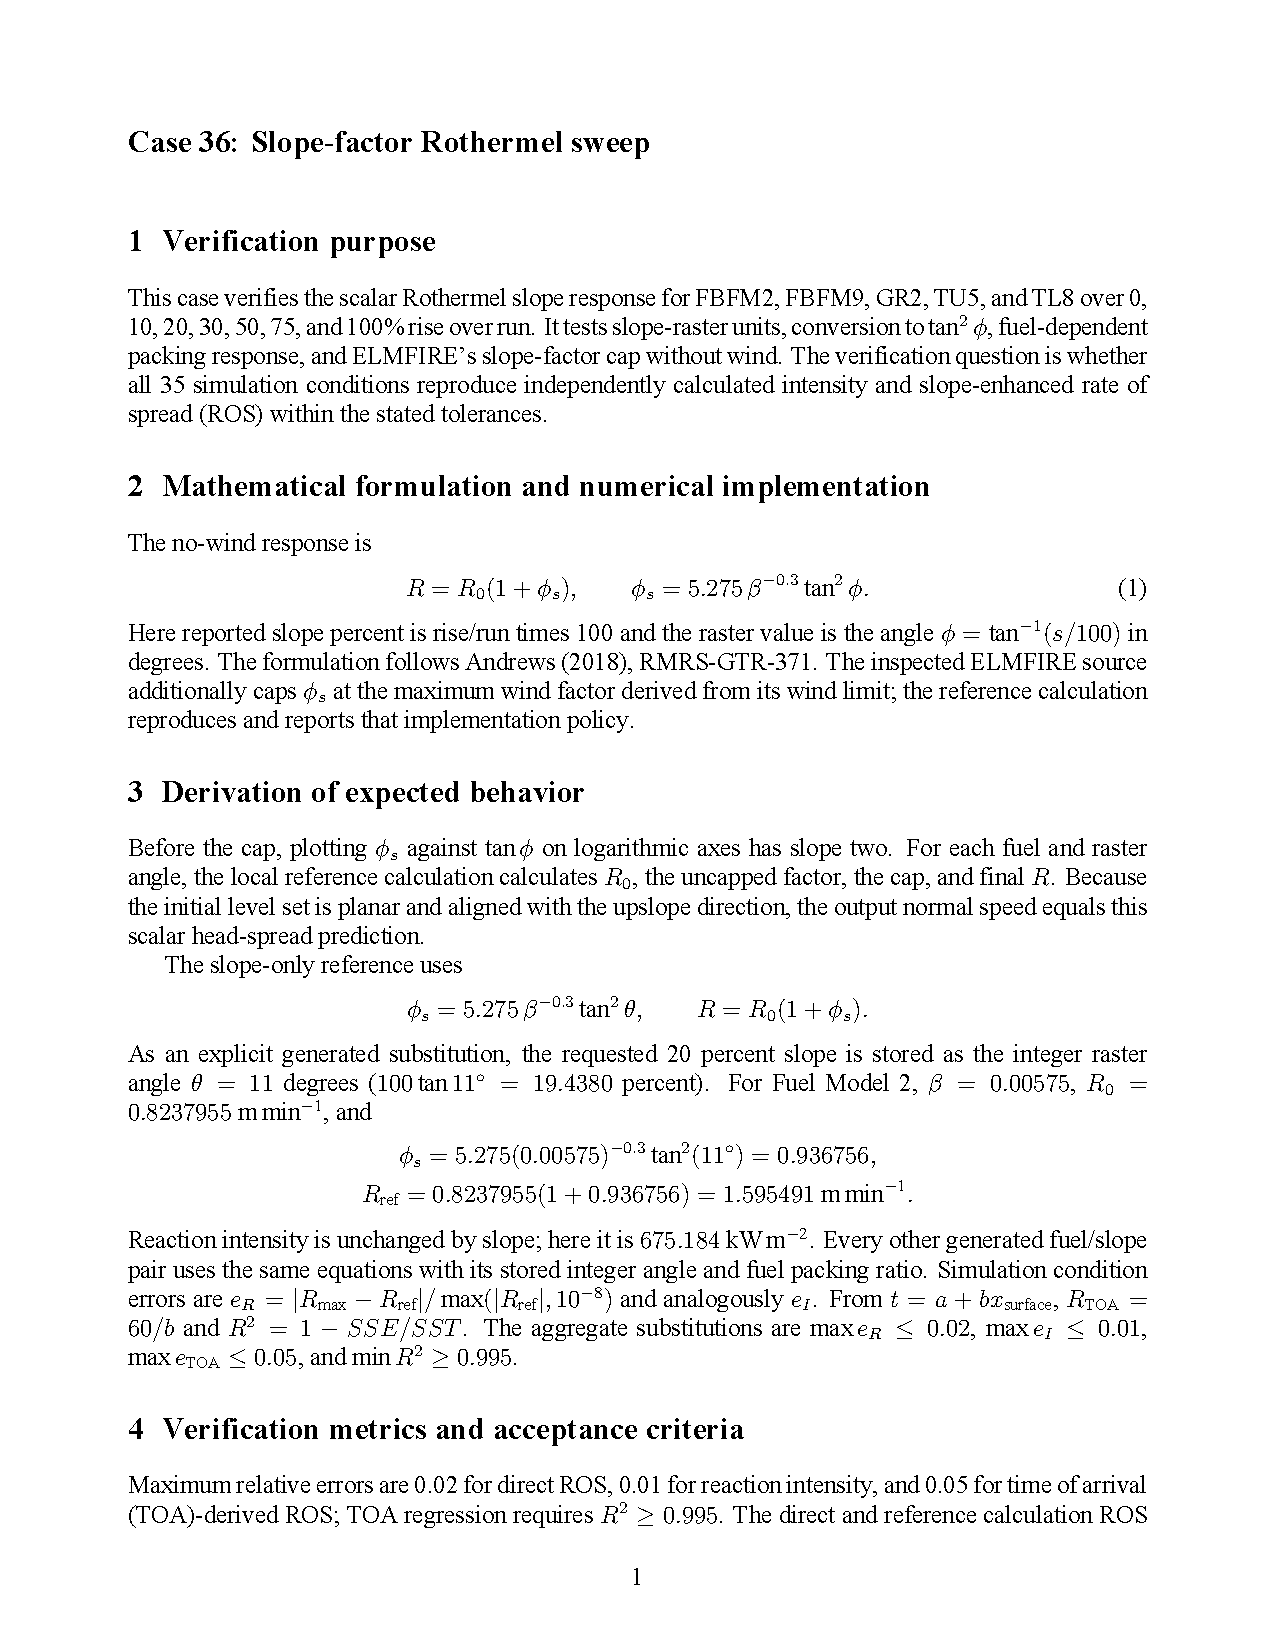
\includepdf[pages=-,pagecommand={\thispagestyle{empty}},addtotoc={1,section,1,{CASE36\_SLS -- Case 36: Slope-factor Rothermel sweep},case-detail:case36-sls}]{../cases/Verification/unit_tests/CASE36_SLS/report/case_report.pdf}%
}{%
  \phantomsection
  \label{case-detail:case36-sls}
  \addcontentsline{toc}{section}{CASE36\_SLS -- Case 36: Slope-factor Rothermel sweep}
  \section*{CASE36\_SLS -- Case 36: Slope-factor Rothermel sweep}
  \textbf{NOT EVALUABLE:} the detailed case description is unavailable.
}

\clearpage
\IfFileExists{../cases/Verification/unit_tests/CASE37_DMS/report/case_report.pdf}{%
  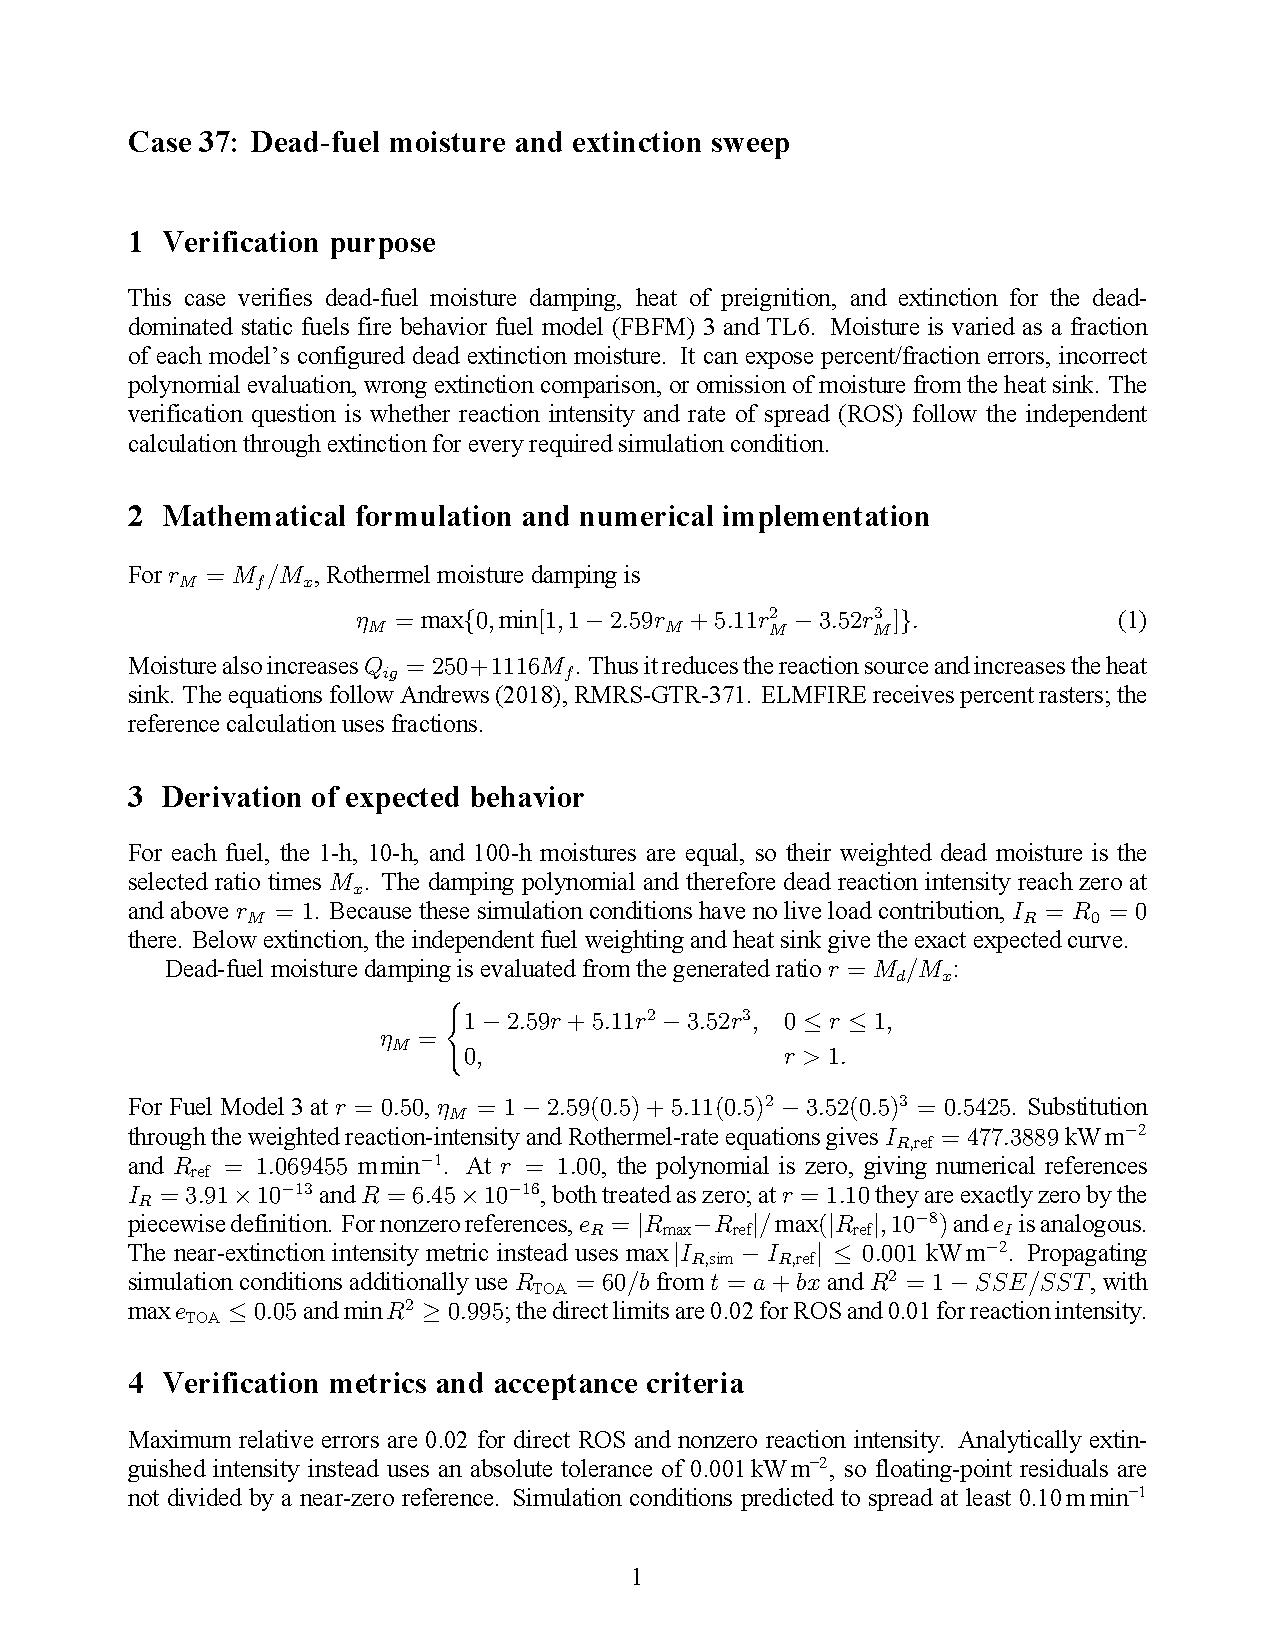
\includepdf[pages=-,pagecommand={\thispagestyle{empty}},addtotoc={1,section,1,{CASE37\_DMS -- Case 37: Dead-fuel moisture and extinction sweep},case-detail:case37-dms}]{../cases/Verification/unit_tests/CASE37_DMS/report/case_report.pdf}%
}{%
  \phantomsection
  \label{case-detail:case37-dms}
  \addcontentsline{toc}{section}{CASE37\_DMS -- Case 37: Dead-fuel moisture and extinction sweep}
  \section*{CASE37\_DMS -- Case 37: Dead-fuel moisture and extinction sweep}
  \textbf{NOT EVALUABLE:} the detailed case description is unavailable.
}

\clearpage
\IfFileExists{../cases/Verification/unit_tests/CASE38_LMS/report/case_report.pdf}{%
  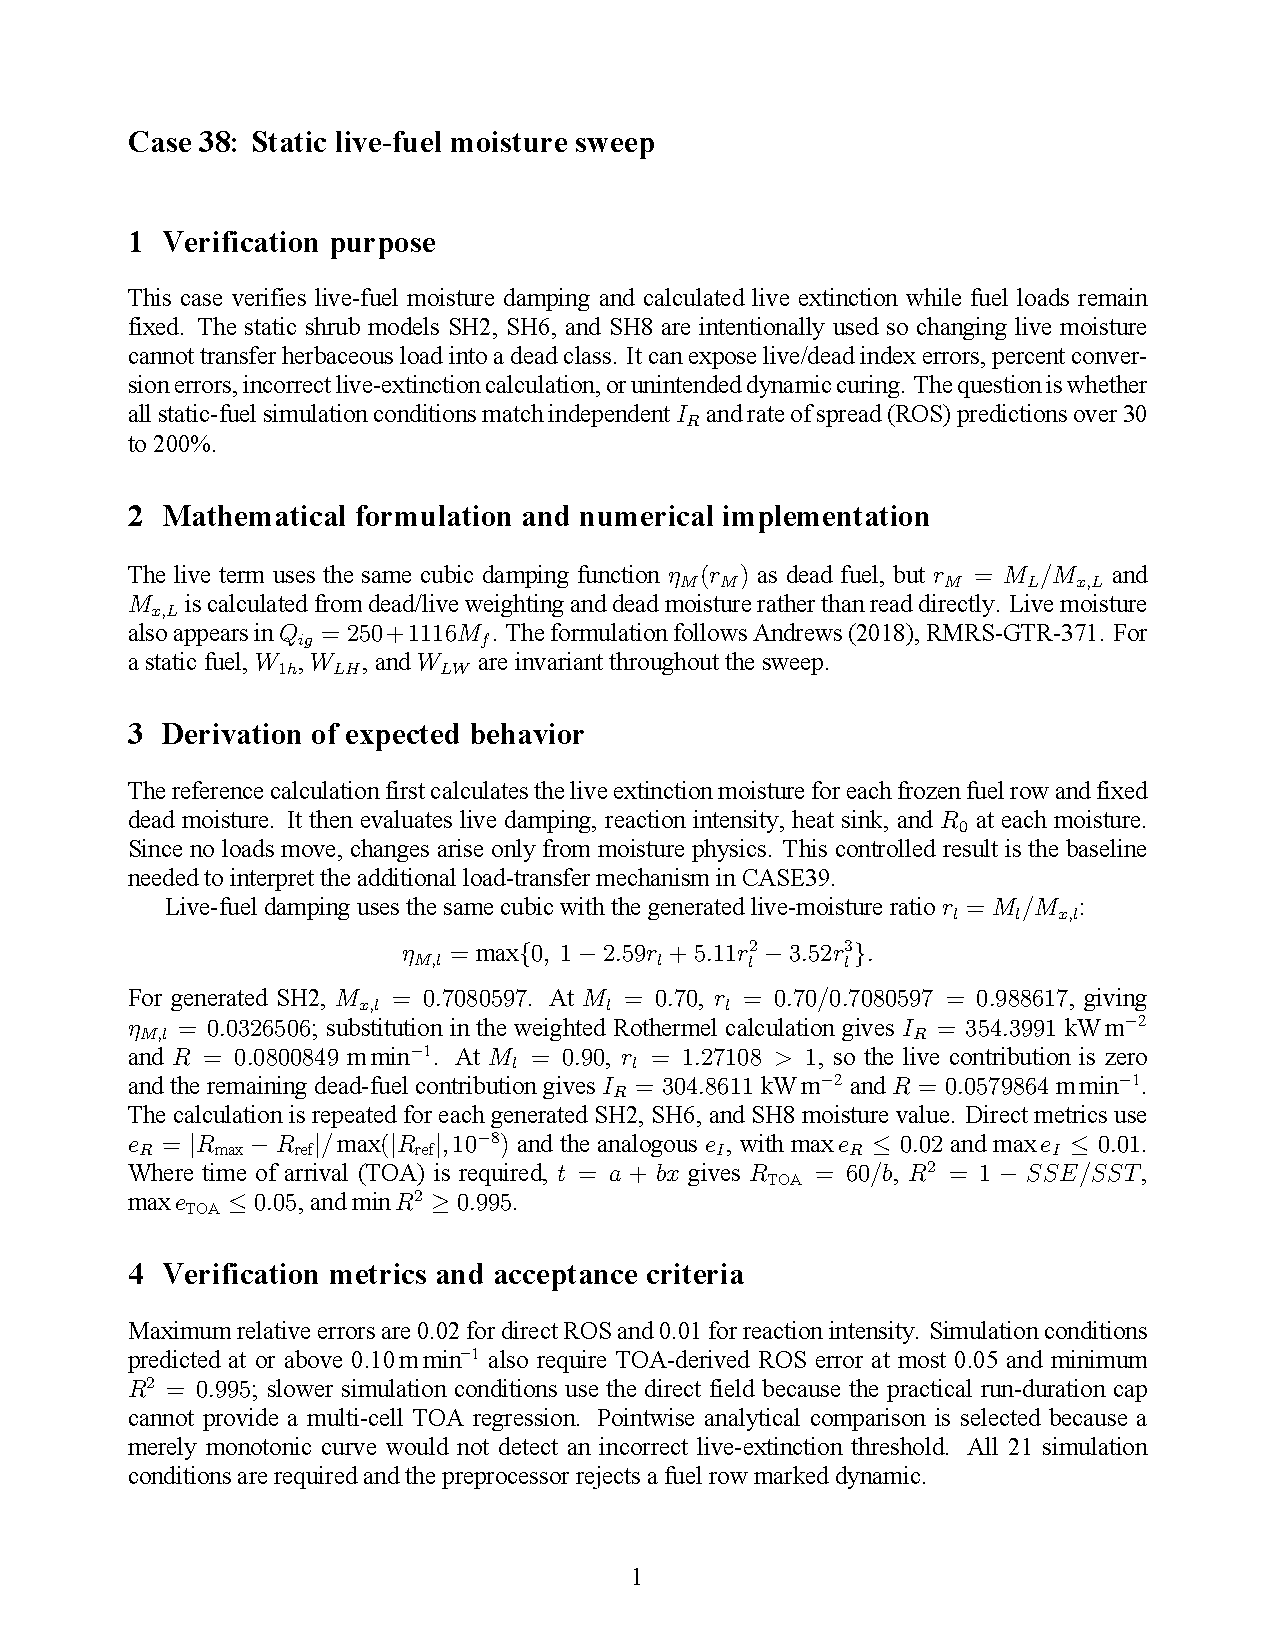
\includepdf[pages=-,pagecommand={\thispagestyle{empty}},addtotoc={1,section,1,{CASE38\_LMS -- Case 38: Static live-fuel moisture sweep},case-detail:case38-lms}]{../cases/Verification/unit_tests/CASE38_LMS/report/case_report.pdf}%
}{%
  \phantomsection
  \label{case-detail:case38-lms}
  \addcontentsline{toc}{section}{CASE38\_LMS -- Case 38: Static live-fuel moisture sweep}
  \section*{CASE38\_LMS -- Case 38: Static live-fuel moisture sweep}
  \textbf{NOT EVALUABLE:} the detailed case description is unavailable.
}

\clearpage
\IfFileExists{../cases/Verification/unit_tests/CASE39_DHC/report/case_report.pdf}{%
  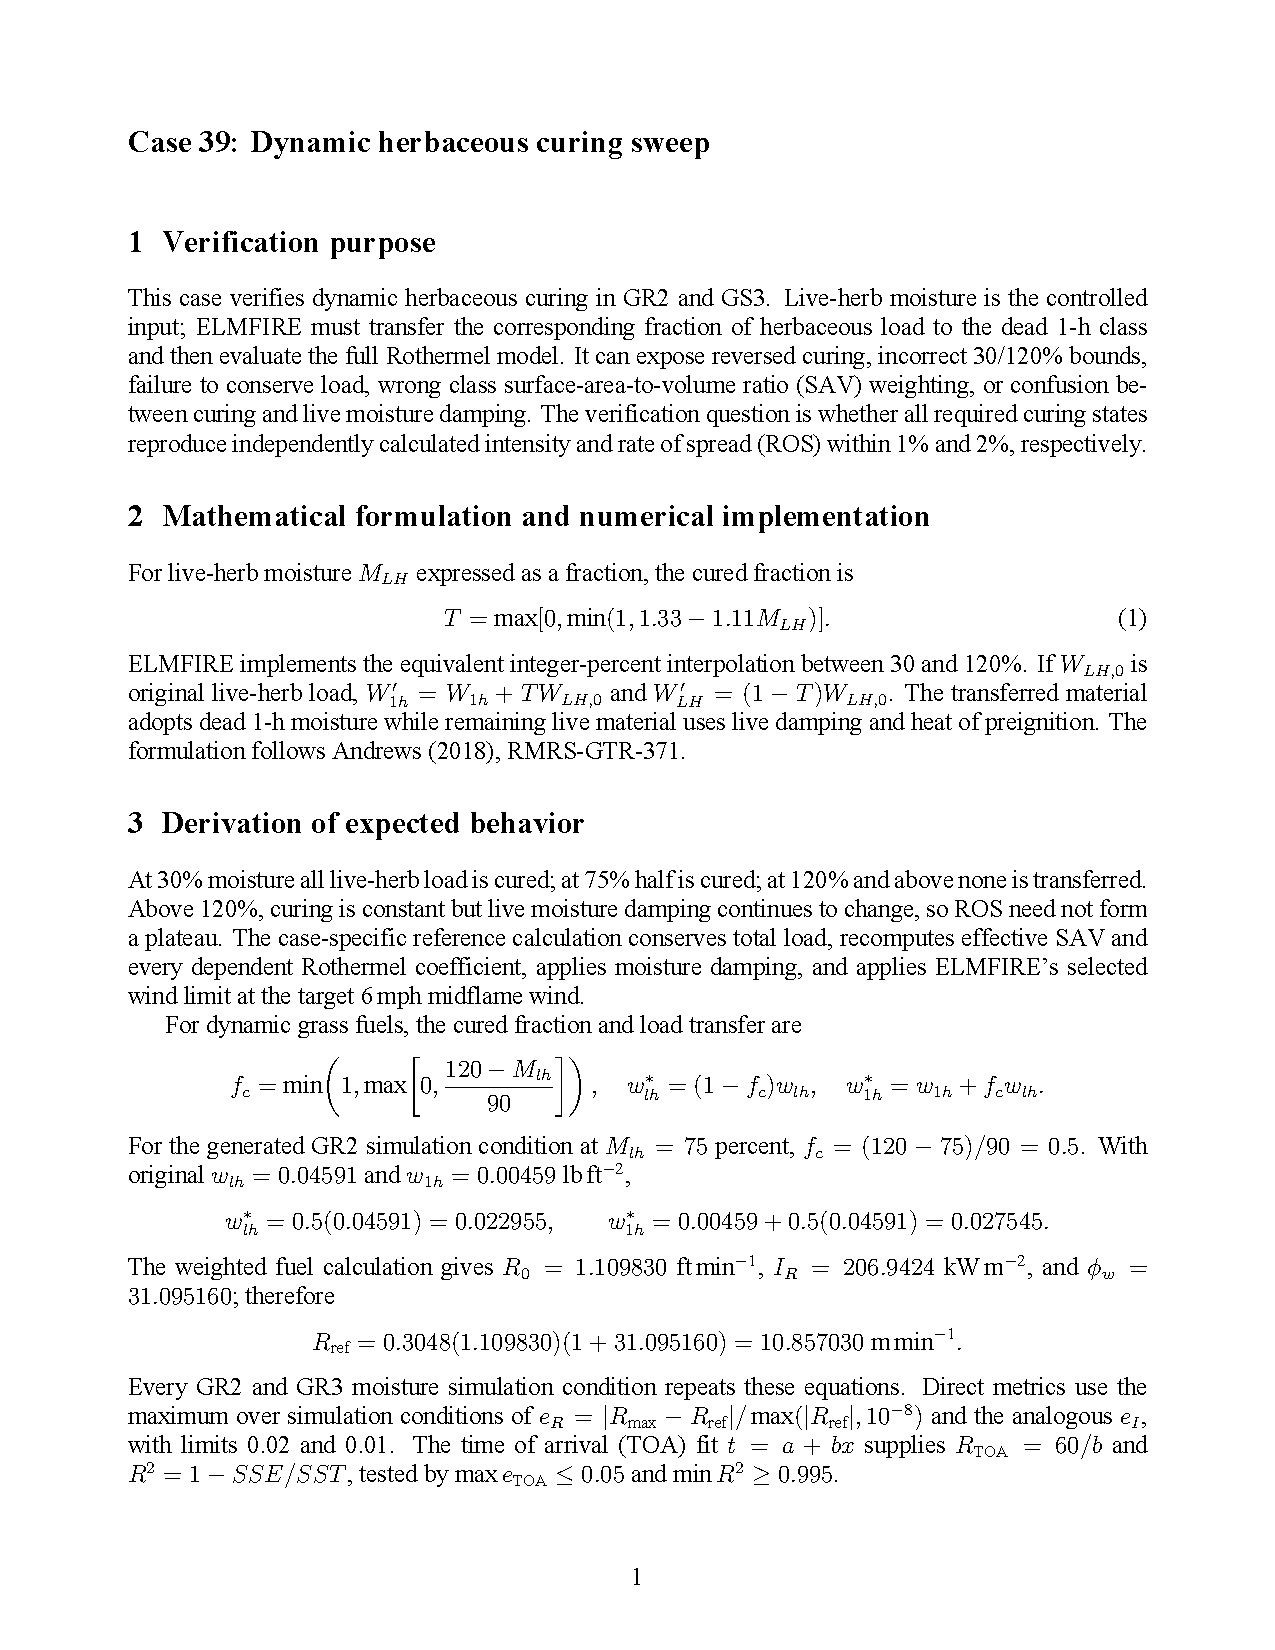
\includepdf[pages=-,pagecommand={\thispagestyle{empty}},addtotoc={1,section,1,{CASE39\_DHC -- Case 39: Dynamic herbaceous curing sweep},case-detail:case39-dhc}]{../cases/Verification/unit_tests/CASE39_DHC/report/case_report.pdf}%
}{%
  \phantomsection
  \label{case-detail:case39-dhc}
  \addcontentsline{toc}{section}{CASE39\_DHC -- Case 39: Dynamic herbaceous curing sweep}
  \section*{CASE39\_DHC -- Case 39: Dynamic herbaceous curing sweep}
  \textbf{NOT EVALUABLE:} the detailed case description is unavailable.
}

\clearpage
\IfFileExists{../cases/Verification/coupling_tests/CASE40_WSD/report/case_report.pdf}{%
  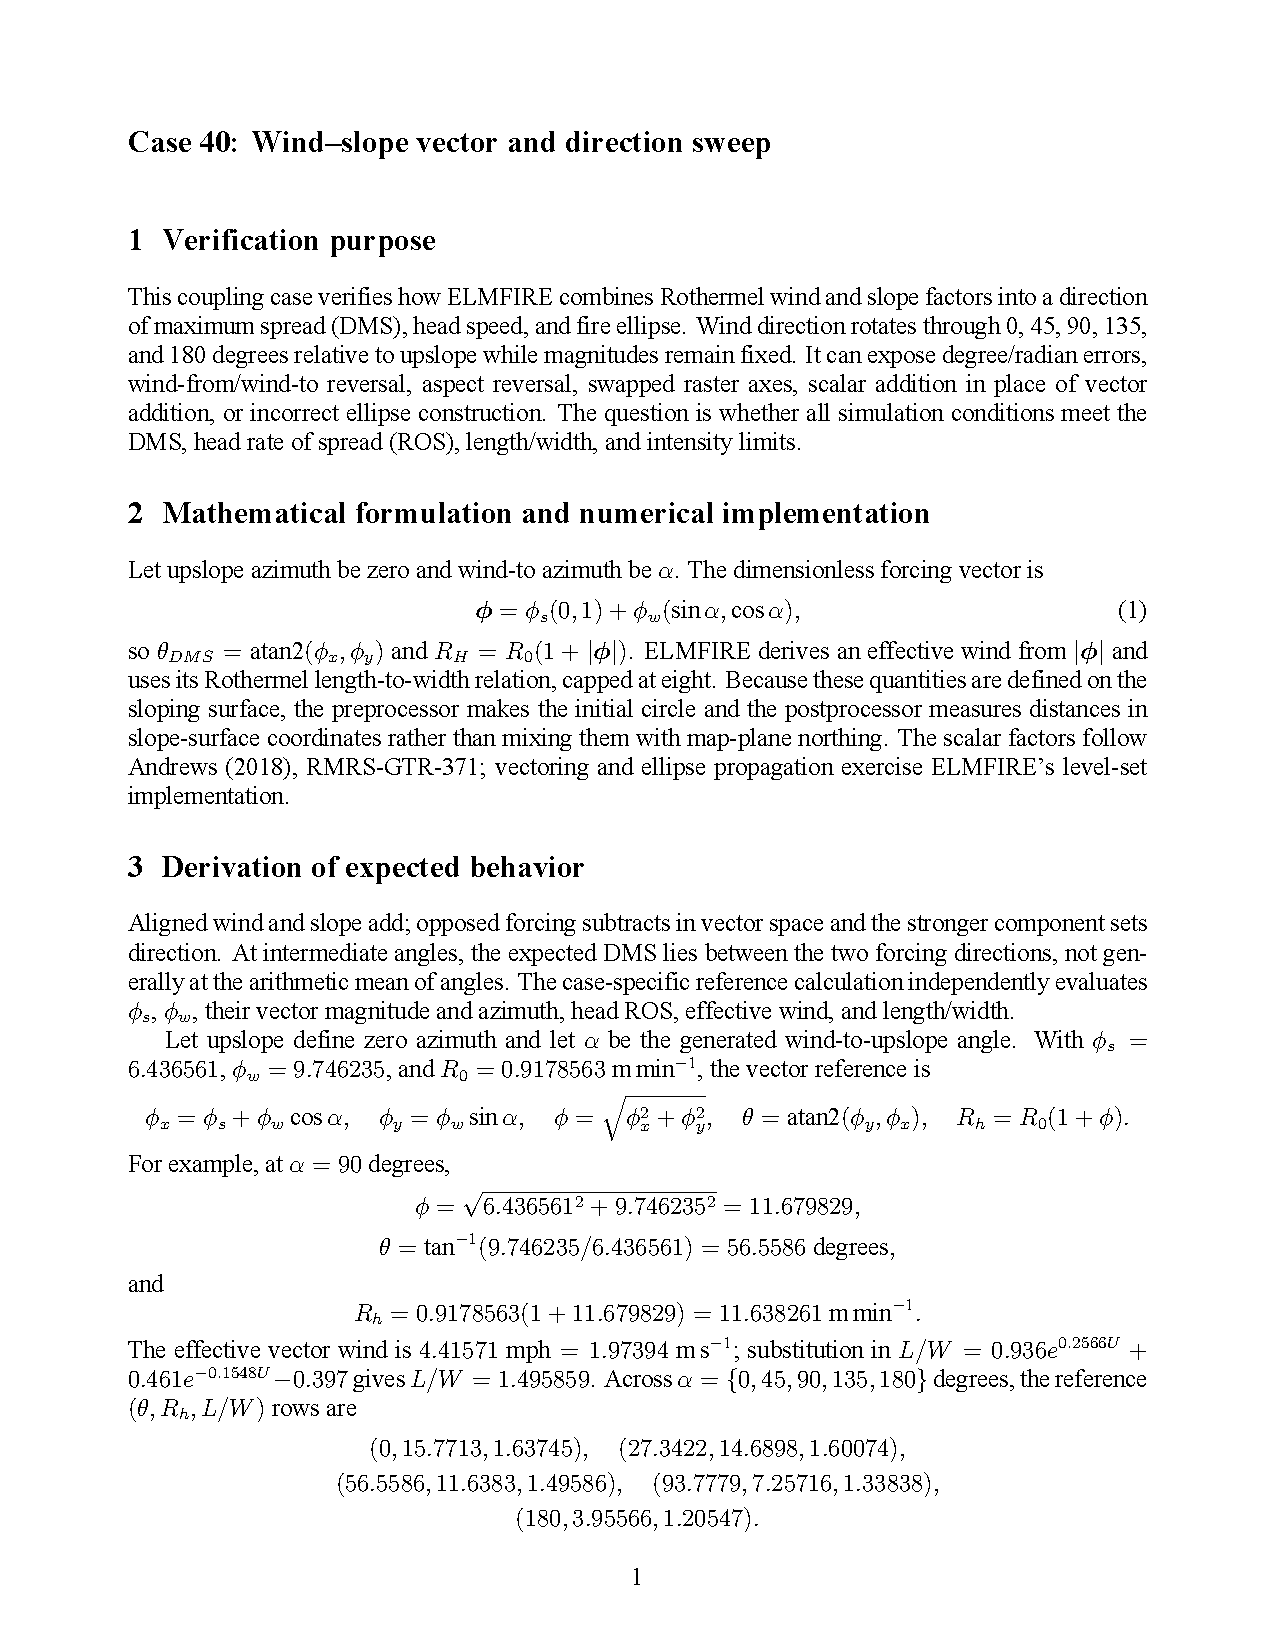
\includepdf[pages=-,pagecommand={\thispagestyle{empty}},addtotoc={1,section,1,{CASE40\_WSD -- Case 40: Wind-slope vector and direction sweep},case-detail:case40-wsd}]{../cases/Verification/coupling_tests/CASE40_WSD/report/case_report.pdf}%
}{%
  \phantomsection
  \label{case-detail:case40-wsd}
  \addcontentsline{toc}{section}{CASE40\_WSD -- Case 40: Wind-slope vector and direction sweep}
  \section*{CASE40\_WSD -- Case 40: Wind-slope vector and direction sweep}
  \textbf{NOT EVALUABLE:} the detailed case description is unavailable.
}

\clearpage
\IfFileExists{../cases/Verification/unit_tests/CASE41_CFP/report/case_report.pdf}{%
  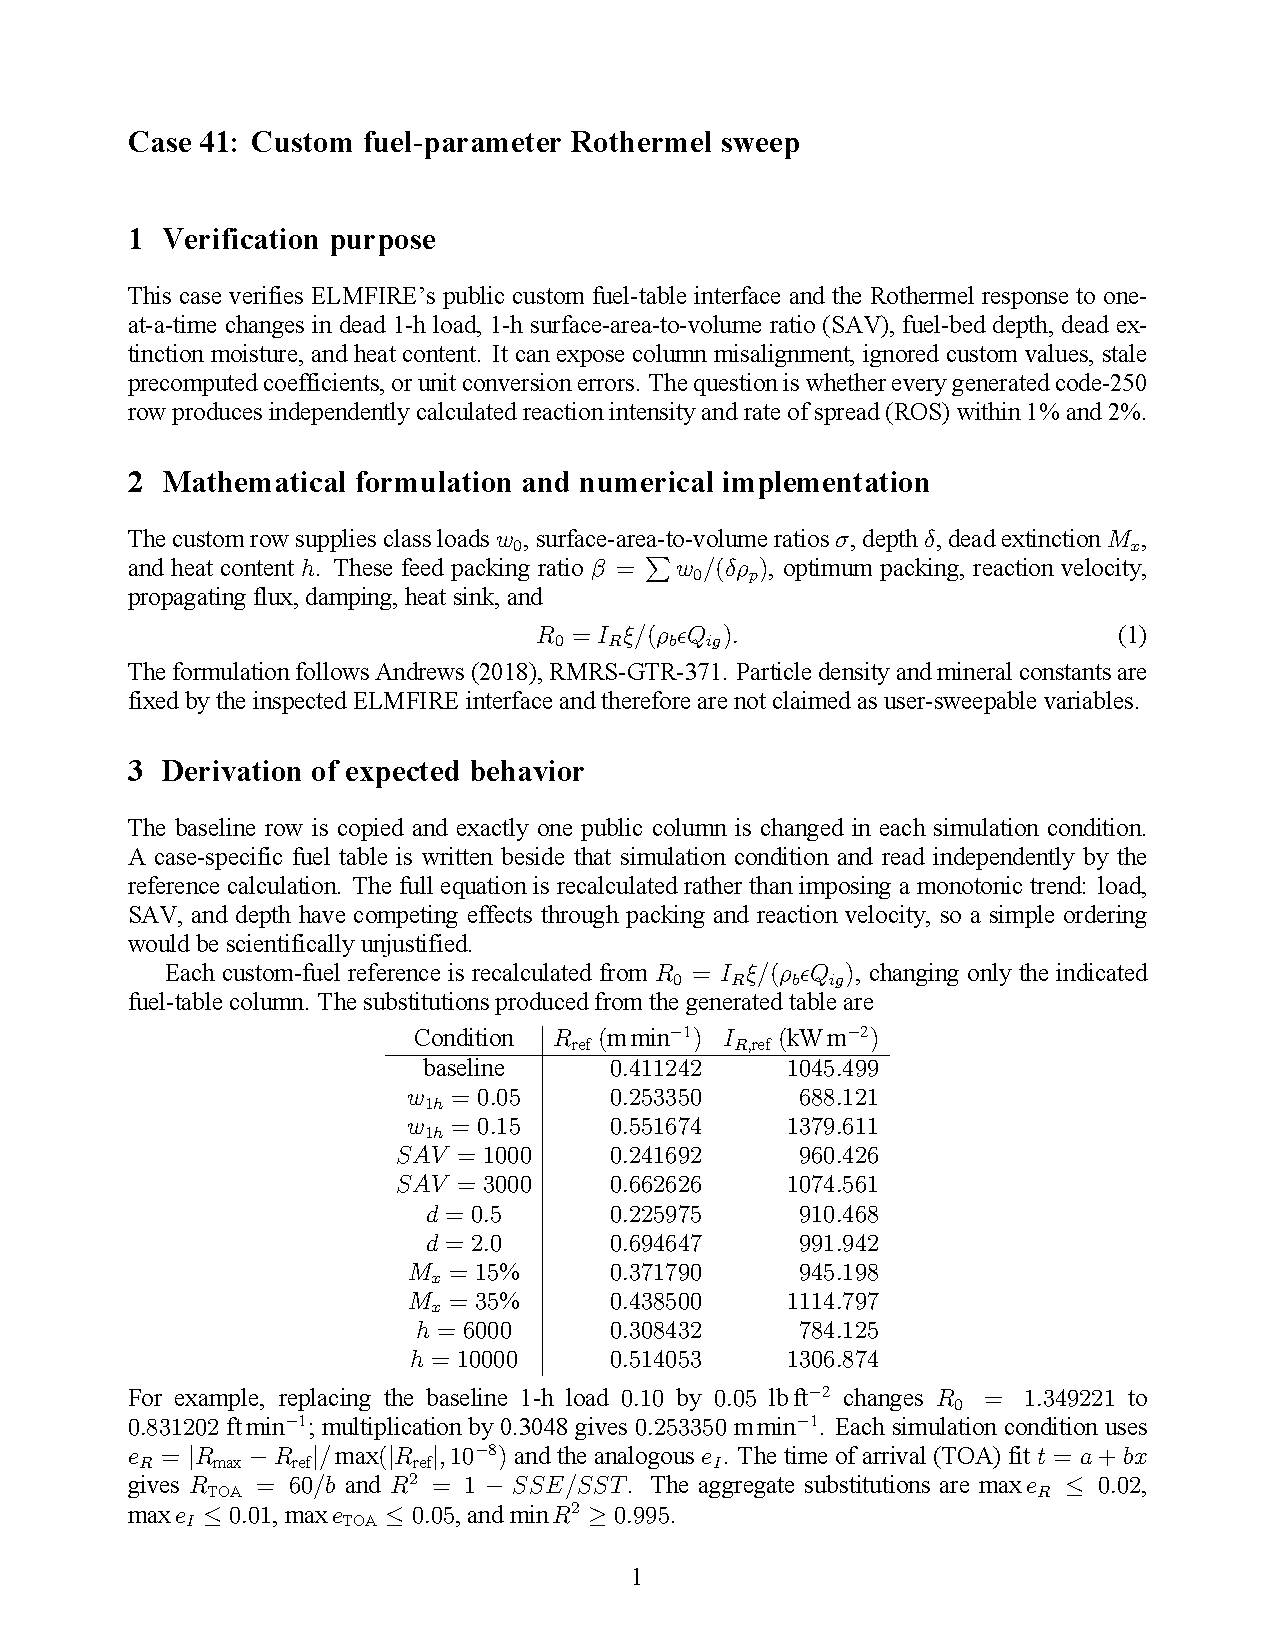
\includepdf[pages=-,pagecommand={\thispagestyle{empty}},addtotoc={1,section,1,{CASE41\_CFP -- Case 41: Custom fuel-parameter Rothermel sweep},case-detail:case41-cfp}]{../cases/Verification/unit_tests/CASE41_CFP/report/case_report.pdf}%
}{%
  \phantomsection
  \label{case-detail:case41-cfp}
  \addcontentsline{toc}{section}{CASE41\_CFP -- Case 41: Custom fuel-parameter Rothermel sweep}
  \section*{CASE41\_CFP -- Case 41: Custom fuel-parameter Rothermel sweep}
  \textbf{NOT EVALUABLE:} the detailed case description is unavailable.
}

\clearpage
\IfFileExists{../cases/Verification/coupling_tests/CASE42_WAF/report/case_report.pdf}{%
  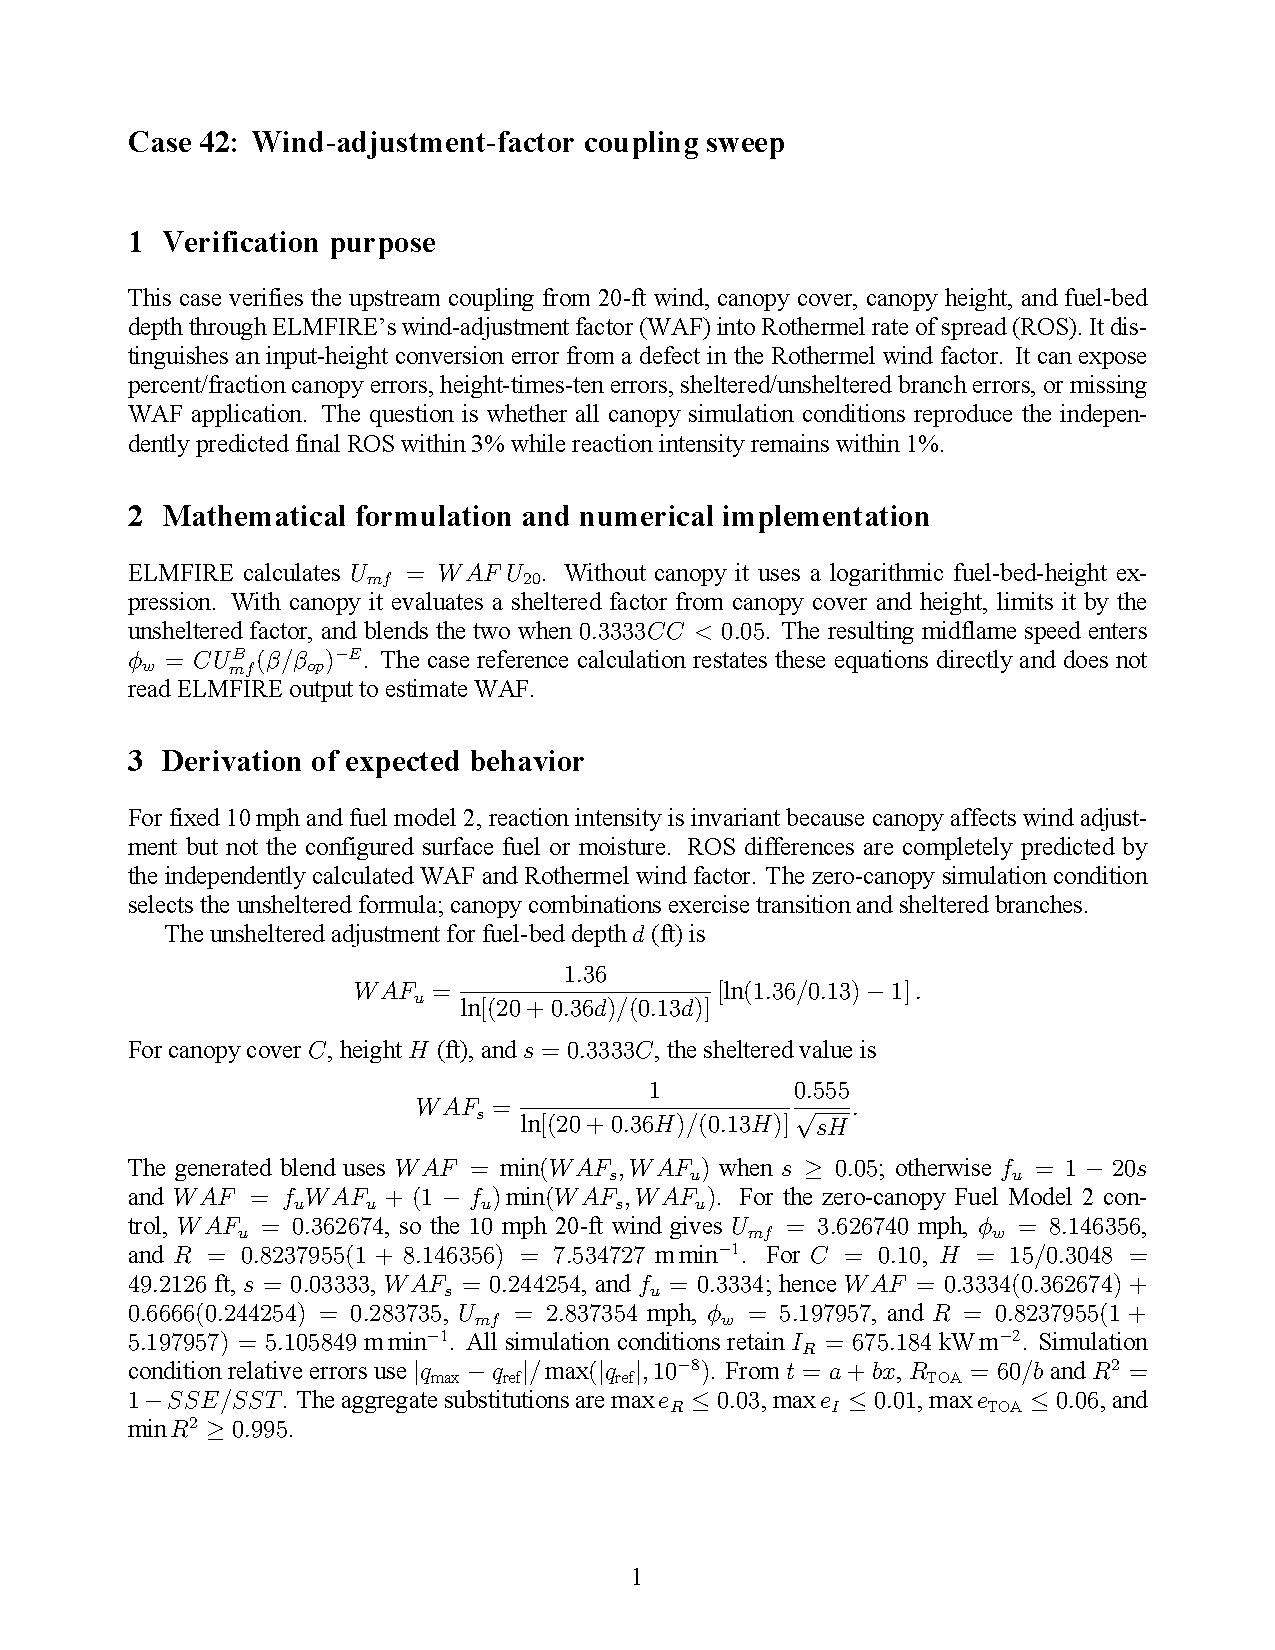
\includepdf[pages=-,pagecommand={\thispagestyle{empty}},addtotoc={1,section,1,{CASE42\_WAF -- Case 42: Wind-adjustment-factor coupling sweep},case-detail:case42-waf}]{../cases/Verification/coupling_tests/CASE42_WAF/report/case_report.pdf}%
}{%
  \phantomsection
  \label{case-detail:case42-waf}
  \addcontentsline{toc}{section}{CASE42\_WAF -- Case 42: Wind-adjustment-factor coupling sweep}
  \section*{CASE42\_WAF -- Case 42: Wind-adjustment-factor coupling sweep}
  \textbf{NOT EVALUABLE:} the detailed case description is unavailable.
}

\clearpage
\IfFileExists{../cases/Verification/coupling_tests/CASE43_WER/report/case_report.pdf}{%
  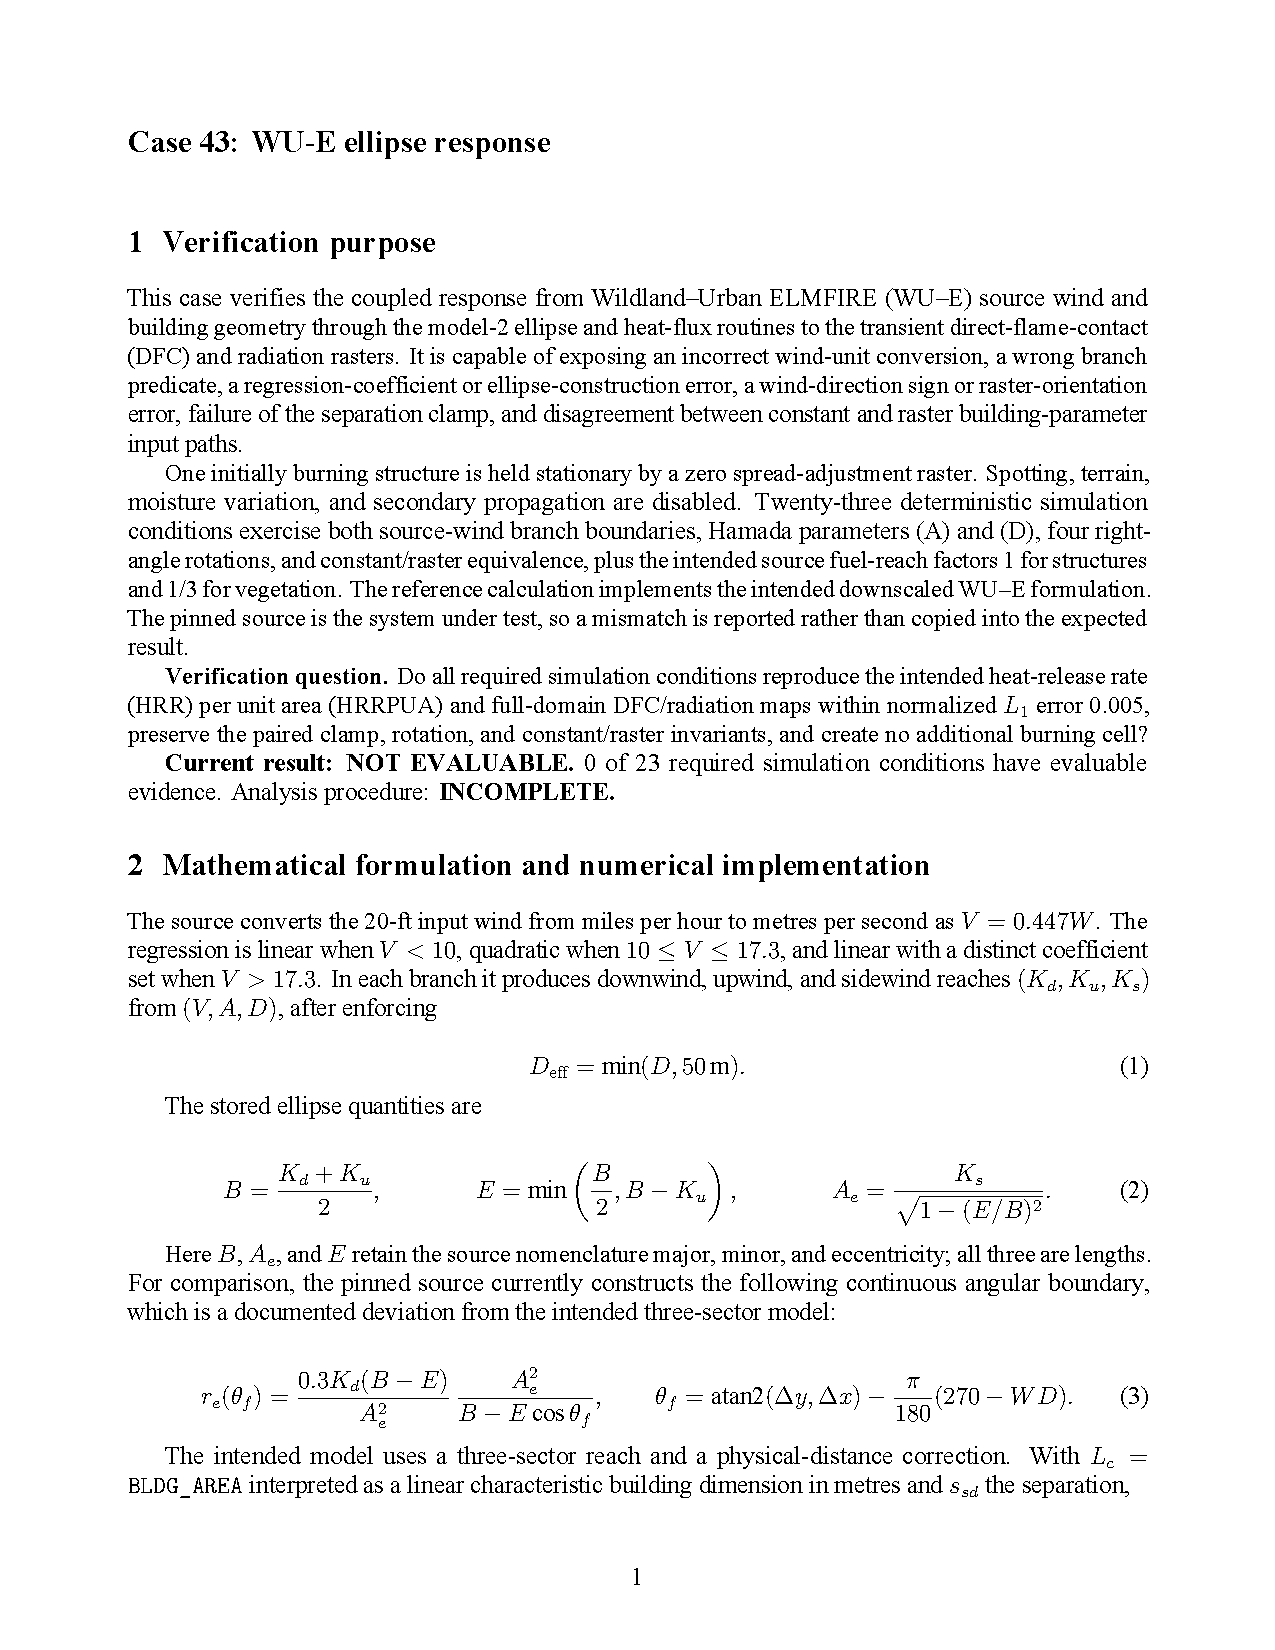
\includepdf[pages=-,pagecommand={\thispagestyle{empty}},addtotoc={1,section,1,{CASE43\_WER -- Case 43: WU-E ellipse response},case-detail:case43-wer}]{../cases/Verification/coupling_tests/CASE43_WER/report/case_report.pdf}%
}{%
  \phantomsection
  \label{case-detail:case43-wer}
  \addcontentsline{toc}{section}{CASE43\_WER -- Case 43: WU-E ellipse response}
  \section*{CASE43\_WER -- Case 43: WU-E ellipse response}
  \textbf{NOT EVALUABLE:} the detailed case description is unavailable.
}

\clearpage
\IfFileExists{../cases/Verification/coupling_tests/CASE44_WHP/report/case_report.pdf}{%
  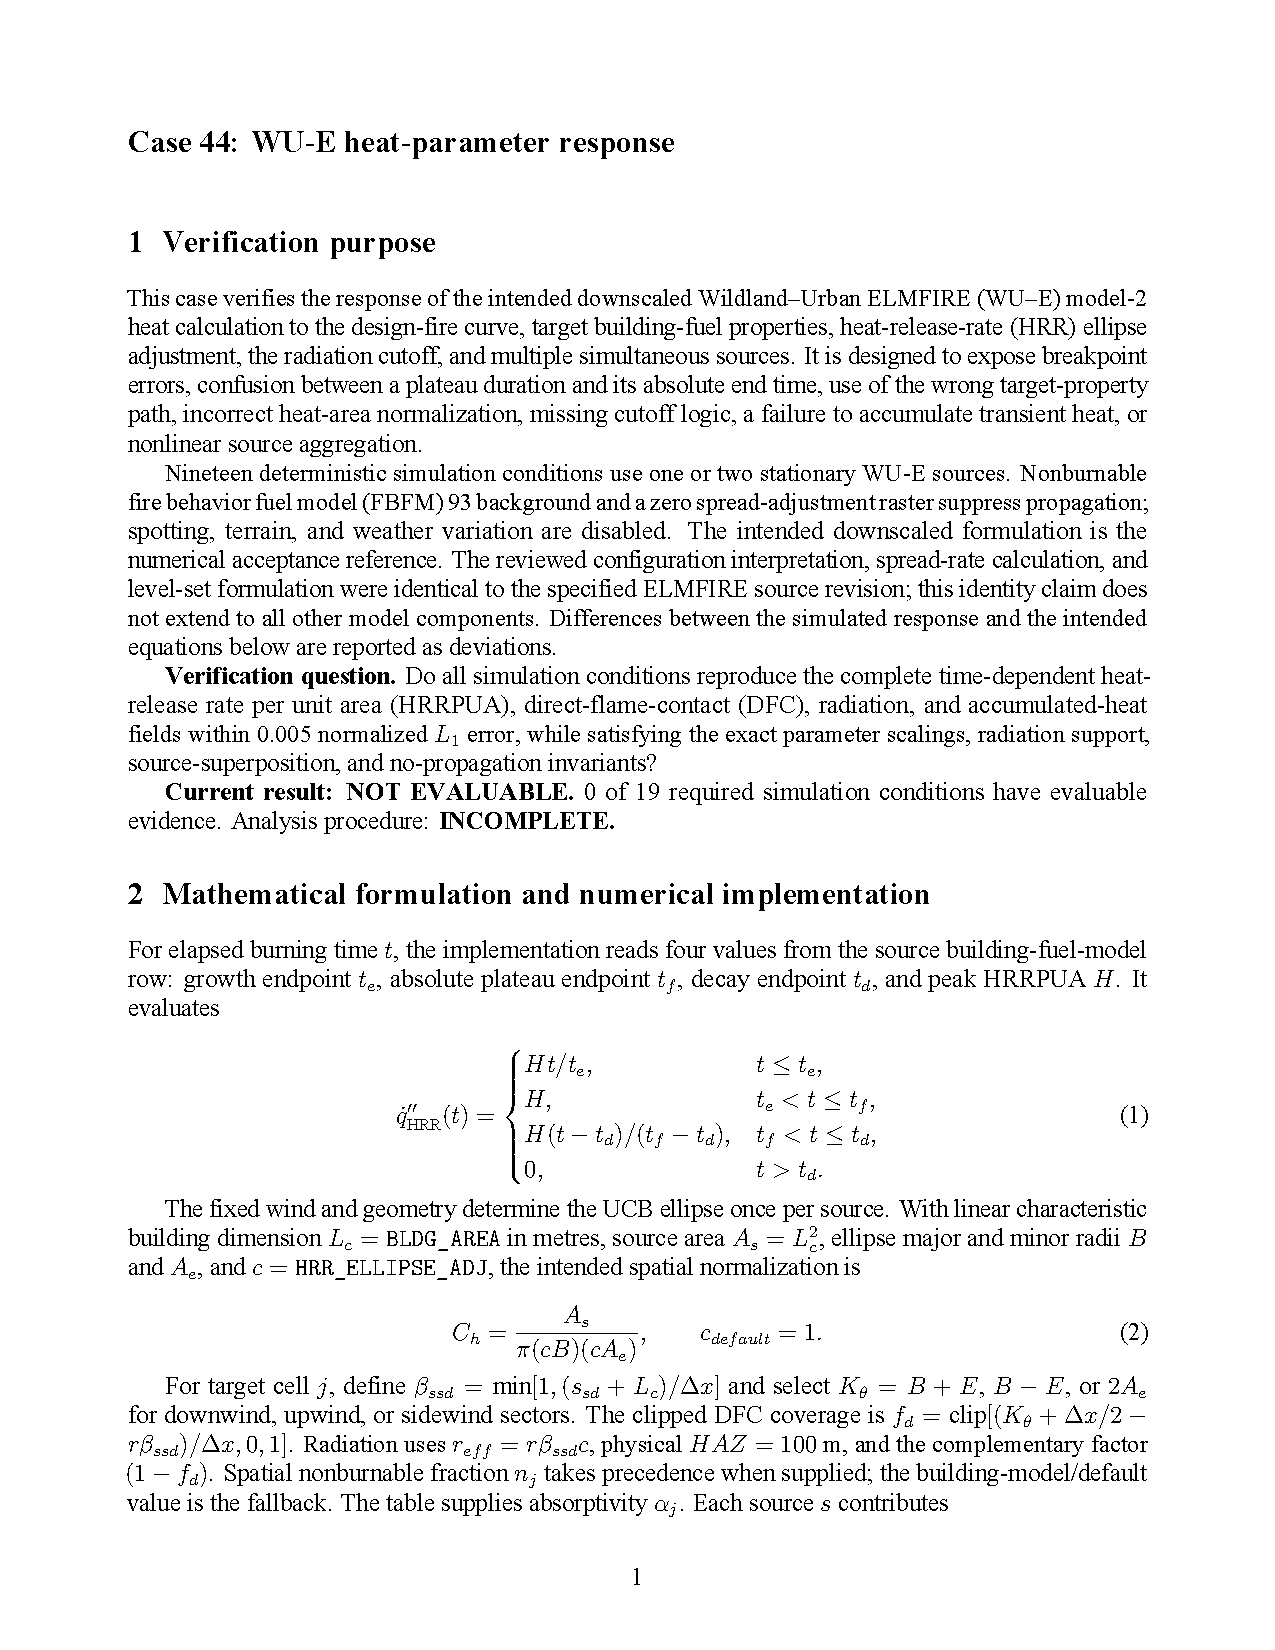
\includepdf[pages=-,pagecommand={\thispagestyle{empty}},addtotoc={1,section,1,{CASE44\_WHP -- Case 44: WU-E heat-parameter response},case-detail:case44-whp}]{../cases/Verification/coupling_tests/CASE44_WHP/report/case_report.pdf}%
}{%
  \phantomsection
  \label{case-detail:case44-whp}
  \addcontentsline{toc}{section}{CASE44\_WHP -- Case 44: WU-E heat-parameter response}
  \section*{CASE44\_WHP -- Case 44: WU-E heat-parameter response}
  \textbf{NOT EVALUABLE:} the detailed case description is unavailable.
}

\clearpage
\IfFileExists{../cases/Verification/coupling_tests/CASE45_HRS/report/case_report.pdf}{%
  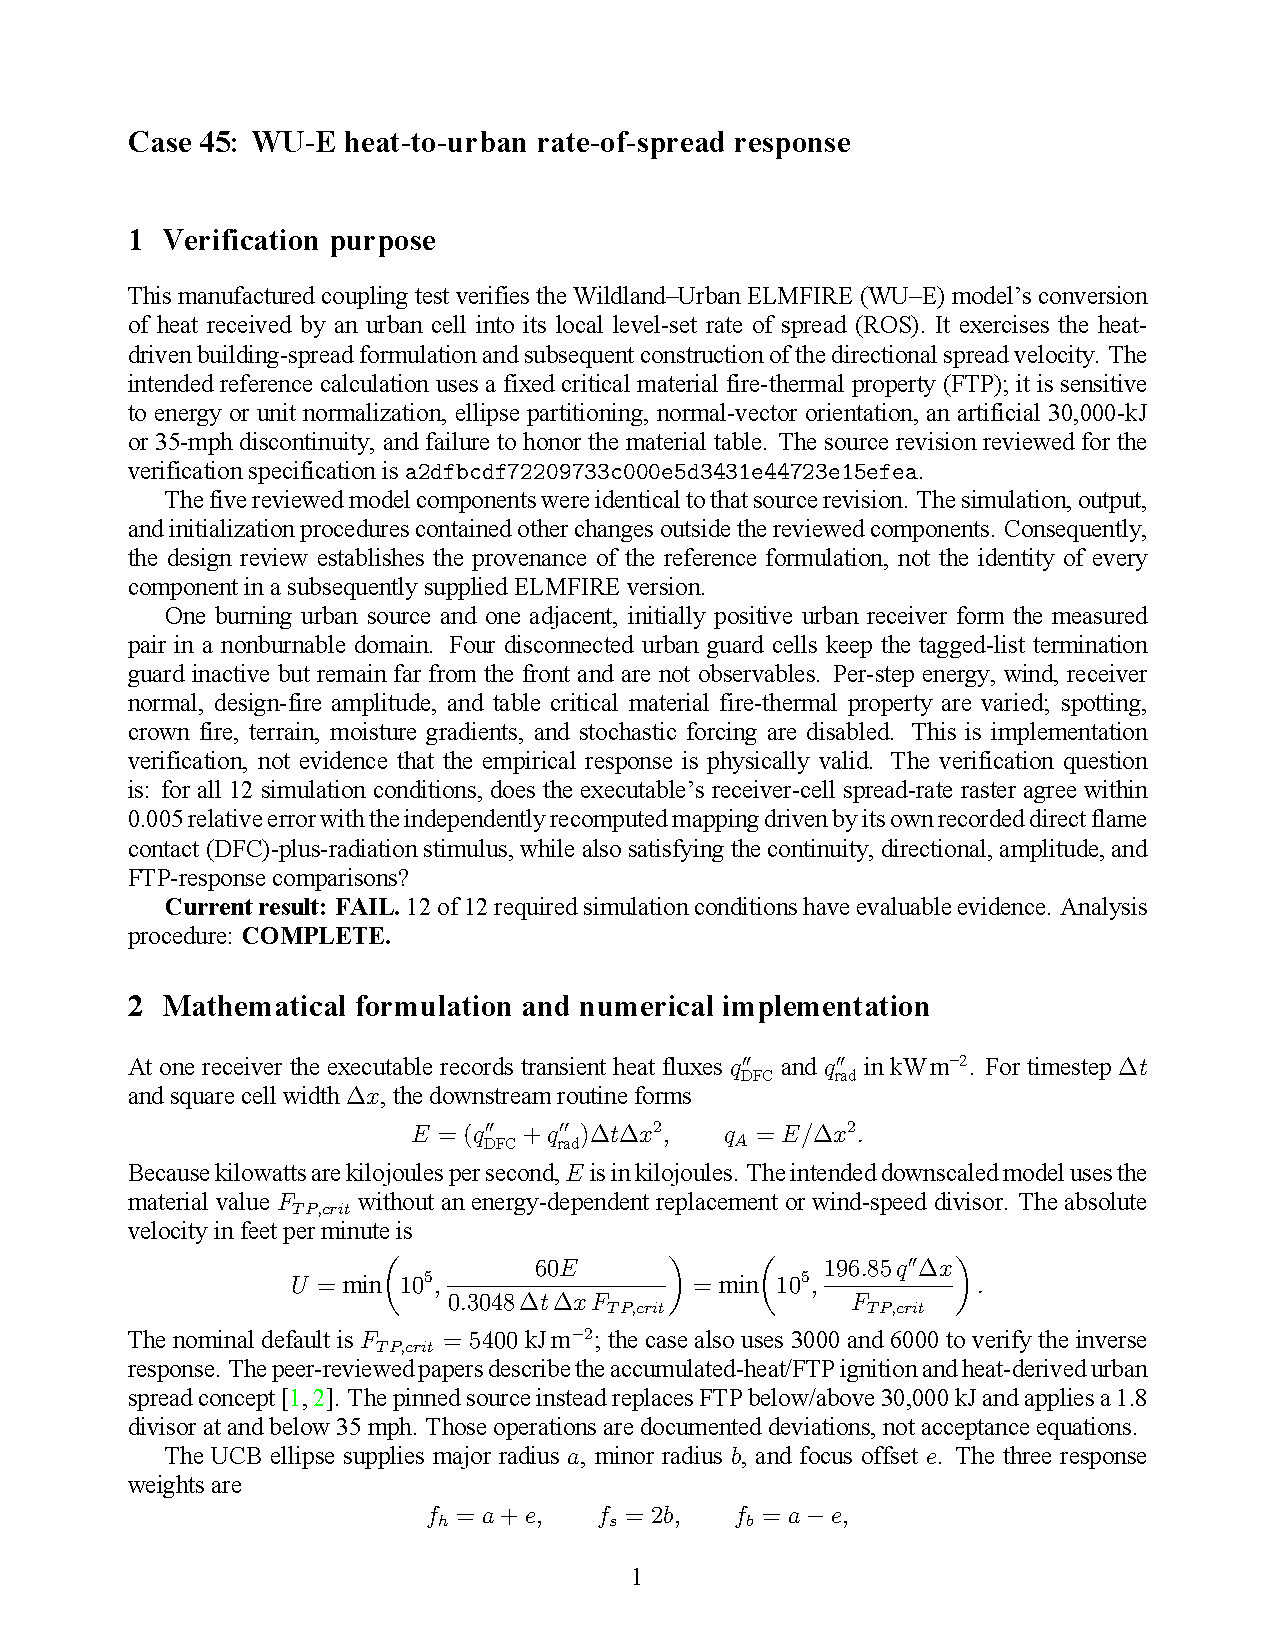
\includepdf[pages=-,pagecommand={\thispagestyle{empty}},addtotoc={1,section,1,{CASE45\_HRS -- Case 45: WU-E heat-to-urban rate-of-spread response},case-detail:case45-hrs}]{../cases/Verification/coupling_tests/CASE45_HRS/report/case_report.pdf}%
}{%
  \phantomsection
  \label{case-detail:case45-hrs}
  \addcontentsline{toc}{section}{CASE45\_HRS -- Case 45: WU-E heat-to-urban rate-of-spread response}
  \section*{CASE45\_HRS -- Case 45: WU-E heat-to-urban rate-of-spread response}
  \textbf{NOT EVALUABLE:} the detailed case description is unavailable.
}

\clearpage
\IfFileExists{../cases/Verification/coupling_tests/CASE46_WUT/report/case_report.pdf}{%
  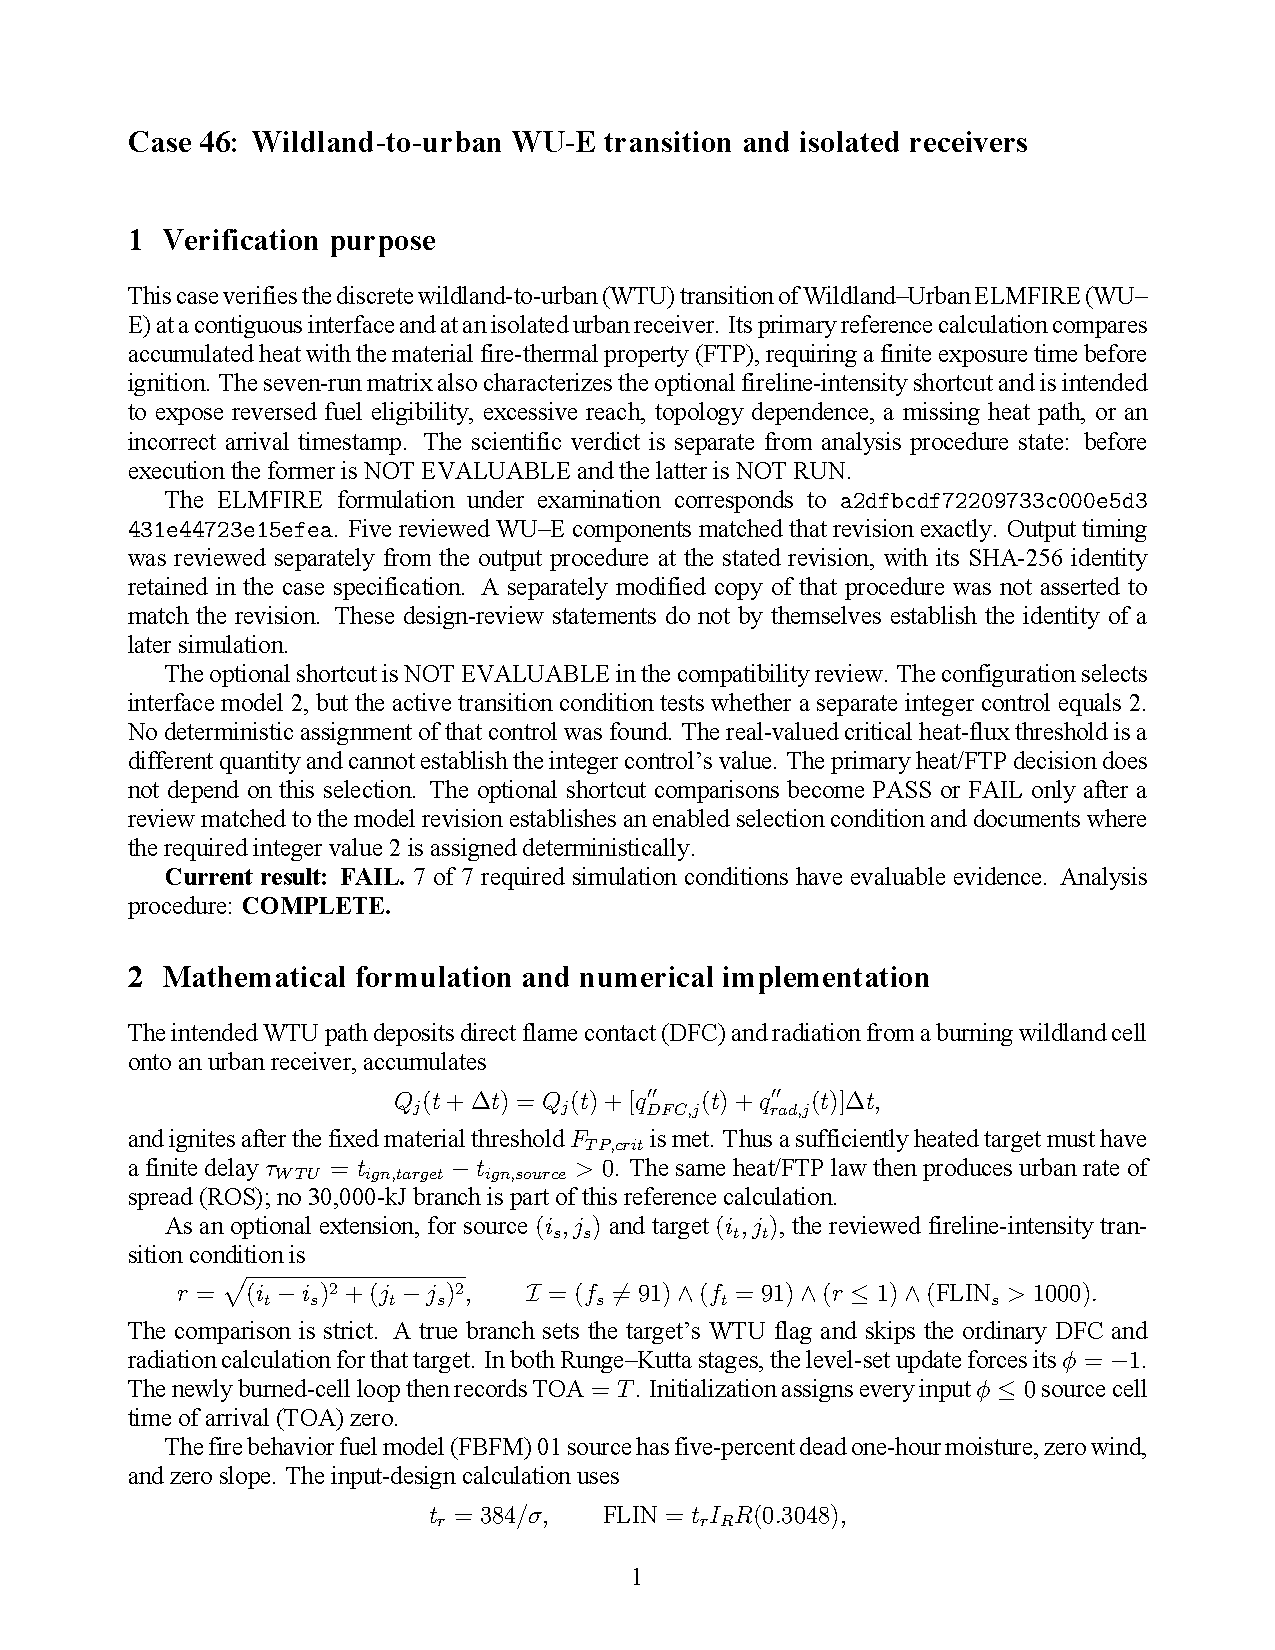
\includepdf[pages=-,pagecommand={\thispagestyle{empty}},addtotoc={1,section,1,{CASE46\_WUT -- Case 46: Wildland-to-urban WU-E transition and isolated receivers},case-detail:case46-wut}]{../cases/Verification/coupling_tests/CASE46_WUT/report/case_report.pdf}%
}{%
  \phantomsection
  \label{case-detail:case46-wut}
  \addcontentsline{toc}{section}{CASE46\_WUT -- Case 46: Wildland-to-urban WU-E transition and isolated receivers}
  \section*{CASE46\_WUT -- Case 46: Wildland-to-urban WU-E transition and isolated receivers}
  \textbf{NOT EVALUABLE:} the detailed case description is unavailable.
}

\clearpage
\IfFileExists{../cases/Verification/coupling_tests/CASE47_UWT/report/case_report.pdf}{%
  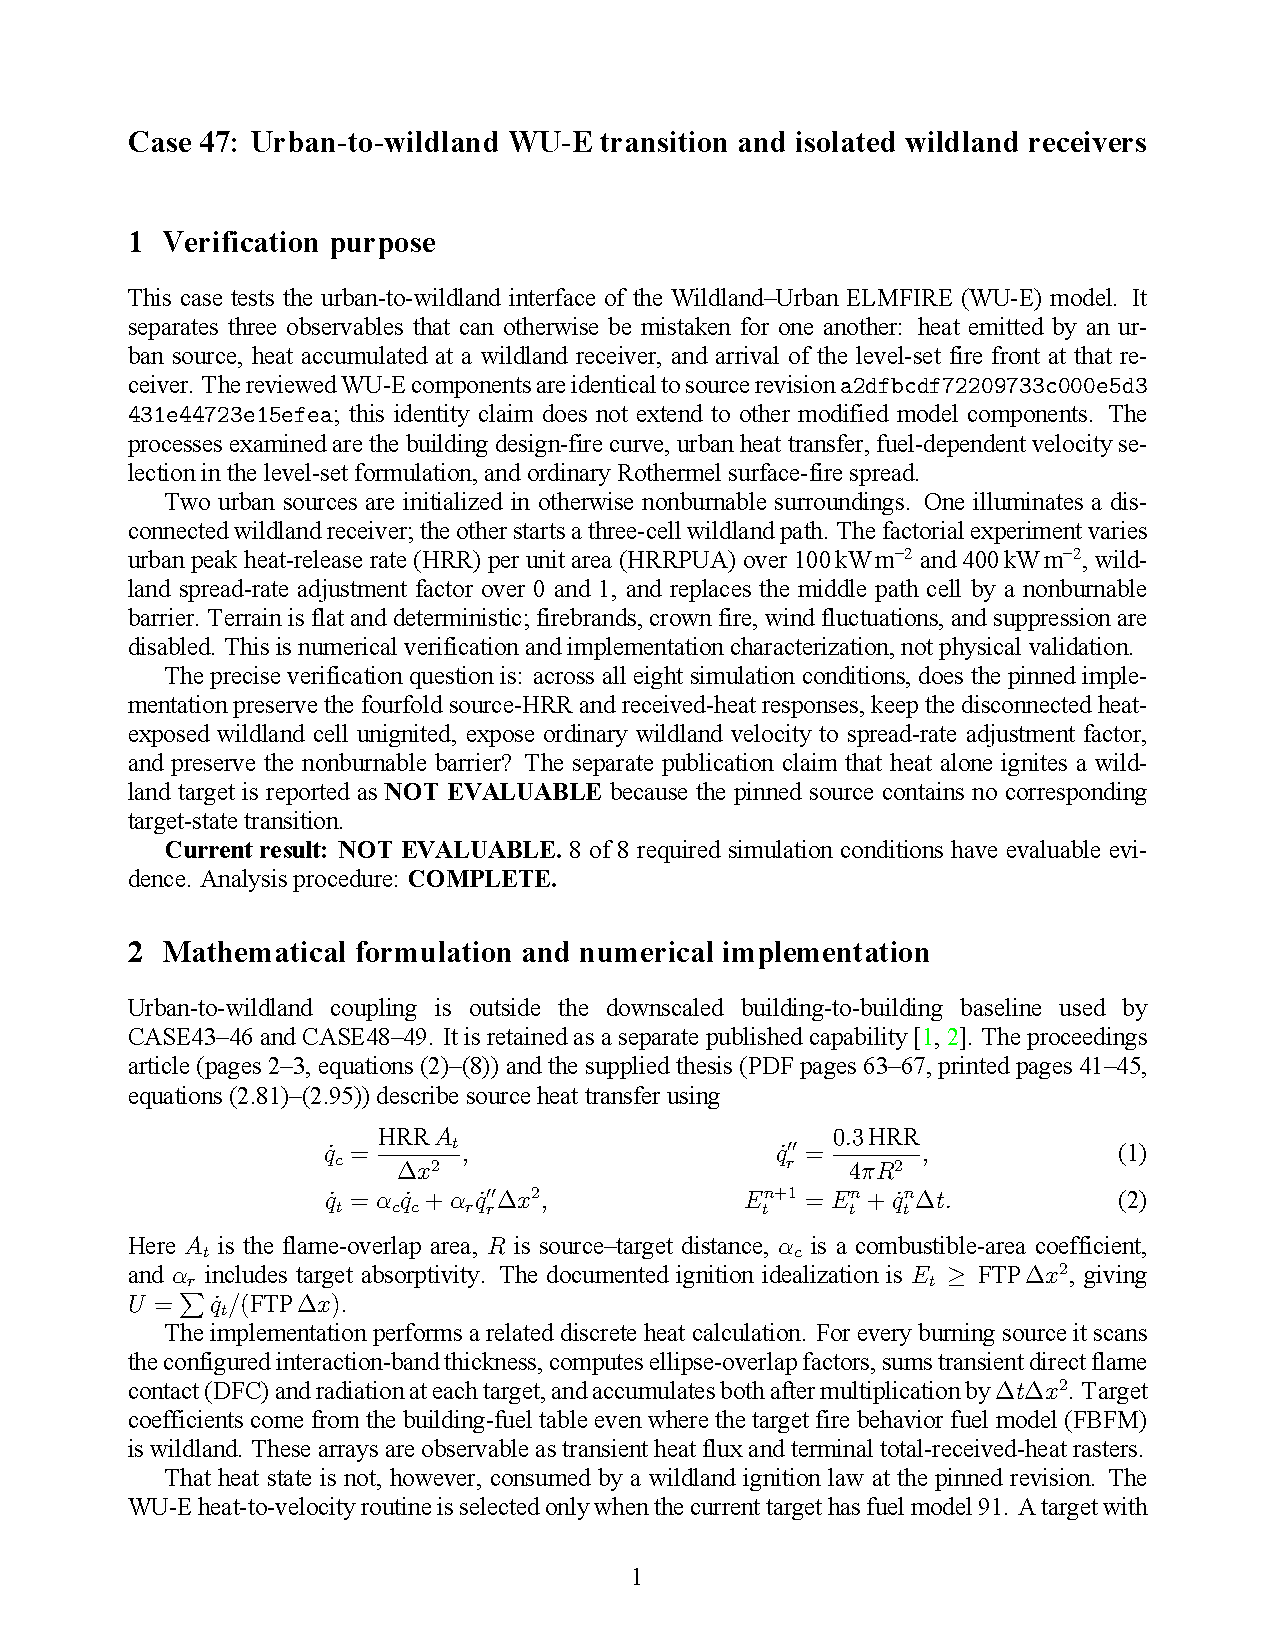
\includepdf[pages=-,pagecommand={\thispagestyle{empty}},addtotoc={1,section,1,{CASE47\_UWT -- Case 47: Urban-to-wildland WU-E transition and isolated wildland receivers},case-detail:case47-uwt}]{../cases/Verification/coupling_tests/CASE47_UWT/report/case_report.pdf}%
}{%
  \phantomsection
  \label{case-detail:case47-uwt}
  \addcontentsline{toc}{section}{CASE47\_UWT -- Case 47: Urban-to-wildland WU-E transition and isolated wildland receivers}
  \section*{CASE47\_UWT -- Case 47: Urban-to-wildland WU-E transition and isolated wildland receivers}
  \textbf{NOT EVALUABLE:} the detailed case description is unavailable.
}

\clearpage
\IfFileExists{../cases/Verification/coupling_tests/CASE48_WGC/report/case_report.pdf}{%
  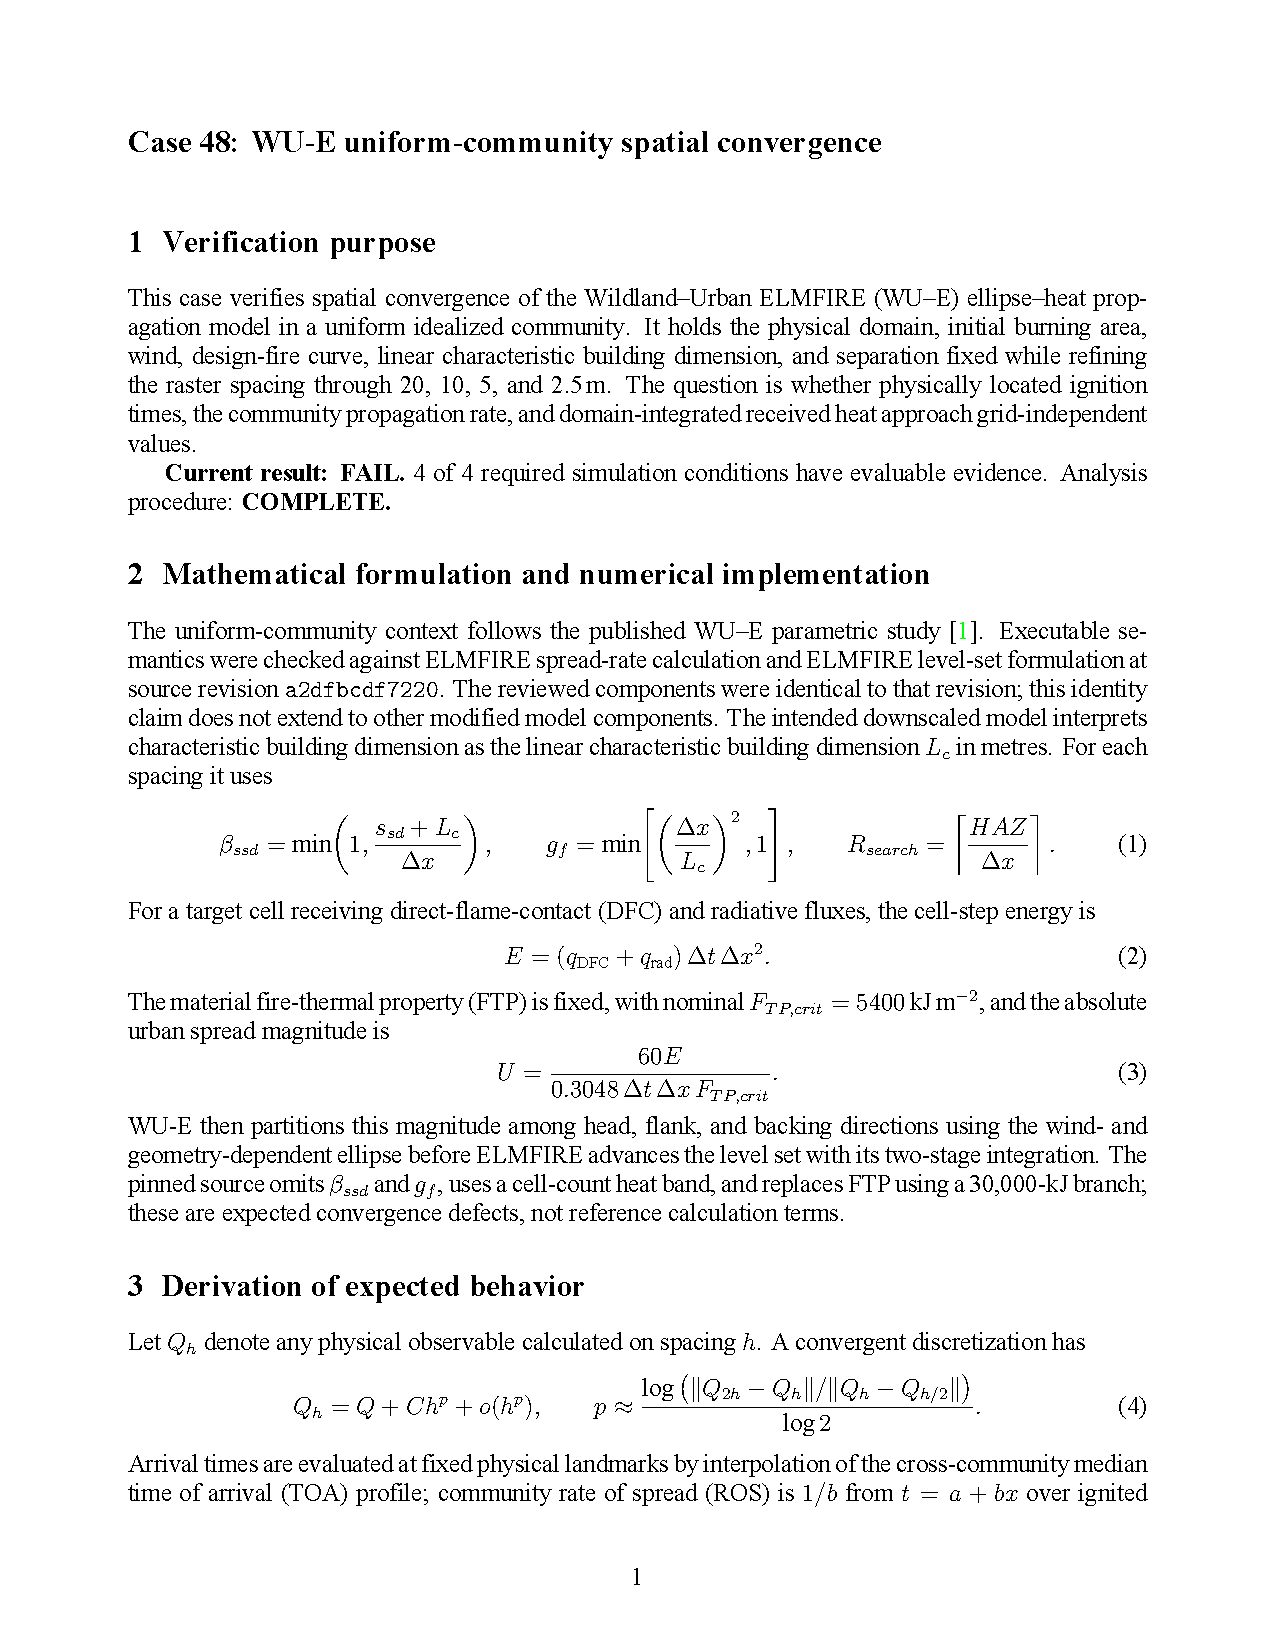
\includepdf[pages=-,pagecommand={\thispagestyle{empty}},addtotoc={1,section,1,{CASE48\_WGC -- Case 48: WU-E uniform-community spatial convergence},case-detail:case48-wgc}]{../cases/Verification/coupling_tests/CASE48_WGC/report/case_report.pdf}%
}{%
  \phantomsection
  \label{case-detail:case48-wgc}
  \addcontentsline{toc}{section}{CASE48\_WGC -- Case 48: WU-E uniform-community spatial convergence}
  \section*{CASE48\_WGC -- Case 48: WU-E uniform-community spatial convergence}
  \textbf{NOT EVALUABLE:} the detailed case description is unavailable.
}

\clearpage
\IfFileExists{../cases/Verification/coupling_tests/CASE49_WTC/report/case_report.pdf}{%
  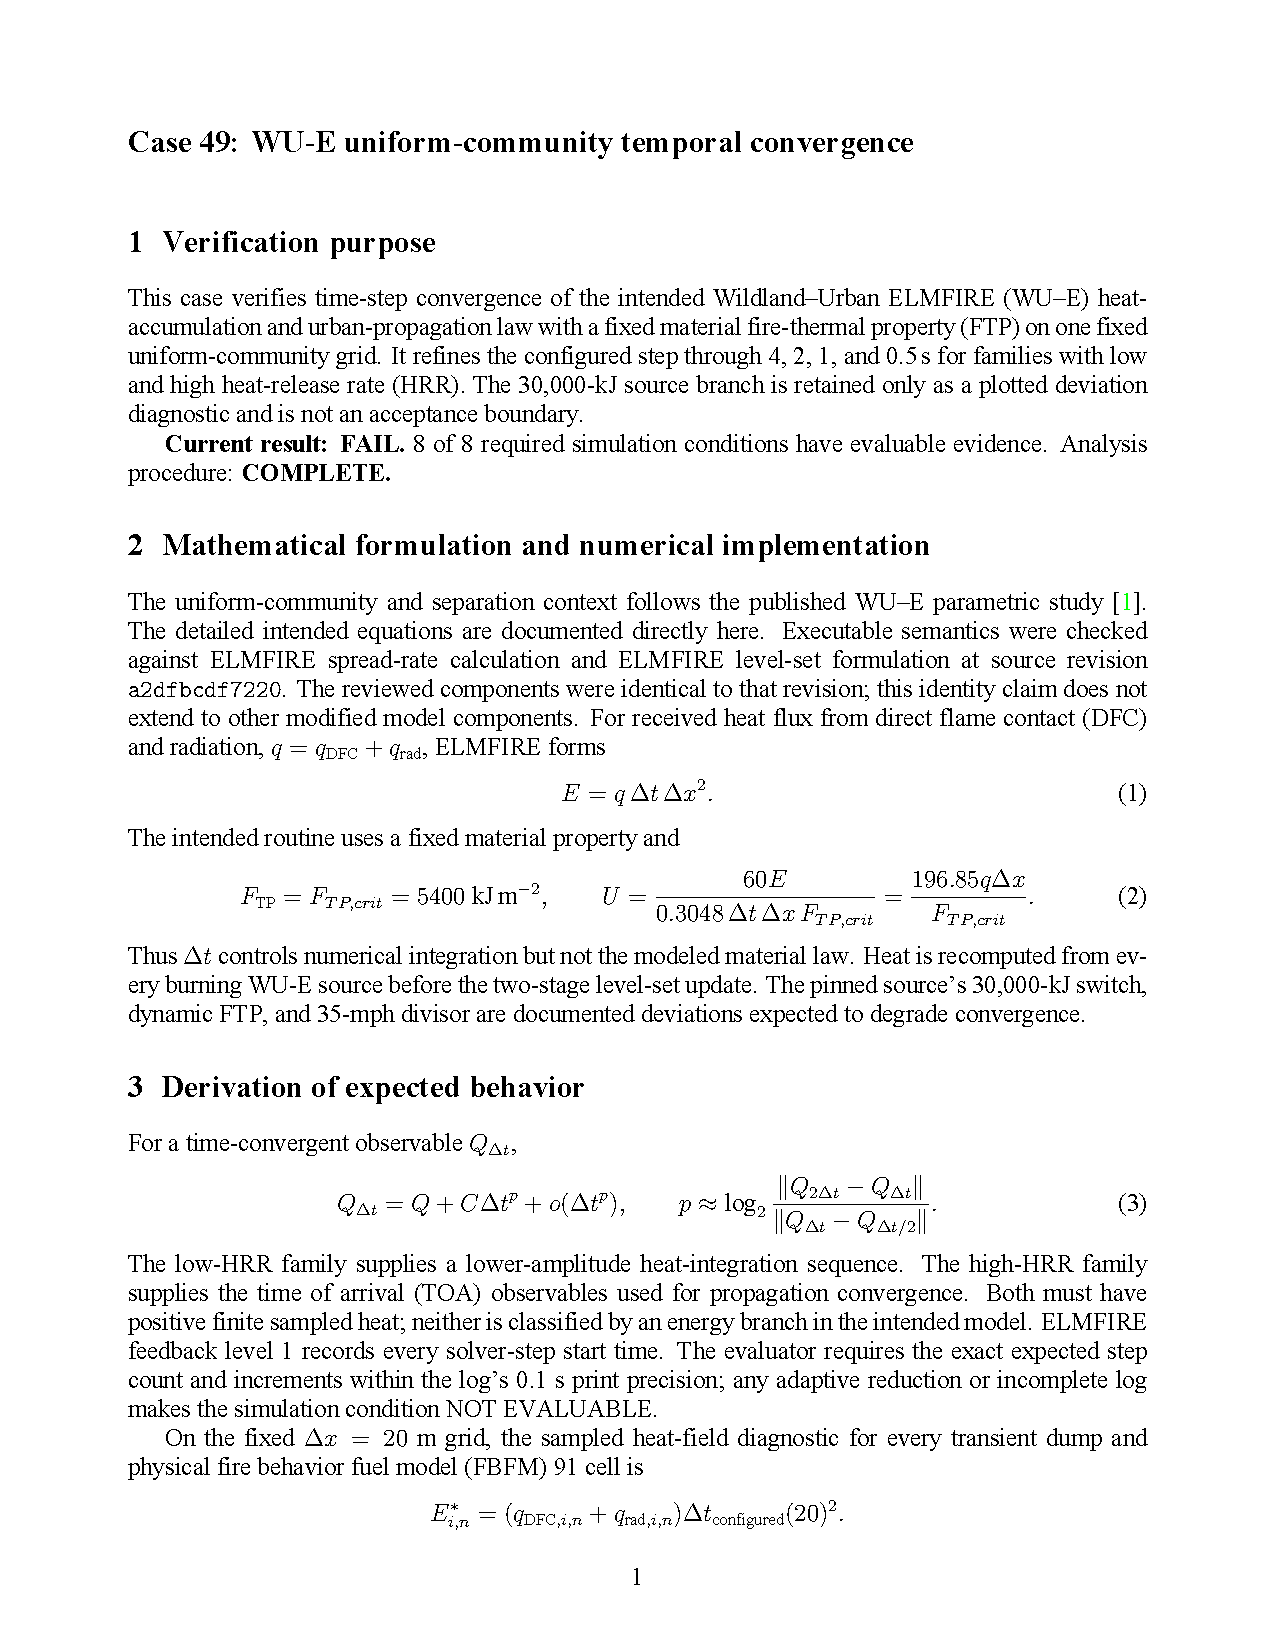
\includepdf[pages=-,pagecommand={\thispagestyle{empty}},addtotoc={1,section,1,{CASE49\_WTC -- Case 49: WU-E uniform-community temporal convergence},case-detail:case49-wtc}]{../cases/Verification/coupling_tests/CASE49_WTC/report/case_report.pdf}%
}{%
  \phantomsection
  \label{case-detail:case49-wtc}
  \addcontentsline{toc}{section}{CASE49\_WTC -- Case 49: WU-E uniform-community temporal convergence}
  \section*{CASE49\_WTC -- Case 49: WU-E uniform-community temporal convergence}
  \textbf{NOT EVALUABLE:} the detailed case description is unavailable.
}


\end{document}
